\documentclass[12pt,english,twoside]{article}
\usepackage[utf8]{inputenc}
\usepackage[a4paper]{geometry}
\geometry{verbose,tmargin=2cm,bmargin=2cm,lmargin=3cm,rmargin=2cm,headheight=12pt,headsep=24pt}
\setcounter{secnumdepth}{4}
\usepackage{titlesec}
\titleformat{\paragraph}
{\normalfont\normalsize\bfseries}{\theparagraph}{1em}{}
\titlespacing*{\paragraph}
{0pt}{3.25ex plus 1ex minus .2ex}{1.5ex plus .2ex}
\setcounter{tocdepth}{3}
\usepackage{pdfpages}
\usepackage{bm}
\usepackage{array}
\usepackage{float}
\usepackage{graphicx}
\usepackage{tocloft}
\usepackage{hyperref}
\hypersetup{
    colorlinks=true,
    linkcolor=blue,
    filecolor=blue,      
    urlcolor=blue,
}
\usepackage{setspace}
\PassOptionsToPackage{normalem}{ulem}
\usepackage{ulem}
\usepackage{indentfirst}	%Az összes címsor utáni bekezdést beljebb viszi%
\usepackage{amsmath}
\usepackage{tikz}
\usepackage{wrapfig}
\usetikzlibrary{shadings}
\usepackage{pgfplots}
\usepackage{hyperref}
\hypersetup{
    colorlinks,
    citecolor=black,
    filecolor=black,
    linkcolor=black,
    urlcolor=black
}

\usepackage{xcolor}
\usepackage{listings}

\definecolor{mGreen}{rgb}{0,0.6,0}
\definecolor{mGray}{rgb}{0.5,0.5,0.5}
\definecolor{mPurple}{rgb}{0.58,0,0.82}
\definecolor{backgroundColour}{rgb}{1,1,1}

\lstdefinestyle{CStyle}{
	backgroundcolor=\color{backgroundColour},   
	commentstyle=\color{mGreen},
	keywordstyle=\color{magenta},
	numberstyle=\tiny\color{mGray},
	stringstyle=\color{mPurple},
	basicstyle=\footnotesize,
	breakatwhitespace=false,         
	breaklines=true,                 
	captionpos=b,                    
	keepspaces=true,                 
	numbers=left,                    
	numbersep=5pt,                  
	showspaces=false,                
	showstringspaces=false,
	showtabs=false,                  
	tabsize=2,
	language=C
}


\makeatletter

%%%%%%%%%%%%%%%%%%%%%%%%%%%%%% LyX specific LaTeX commands.
\newcommand{\noun}[1]{\textsc{#1}}
%% Because html converters don't know tabularnewline
\providecommand{\tabularnewline}{\\}

%%%%%%%%%%%%%%%%%%%%%%%%%%%%%% Textclass specific LaTeX commands.
\newenvironment{lyxcode}
{\par\begin{list}{}{
\setlength{\rightmargin}{\leftmargin}
\setlength{\listparindent}{0pt}% needed for AMS classes
\raggedright
\setlength{\itemsep}{0pt}
\setlength{\parsep}{0pt}
\normalfont\ttfamily}%
 \item[]}
{\end{list}}

%%%%%%%%%%%%%%%%%%%%%%%%%%%%%% User specified LaTeX commands.
%\textwidth 160mm
%\oddsidemargin 0cm
%\topmargin -15mm
\usepackage{bm}
\newcommand{\tg}{\mathop\mathrm{tg}}
\newcommand{\grad}{\mathop\mathrm{grad}}
\newcommand{\BME}{\hrule\vspace{6pt}{\large Budapest University of Technology and Economics
\\
Faculty of Mechanical Engineering \\
Department of Applied Mechanics}}
\newcommand{\szerzo}{}
\newcommand{\konzulensek}{
\parbox[t]{20cm}
{\normalsize
\hspace*{25em} Made by:\\
\hspace*{28em}Bálint CSATÓ\\
\hspace*{25em}Supervisor:\\
\hspace*{28em}Gergely GYEBRÓSZKI \\
}\hfill}

\makeatother

\usepackage{babel}


\begin{document}



\title{\vspace{-2cm}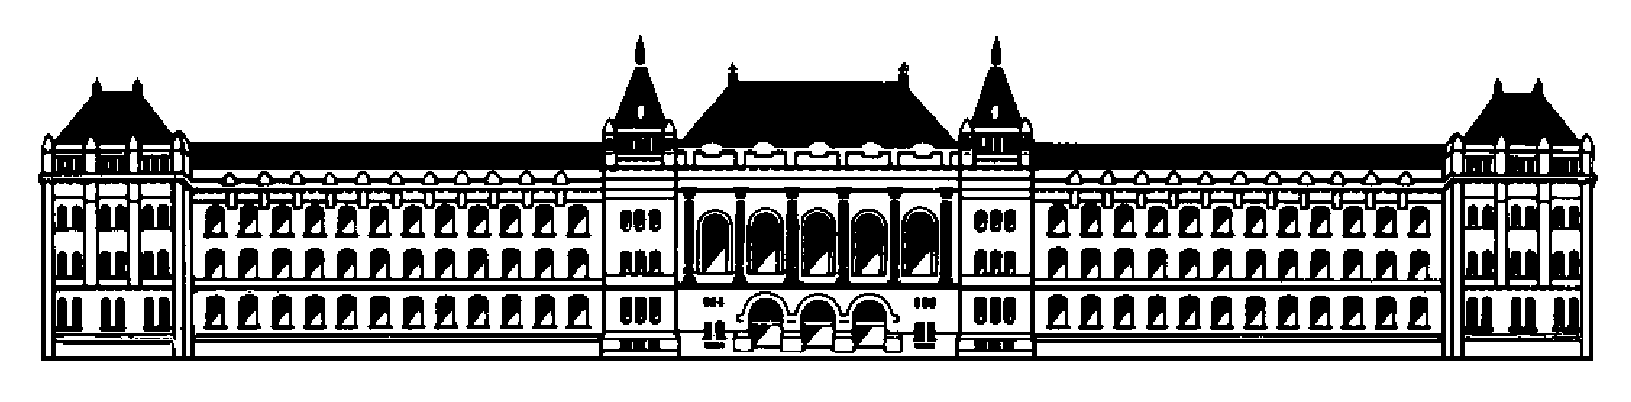
\includegraphics[width=0.4\textwidth,keepaspectratio]{figures/bme_skyline}\\
\BME\vspace{4cm}\\
Control and Parameter Estimation Problems of Autonomous Transport Robots
\\[5mm]
\large{Final Project}}


\author{\sc\szerzo}


\date{\vspace{6cm}\konzulensek\\
\vspace{3cm}Budapest, 2018}

\maketitle
\thispagestyle{empty}



\newpage
\pagenumbering{arabic}
\renewcommand{\contentsname}{Contents}
\renewcommand{\cftsecleader}{\cftdotfill{\cftdotsep}}
\tableofcontents
\numberwithin{equation}{section} % Number equations within sections
\numberwithin{figure}{section} % Number figures within sections
\numberwithin{table}{section} % Number tables within sections

\newpage

\section*{Abstract}
In this Final Project work the control and parameter estimation problems of an autonomous transport robot were investigated. A three-wheeled omnidirectional robot platform was built from scratch combined with the widely spread Arduino platform. In order to have a robot that behaves just as the user want, a detailed dynamic analysis and classical control of motors were carried out with great improvements in terms of location and orientation control. Additionally, the possibility of developing an on the go fall over avoidance autonomous feature was investigated for which a coupled electro-mechanical model was elaborated considering several details of the given hardware application. The developed fall over estimator model was compared with measurements and good agreements were obtained.

\addcontentsline{toc}{section}{Abstract}

\newpage

%%%%%%%%%%%%%%%%%%%%%%%%%%%%%%%%%%%%%%%%%%%%%%%%%%%%%%%%%%%%%%%%%%%%%%%%%%%%%%%%%%%%%%%%%%%%%%%%%%%%%%%%%%%%
% 													Preface
%%%%%%%%%%%%%%%%%%%%%%%%%%%%%%%%%%%%%%%%%%%%%%%%%%%%%%%%%%%%%%%%%%%%%%%%%%%%%%%%%%%%%%%%%%%%%%%%%%%%%%%%%%%%
\section*{Preface}
\addcontentsline{toc}{section}{Preface}
The basic motivations and the preliminary concept of this final thesis work was highly influenced by one of my former projects named Engineering problems of Autonomous Robots. Mainly the investigation of the environmental mapping functionality and requirements of an autonomous robot were analyzed with other colleges as a part of the subject called Teamwork Project at the Department of Applied Mechanics. During the semester, a simulator environment was built in which a robot, obstacles, bounds and moving algorithms could be defined. One can has a little glimpse to this concept with help of Figure \ref{glimpse}.
\begin{figure}[h]
	\centering
	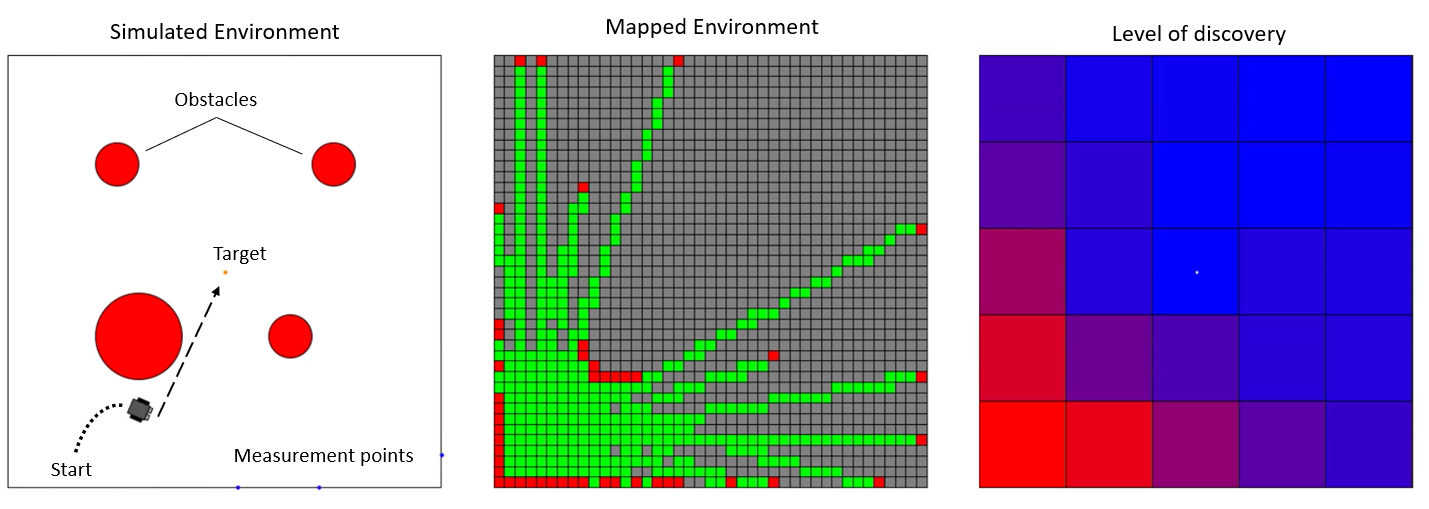
\includegraphics[width=\textwidth]{figures/glimpse.png}
	\caption{Environmental mapping algorithm}
	\label{glimpse}
\end{figure}

The main experiences were that for a successful environmental mapping algorithm the followings are essential:
\begin{itemize}
	\item Position and orientation estimation in the global frame
	\item Continuous distance measurement of the surrounding material points
	\item Obstacle avoidance and route planning
\end{itemize}

In the idealized simulator, the position and orientation estimation was the simplest task as it was nothing more just the integration of the hard coded velocities. The main purpose of the simulator was to develop the processing concept of the measurement of the material points around the robot an based on that data plan the next target where the robot should go optimally in order to discover the most unknown regions considering the surrounding obstacles that are needed to be avoided during the operation. Several searching algorithms such as Greedy or A* were tested with success for the given environment. 

In this project, beside the theoretical approaches also the possible hardware application was in focus. In parallel, a simple differential drive mobile robot was used and rebuilt to make it suitable for this purpose. The most of the issues were regarding the most fundamental, the so called low-level engineering problems such as make the robot go along a straight line and so on. Unfortunately, the robot's wheels did not have encoders equipped, thus only a rough odometry could be developed after circumstantial calibrations for a given surface. Additionally, only a simple one-dimensional ultrasonic sensor was attached which could be rotated using a servo motor. After the first measurements, it was clearly visible that higher focus must be concentrated on the accuracy of lower level features in order to have a sufficient chance to implement such an artificial intelligence operation in practice. Figure \ref{glimpse2} shows one of results of the environmental mapping measurement. In this case, the robot moved randomly driven by the obstacle avoidance algorithm and at several positions (red dots) made five-point distance measurement of material points (black dots) with ultrasonic sensor attached to a servo motor. It can be seen that the measurement points had a too high deviation to use in mapping processing. One of the main reason of the lack of accuracy was the inaccurate odometry.
\begin{figure}[h]
	\centering
	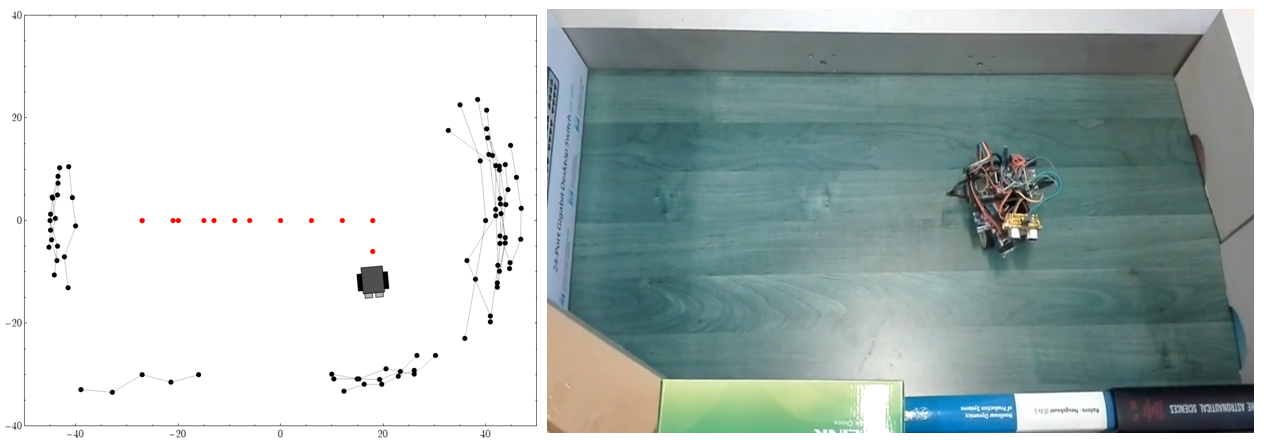
\includegraphics[width=\textwidth]{figures/glimpse2.png}
	\caption{Environmental mapping application on the robot platform}
	\label{glimpse2}
\end{figure}

As a conclusion, the main message of my former project was that one needs to go lower level first even if the final purpose is some kind of higher level autonomous operation. In case of this current transport robot project, these aspects were highly considered throughout out the selection and building of robot platform.


\newpage

%%%%%%%%%%%%%%%%%%%%%%%%%%%%%%%%%%%%%%%%%%%%%%%%%%%%%%%%%%%%%%%%%%%%%%%%%%%%%%%%%%%%%%%%%%%%%%%%%%%%%%%%%%%%
% 											Introduction to Autonomous Transport Robots
%%%%%%%%%%%%%%%%%%%%%%%%%%%%%%%%%%%%%%%%%%%%%%%%%%%%%%%%%%%%%%%%%%%%%%%%%%%%%%%%%%%%%%%%%%%%%%%%%%%%%%%%%%%%
\section{Introduction to Autonomous Transport Robots}
\subsection{History of transportation}

Since the early days of human civilization, one of the most common problem has been the transportation. The first major development was the domestication of animals that made it possible to transport more and heavier loads or humans themselves in order to achieve greater speed and duration capability. The next substantial invention was the wheel which increased the efficiency of animal based transportation introducing the concept of vehicles. Until the Industrial Revolution, the water transport facilities proved to be the most effective way. With the development of the combustion engines and automobiles around the end of the $19^{st}$ century, road transport became competitive again. Nowadays trucks move remarkable amount of cargo over thousands of miles, but light items in the environments near humans are still being carried in wheelbarrows or trailers attached to more compact vehicles. 

\begin{figure}[h]
	\centering
	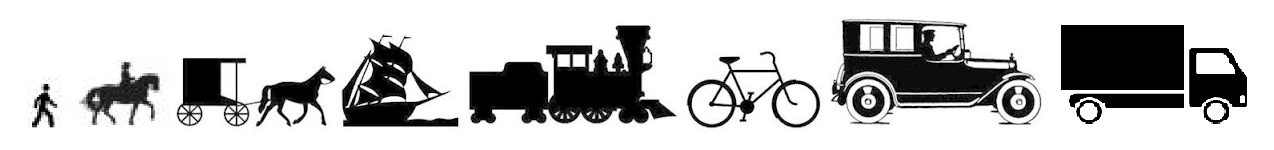
\includegraphics[height=1.5cm]{figures/evot.png}
	\caption{Evolution of Transportation \cite{google1}}
\end{figure}

\noindent One of the most dominant development tendency in almost every field of the industry is the automation of processes and procedures. Automation means the reduction of human intervention in the operation of machines. The prior benefit of automation is saving cost in terms of labor hours, therefore savings in costs regarding consumption such as electricity or some kind of material. Additionally, it helps to improve the quality and accuracy of processes by increasing the overall precision and making methods repeatable. The most trending application of the automation regarding transportation is the autonomous cars on the roads.
\subsection{Autonomous vehicles}
An autonomous car which is also known as a self-driving car or a driverless car is a vehicle that can operate without a certain amount of human control using its sensors to monitor the information coming from the environment. Great variety of techniques are used to detect the surroundings, such as radar, laser light, GPS, odometry and computer vision. The collected information provides a decent input to the control system which is the soul of the self-driving cars. Several control problems have to be solved continuously during driving on the roads, such as identifying obstacles and avoiding them, following transportation rules or navigating along a predefined path. 

Autonomous vehicle technology offers the possibility of fundamentally
changing transportation. Equipping cars and light vehicles
with this technology will likely reduce traffic collisions, thus the resulting injuries and the related costs including less need for insurance. Autonomous cars are predicted to increase the traffic flow and the mobility of citizens. Reduced traffic congestion and the improvements in traffic flow due to the widespread use of autonomous cars will also result in better fuel efficiency and reduced pollution in cities.

In spite of the various benefits also several issues exist such as technology challenges, disputes concerning liability, customer concerns about the safety of driverless cars, risk of loss of privacy and security concerns against hackers, risk of negative effects on the society and economy and finally moral issues when car's software is forced to choose between multiple undesired, e.g. harmful, alternatives during an inevitable accident. \cite{wiki}
 

The autonomous driving technology can be most easily conceptualized using a five-part
continuum suggested by the National Highway Traffic Safety Administration
(NHTSA), with different benefits of the technology realized
at different levels of automation: \cite{c}
\begin{itemize}
	\item \textbf{Level 0:}  The human driver is in complete control of all functions of the car.
	\item \textbf{Level 1:}  One function is automated.
	\item \textbf{Level 2:}  More than one function is automated at the same time (e.g., steering and acceleration), but the driver must remain constantly attentive.
	\item \textbf{Level 3:} The driving functions are sufficiently automated that the driver can safely engage in other activities.
	\item \textbf{Level 4:} The car can drive itself without a human driver.
\end{itemize}
\noindent

From an engineering point of view, the most important issues are the technological challenges, i.e. how to design a driverless vehicle which is at least as capable of handling vehicle's performance as a human in all possible conditions, or it may step beyond the edge of human capabilities. An autonomous vehicle is a combination of sensors and actuators, sophisticated algorithms executed as a software on a processor.

The sensory system can be classified into three different classes according to an article of Industrial Internet of Things (IIoT) World: \cite{5c}
\begin{itemize}
	\item \textbf{Navigation and guidance:} Basically, the system that deals with the localization and the control of movements of vehicles from a global point of view. In order to determine the location, the target place and the corresponding track between the two different techniques are used. The most common and well-know applications are the GPS, compass and dead reckoning.
	\item \textbf{Driving and Safety:} Directing the vehicle and making sure that vehicle follows the rules of the road. The autonomous car must be able to see and interpret what is in front of it when it is going forward (and behind in reversing case). It is also necessary to see what is on either side, in other words, it needs a 360$^{\circ}$ view. A set of video cameras is an obvious choice by which location of lanes and surrounding objects or markers on the road can determined.
	\item \textbf{Performance:} The most indispensable function is the management of the internal system of the car. Even the human driven vehicles have to be equipped by several specific sensors by means of feedbacks can be provided of essential parameters such as the speedometer or fuel load monitor. In case of an autonomous vehicle that tends to operate in a more sophisticated way, several unique electronic circuits and special sensors have to be added compared to a conventional vehicle to provide the functions needed for autonomous driving. With the help of more complex sensory system, a more accurately and robustly optimized power control is possible during operation with ceratin conditions in terms of overall consumption, component amortization, thermal and noise dissipation.
\end{itemize}

The concept of driverless cars made a lot of attention over the past ten years. Generally speaking, it can be said that one of the most determining development directions in the automotive industry are related to automated solutions. Many people still do not believe that there could be such a possibility with fully driverless vehicles due to the fact that there so many parameters in the driving functions that have to be controlled simultaneously and continuously and even a single failure could cause serious catastrophe. Nowadays after a lot of research and experiments, self-driving cars can be seen as a reality, or at least something that can be a close future. Still, there are many challenges in designing a fully autonomous system for a self-driving car. The challenges of driverless cars can be sorted into five groups: \cite{5c}

\begin{itemize}
	\item  \textbf{Road conditions:} 
	Road conditions can be unpredictable and varying, i.e. in some cases they are smooth and well-marked while in other cases there are no lane marking. On some roads there can be potholes, in case of mountainous and tunnel roads the visibility of external signals for direction are poor.
	
	\item 	\textbf{Weather conditions:}
	It can be sunny and clear or rainy and stormy weather. Autonomous cars have to work in all weather conditions, there is no scope for any failure.
	
	\item \textbf{Traffic conditions:}
	Maybe this is the most complex problem as the human behavior and autonomous car algorithm have to be matched with each other. The cars would have to drive in all sorts of traffic conditions as humans are capable of. The people are emotional beings operating irrationally sometimes which is basically hardly foreseeable. Besides the fact that the traffic would be highly self-regulated, in certain cases some people might break the rules resulting an unpredictable situation in point of a self-driving car. Additionally, also an object may turn up in an unexpected conditions, e.g. crashed car which have to be bypassed ignoring some traffic rules. It can be handled by humans easily but for an artificial intelligence it is a harder task as its operation is ruled by rule-following conditions and this kind of situation needs the capability of detecting the need to ignore the rules in that specific case. The lack of intelligence of several autonomous cars on the roads could result in traffic deadlock or even crashes.
	
	\item \textbf{Accident Liability:}
	One of the most important aspects of autonomous cars are accidents liability questions, thus the liable for the accident caused by a driverless car has to be determined.
	Typically, the software will be the main component that drives the car and makes all the good and bad decisions. At initial levels of design there is a person who is physically behind the steering wheel and can take over the control, but in newer designs does not have even any dashboard, pedals and steering wheel. In such cars, the driver who is actually almost just a passenger cannot be liable for an accident. Furthermore, due to the nature of autonomous cars, the drivers can be supposed to be in a relaxed state without paying sufficient attention to handle unexpected traffic conditions, thus by the time the intervention action would be needed, it may be too late.
	
	\item \textbf{Radar Interference:}
	Autonomous cars use lasers and radar for navigation. The principle of work of radar is based on detecting reflections of radio waves from surrounding objects. The time taken for the reflection is measured to calculate the distance between the car and the object and appropriate action is then taken based on the radar readings. The problems will come up when thousands of cars on the roads try to use the technology because the reflected radar signals can interfere with each other making it difficult to distinguish which signal was emitted by which vehicle. Even if choosing a different radio frequency can eliminate the issue, the available frequency range is unlikely sufficient for all the vehicles manufactured.
	\cite{5c}
\end{itemize}
As a conclusion, it can be stated that there are still a lot of challenges besides the fact that there have been already some autonomous cars on the roads nowadays, but mostly for development and research purposes. Probably, the collective effort of the industry will definitely make the autonomous car in everyday life a reality one day since the benefits are considered to be remarkable. The most important expected benefit would be the reduction of losses of life in road accidents. Benefits with secondary importance are the reduction of fuel consumption, therefore the environmental pollution caused by vehicles, furthermore time and cost savings could be realized due to optimized behavior, e.g. traffic congestion free cities. Time, cost and energy savings are top wanted purposes in almost every field of industry and everyday life, therefore autonomous solutions with such desired features will likely appear in more and more applications. 

\subsection{Application of autonomous transport robots}
The conventional ways of transporting could be appropriate for most of the cases but not in those when repeated passages to specific locations in small distances have to be taken.
One of the latest trends in technology is to create such driverless robots that can help people in their everyday life, i.e. bringing any kind of products to customers. A company called Starship launched a several self-driving robotic vehicles on the streets of Washington, D.C. that can transport food and other small items to customers ordering via app.

\begin{figure}[htb!]
	\minipage{0.48\textwidth}
	\centering
	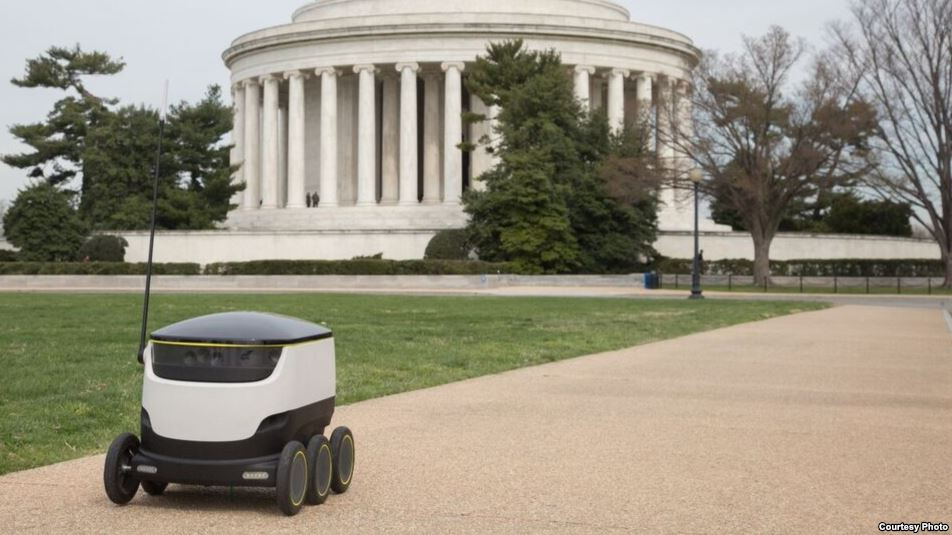
\includegraphics[height=4cm]{figures/starship.jpg}
	\label{fig1}
	\caption{Starship Technologies: Food ans small item transport robot \cite{starship}}
	\endminipage\hfill
	\minipage{0.48\textwidth}
	\centering
	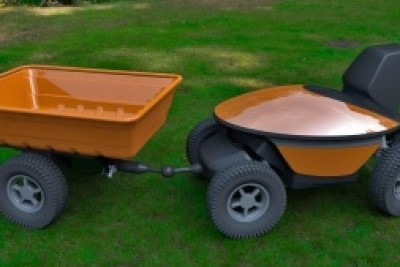
\includegraphics[height=4cm]{figures/smp.jpg}
	\label{smp}
	\caption{SMP Robotics: Garden garbage collector and transport robot \cite{smp}}
	\endminipage\hfill
\end{figure} 
The robotic vehicles move themselves along sidewalks using camera and tracking technology to avoid any obstacle and its location can be tracked from the distance in order to know the time of arrival. The six-wheeled electric machine sits about a half-meter high having a lockable cargo bay to carry food products up to nine kilograms in weight.\cite{starship}

A company called SMP Robotics made automated guided vehicles that can remove grass clippings and fallen leaves or construct garbage collection in a garden. These small-sized mobile robots have a trailer attached to the back. They are powered by electrical engines, thus noise and smell emission is minimized what allows operation around people. The built-in accumulators stores the needed energy and can last for several days of cyclical operation. Two ways of route following methods are available. The first option is to choose a root in advance with the help of the attached PC tablet. The second way is to set the robot in its 'follow me' algorithm whereby it is going to follow the operator and learn the path. The collected goods on the trailer can be unloaded automatically using a mechanism without any human intervention. The trailer can be fitted with a water tank which can be used for watering of grass and other plants, furthermore automatic water refill algorithm is implemented. This kind of automatic self-moving watering system suits really well such occasions when a fixed irrigation systems are not worth being built due to climate characteristics.\cite{smp}

A firm named NEOBOTIX made autonomous transport systems for daily use in industrial applications. The robots are equipped with laser scanners that permanently detect landmarks and obstacles which allows the robot to react dynamically to unexpected changes of their surrounding, i.e. to safely operate between human and other moving objects. This flexibility makes them suited for dynamic transportation tasks with frequent changes. For instance, they can complement roller or belt conveyors and take parts to machines or workplaces that are not connected to the conveyor system. \cite{neo}

\begin{figure}[htb!]
	\centering
	\minipage{0.48\textwidth}
	\centering
	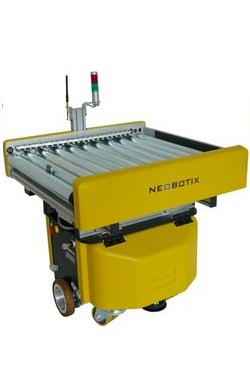
\includegraphics[height=5cm]{figures/neo1.jpg}
	\caption{{\small NEOBOTIX MT-400 Industrial Transport Robot \cite{neo}}}
	\endminipage\hfill
	\minipage{0.48\textwidth}
	\centering
	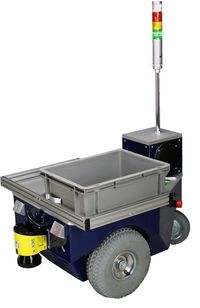
\includegraphics[height=5cm]{figures/neo2.jpg}
	\caption{{\small NEOBOTIX MT-500 Industrial Transport Robot \cite{neo}}}
	\label{conv2}
	\endminipage\hfill
\end{figure} 

\noindent Possible applications are taking parts to and from workplaces, transporting in direct interaction with humans or dynamic picking of parts for later assembly

BMW logistics also uses autonomous transport robots similarly in industrial environment. The well-known car manufacturer has been working hard to reduce emissions in all steps of the manufacturing process of a car, not only in the final product. This application shows really well that the autonomous developments in the automotive industry is not just about the autonomous driving on the roads but the manufacturing processes as well. Smart Transport Robots (STR) transport components through logistics at the Wackersdorf plant. They measures the distance to wireless transmitters which are located at in the logistics hall to calculate its exact position and route. The robot is capable of sharing the route with humans and other vehicles with the help of its sensors by identifying and reacting to critical situations. \cite{bmw}

\begin{figure}[htb!]
	\centering
	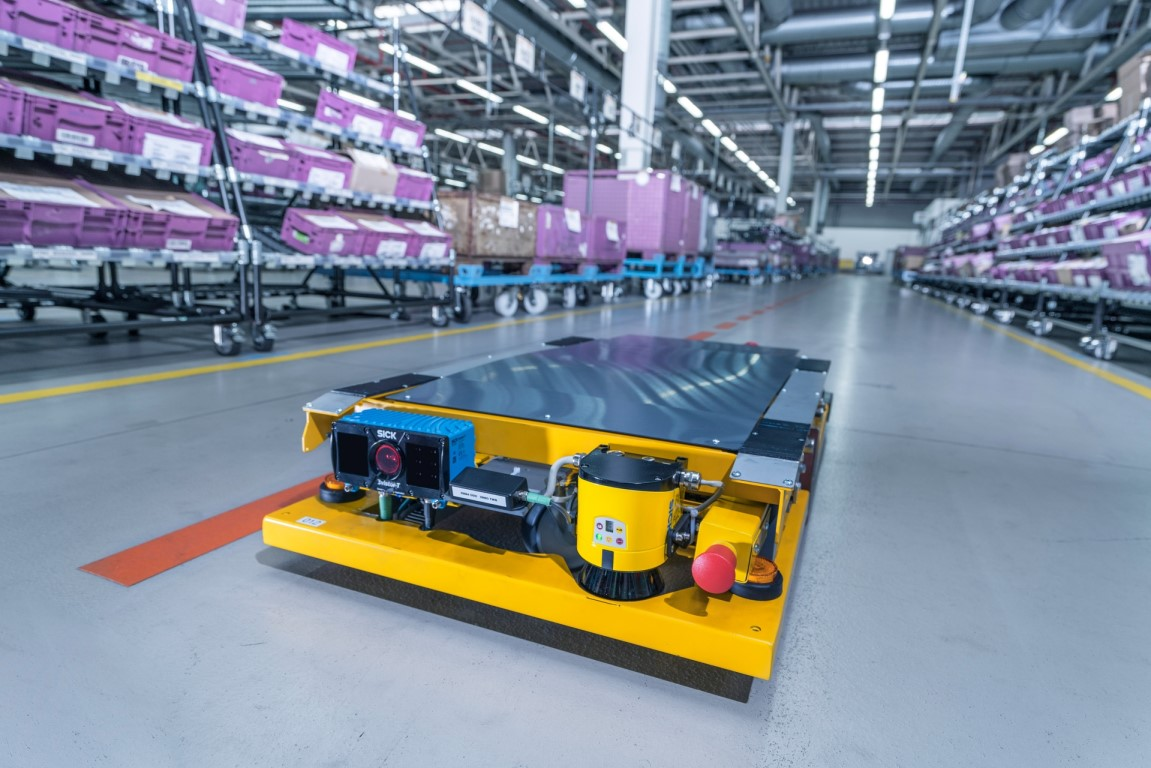
\includegraphics[width=9cm]{figures/bmw.jpg}
	\label{bmw}
	\caption{BMW: Smart Industrial Transport Robots  \cite{bmw}}
\end{figure}

A company, named AETHON, made fully autonomous robot called TUG that automates the transport of materials and supplies in commercial environments. It can automatically drop off and pickup of carts, navigates on internal map of facility using laser and it has a omnidirectional 4 wheel driven drive system for higher maneuverability.

\begin{figure}[htb!]
	\centering
	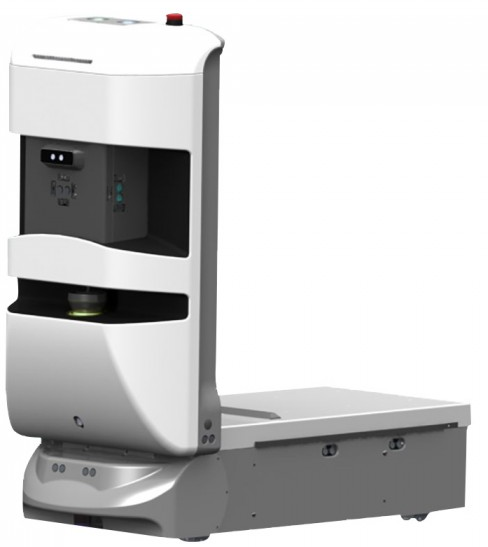
\includegraphics[width=7cm]{figures/tug.png}
	\label{bmw}
	\caption{AETHON: TUG mobile commercical transport robot of materials and supplies}
\end{figure}

Another interesting field of application of transportation robots is the military. Humans doing this kind of work are often exposed to a risk which would be great to avoid. The Autonomous Platform Demonstrator is a military transportation robot developed by the U.S. It has a hybrid-electric drive train with six in-hub electric motors powered by li-ion batteries charged using an on-board diesel generator. 

\begin{figure}[h]
	\centering
	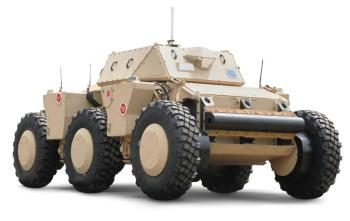
\includegraphics[width=7cm]{figures/apd.jpg}
	\label{bmw}
	\caption{Military transportation robot: APD}
\end{figure}

From control point of view it can be controlled in real-time by a soldier or it can operate autonomously. Autonomously it can operate at speeds up to 50 mph. Furthermore, it can travel along a GPS way point route and avoid obstacles in its way. \cite{apd}


\newpage

\section{Mobile Robotics}
The general platform of the transportation robots is obviously the family of mobile robots. Usually, a mobile robot faces more design challenges compared to robots that operates in fixed positions as it is left alone in the world. The most critical design problem is related to the locomotion which has to be suited with the conditions of the given ground. In order to handle the changes of the environment and to be able to make decisions during runtime as a function of actual state, the robots need to have more intelligence and self-determination. The mobile robots are still not reliable enough nowadays to operate in wide ranges outside of laboratory walls. They need to have a built-in model about their environment, furthermore they need to detect and analyze that of changes and their actual positions have to be found in order to be able to design and perform the next movements. In other words, a sequence of intelligent acts are expected to be carried out based on interactions with the dynamically changing outside world.
\subsection{Classification of mobile robots}
\subsubsection{Based on the medium in which the robot moves}
\begin{itemize}
	\item \textbf{Air/Space} \\
		These are mostly applied in space flight and military. The most well known application is the Unmanned Aerial Vehicle (UAV), commonly known as drone which is an aircraft without a pilot. The drones develop fast as they are easier to build and control as they do not have to navigate between obstacles.
	\item \textbf{Water} \\
		Automated Underwater Vehicles (AUV) are generally used in seas and oceans for research and industrial purposes. One of the most interesting field is the development of amphibious vehicle that can operate either on earth or on water.
	\item \textbf{Earth} \\
		As it is our natural habitat, the robots operating on earth are the most common.	\cite{sieg} \cite{rirt}
\end{itemize}
\subsubsection{Based on the locomotion mechanism}
Mobile robots generally locomote either using wheeled mechanism, a well-known human technology for vehicles, or using a small number of articulated legs being inspired by biological systems. Generally, legged locomotion demand more degrees of freedom and therefore greater mechanical complexity than wheeled locomotion. Wheels, in addition to being simple, are extremely well suited to flat and hard ground, thus their energy need is radically less compared to legged locomotion. However, the softer the surface, the higher the rolling friction which results a dramatic efficiency loss in case of wheeled robots. The efficiency of wheeled locomotion depends on the flatness and hardness of the ground, while the efficiency of legged locomotion depends on the leg mass and body mass. Nature prefers the legged locomotion since they must operate on rough and unstructured terrain where a wheeled vehicle could get stuck easily, e.g. in case of Sojourner Mars rover in 1997. They are simply unable to step over an obstacle, the only chance is to avoid it.
On the other hand, it is also understandable that the most of the industrial applications of mobile robotics utilize some form of wheeled locomotion due to the fact that the human environment mostly consists of smooth surfaces, both indoors and outdoors. In such conditions, the wheeled configurations are currently faster, less complex to design and more mobile.

In locomotion, the mobile robot moves in the fixed environment as a result of the propulseur forces. The scientific basis is the study of actuators that generate interaction forces and the mechanisms that implement the desired kinematic and dynamic requirements. The core issues that are needed to be evaluated to analyze a robot configuration in terms of locomotion are the followings: \cite{sieg}
\begin{itemize}
	\item Stability
		\begin{itemize}
			\item number and geometry of contact points
			\item center of gravity
			\item static/dynamic stability
			\item inclination of terrain
		\end{itemize}
	\item Characteristics of contact
		\begin{itemize}
			\item contact point/path size and shape
			\item angle of contact
			\item friction
		\end{itemize}
	\item Type of environment
	\begin{itemize}
		\item structure
		\item medium, (e.g. water, air, soft or hard ground)
	\end{itemize}

\end{itemize}


\subsection{Legged Mobile Robots}
Legged mobile robots contact the ground by a set of contact points which provides good adaptability and maneuverability in rough terrains. Not even the ground quality is an issue until the ground clearance is possible to be maintained, e.g crossing holes which does not exceed the size of the robot is a solvable demand. The main disadvantages of legged systems include power and mechanical complexity. The leg must be capable of sustaining the part of the robot’s total weight, lifting and lowering the robot body meanwhile keeping the stability permanently. Furthermore, high maneuverability needs sufficient number of degrees of freedom to impart forces in a sufficient number of different directions.
The legged robots are basically biologically inspired based on the fact that they are successful locomotion systems. A number of different leg configurations have been successful in a variety of organisms, i.e. the most common numbers are the two, four or six.

\begin{figure}[h]
	\centering
	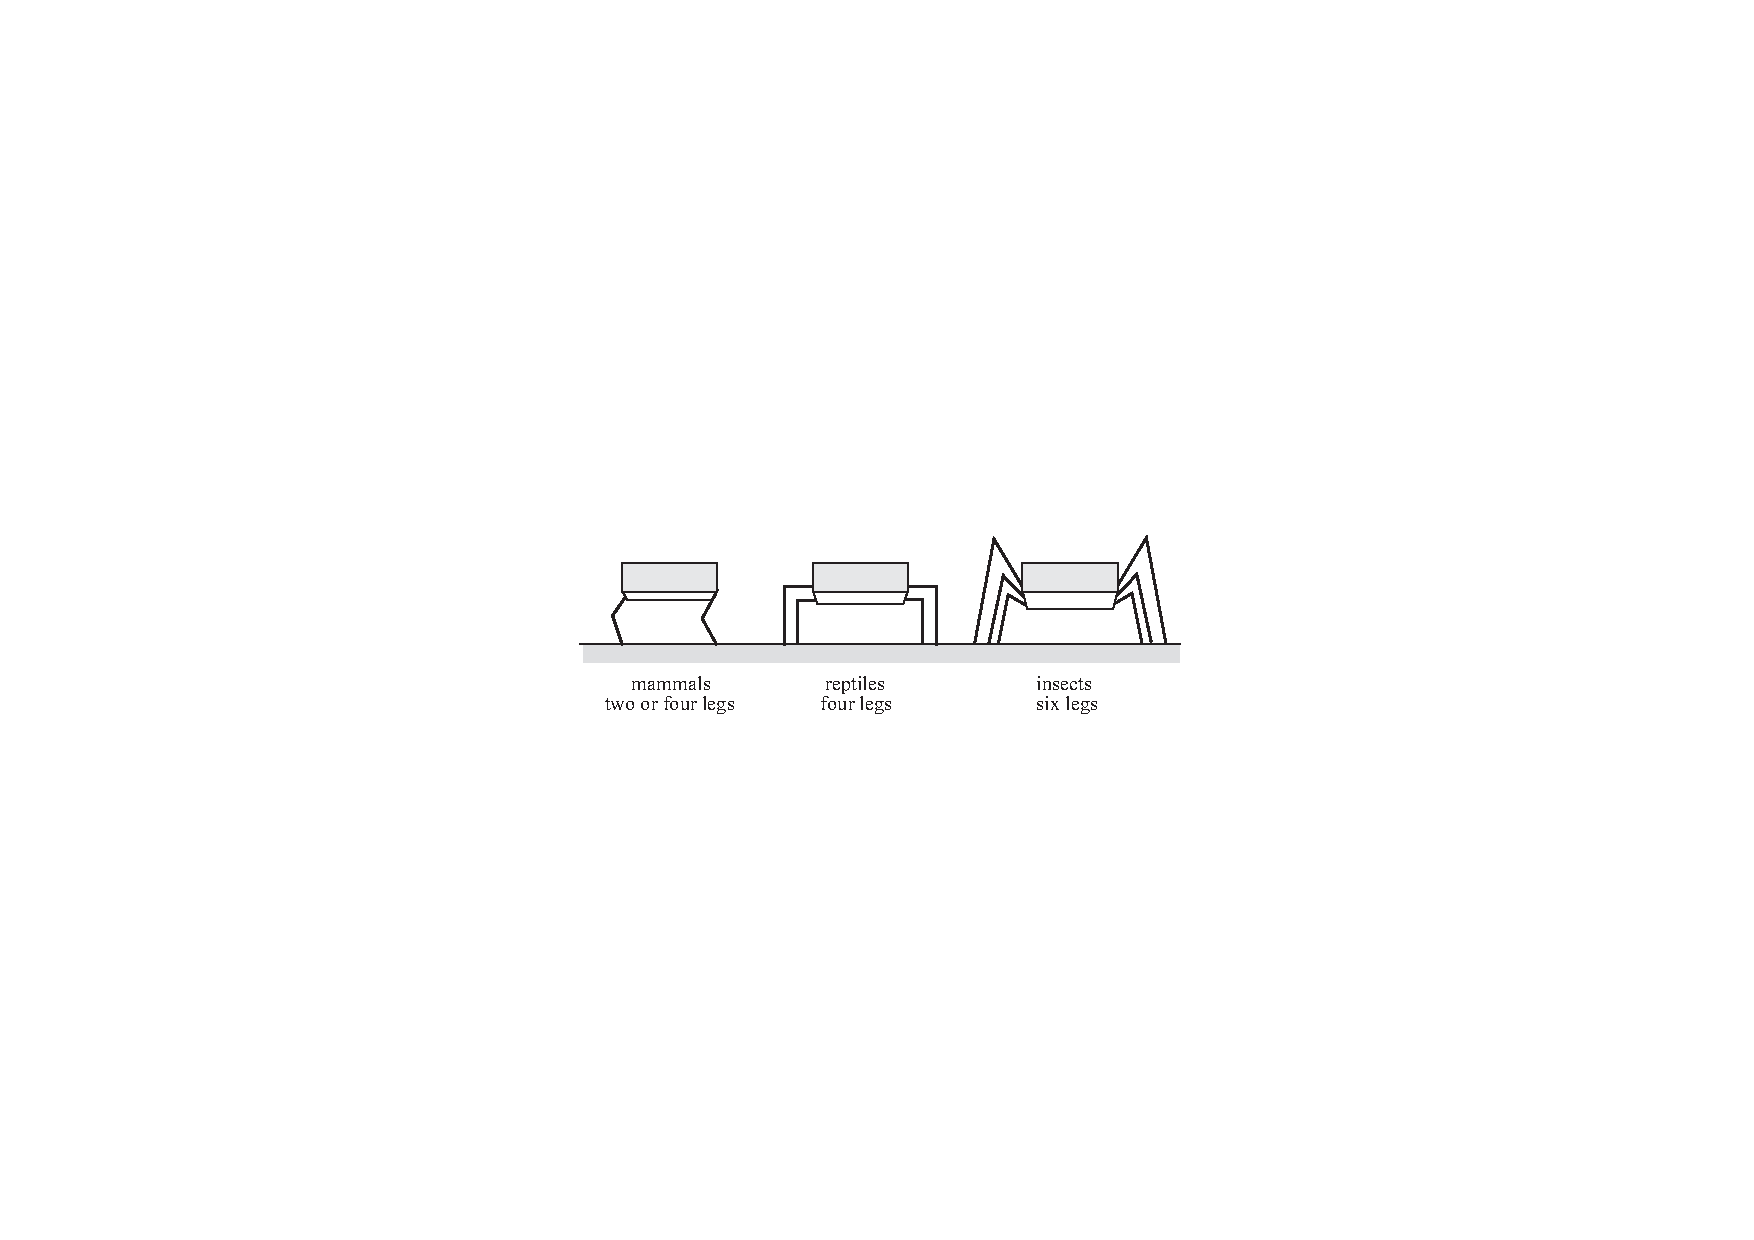
\includegraphics[width=7cm]{figures/legged2.pdf}
	\label{legged}
	\caption{Arrangement of the legs of various animals \cite{sieg}}
\end{figure}

A creature with at least three legs can achieve static balance which means that no correcting movements have to be taken to preserve its balance. Actually static balance means that the center of gravity is within the tripod of ground contact. A small perturbation in stability is passively corrected toward the stable pose by constrain forces after the disturbance goes away. However, any creature who is intended to walk must be able to lift and then release their legs, thus for static walking the minimum number of needed legs is six. Insects and spiders are immediately able to walk when born compared to mammals with four legs who are not able to walk or even to stand in case of humans with only two legs. Therefore the main issue regarding the locomotion of legged robots is the balancing. Of course, the number of legs and also the number of degrees of freedom of a given leg can be increased in order to achieve better stability and maneuverability. On the other hand, more legs and joints result more actuators, thus more energy, more mass, more control complexitiy, i.e. more costs in certain senses. Most of the legged robots in research and industrial cases have two legs.
The robot legs and arms are usually driven by electrical motors and pneumatic pistons. High level of harmony of the piston movements must be carried out by the designer in order to hold its balance also during the walking which is a challenging control task. \cite{sieg}

\subsection{Wheeled Mobile Robots}
The wheels are the most widely used locomotion mechanisms in man-made vehicles in general due to its simplicity, effectiveness. In most of the cases, during the design the robot builders need to focus problems regarding traction, stability, maneuverability and control. 

\begin{figure}[h]
	\centering
	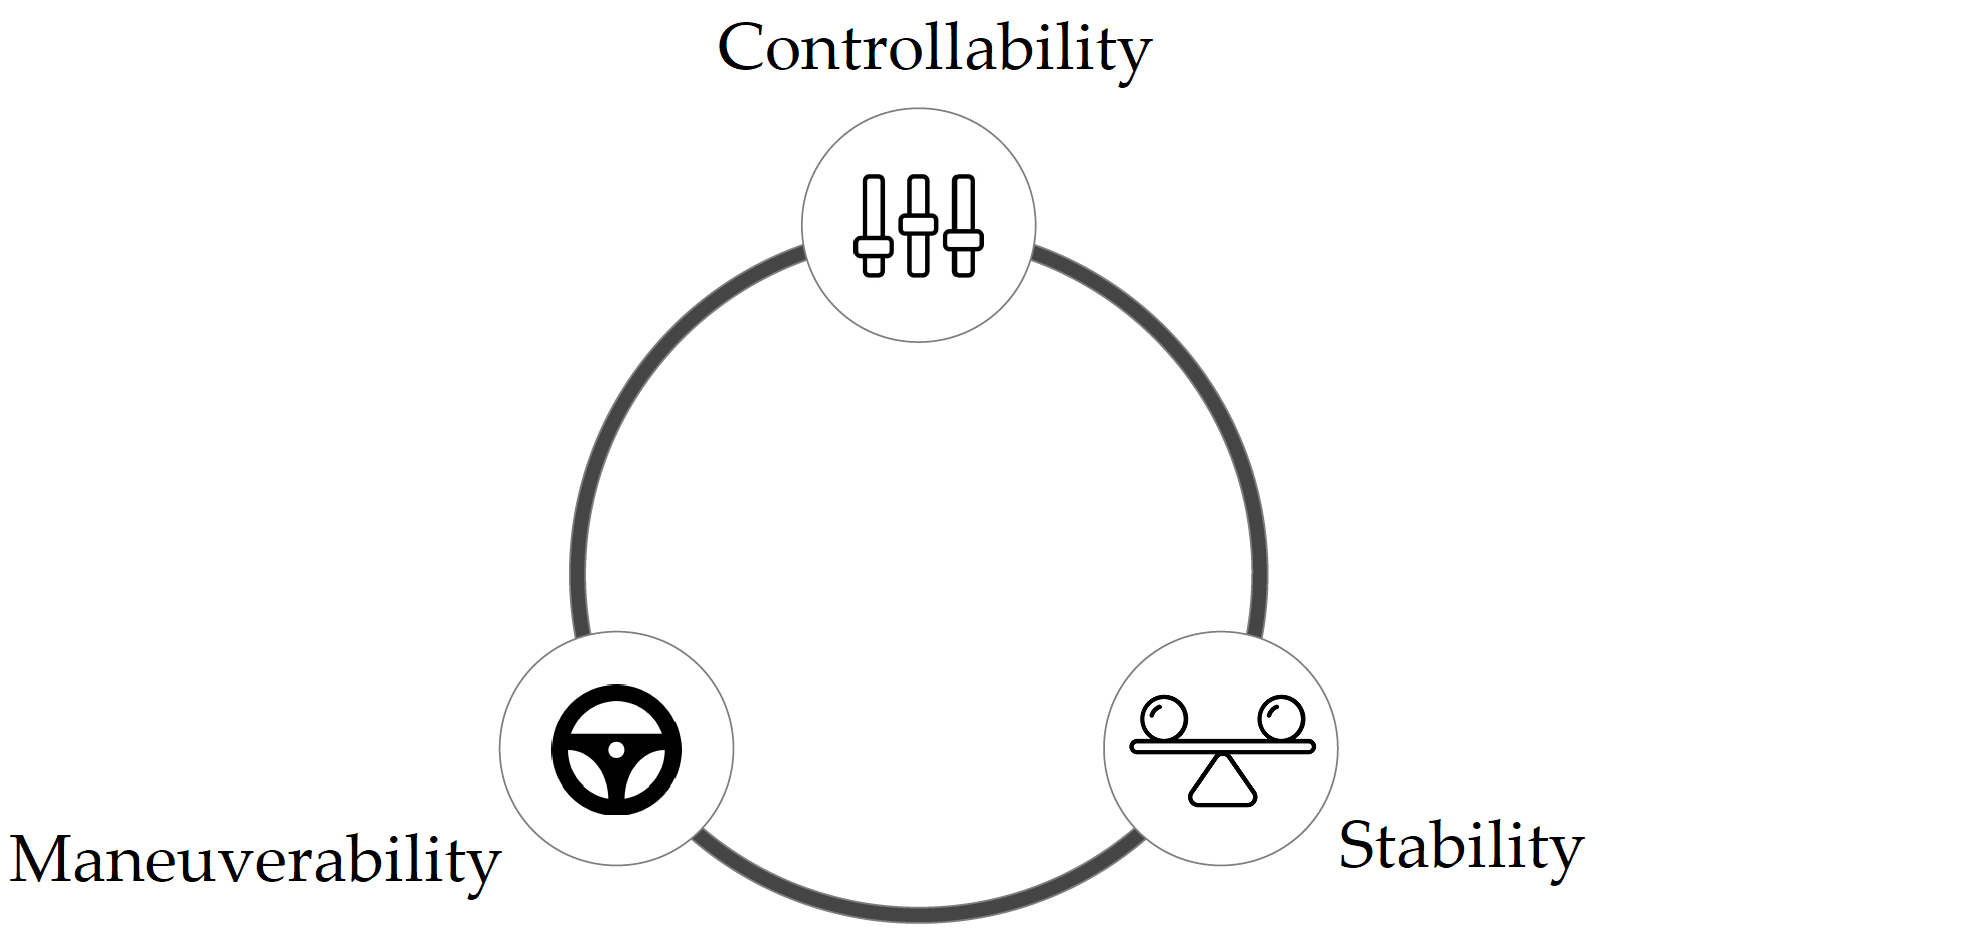
\includegraphics[height=5cm]{figures/triangle.png}
	\label{triangle}
	\caption{Major aspects of wheeled robot design}
\end{figure}

In general, balance is not usually an issue in wheeled robotics as they are designed such a way that the all wheels are in contact with the ground. Having three wheels is sufficient to guarantee the static stability if the center of gravity is within the triangle formed by three contact points. Obviously in case of two wheels, self-balancing is necessary. When more than two wheels are used, once the stability improved by adding more contact possibilites, but also a flexible suspension system is required to allow all wheels to maintain ground contact when the robot moves on uneven terrain. One of the simplest approaches to suspension is to design flexibility into the wheel itself, i.e. applying deformable tire of soft rubber material.

Basically, the maneuverability of a given robot depends on the design, robot configuration and degrees of freedoms of powered wheels. Each wheel type has their advantages and disadvantages that have to be considered before building a mobile robot, we will see the details later. The robot arrangements can be classified into two groups: holonomic and anholonomic. A mechanical system is called anholonomic if in a specific configuration (state) there exists such displacement or rotation that cannot be carried out by means of the combination of possible actuators. A well known example when an automobile cannot move perpendicular to its orientation by powering the wheels because that of the kinematic constrains. On the other hand, some robots are holonomic, in other words omnidirectional, meaning that they can move at any state in any direction along the ground plane (x,y) regardless of the orientation of the robot around its vertical axis. This level of maneuverability requires wheels that can move in more than just one direction, we will see the details later too.

The controllability and maneuverability are usually in an inverse correlation. For example, the omnidirectional designs require more control processing to convert desired rotational and translational velocities to individual wheel commands. In addition, omnidirectional robots need to have more degrees of freedom at the wheel. Controlling an omnidirectional robot for a given direction of moving is a harder task and less accurate compared to less maneuverable designs, e.g. an anholonomic car.

As conclusion, there is no perfect robot configuration that simultaneously maximizes stability, maneuverability, and controllability. For that reason, it is always the designer's task to choose the most appropriate mobile robot configuration considering the constraints originated from the given application. \cite{sieg}


\subsubsection{Wheel design}
The choice of the wheel type has a large effect on the overall kinematics. There are four major wheel classes as shown in figure below.
\begin{figure}[h]
	\centering
	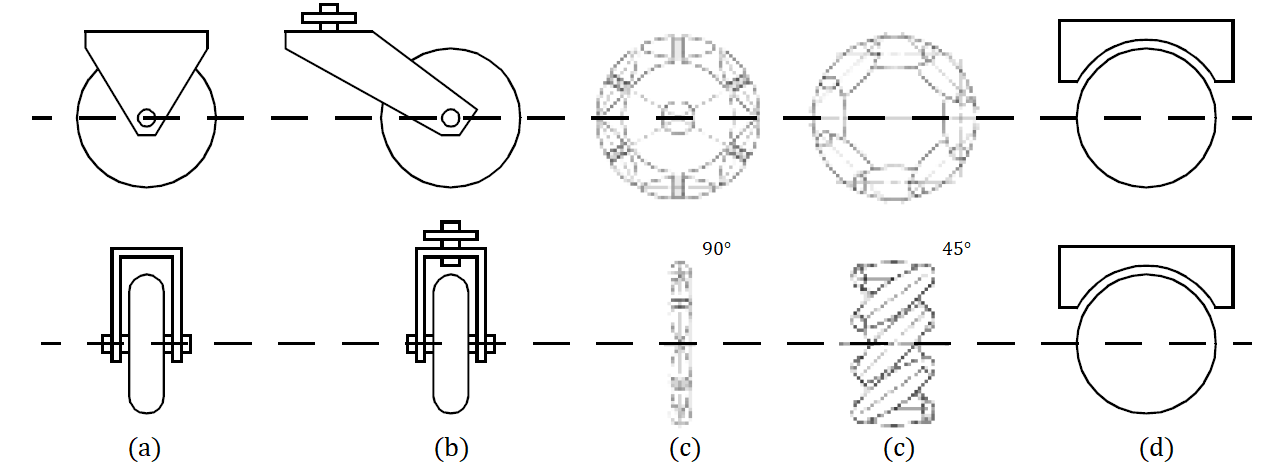
\includegraphics[height=4.5cm]{figures/wheels4.png}
	\label{wheels}
	\caption{Major classes of wheels: 
		(a) Standard wheel, (b) Castor wheel, (c) Swedish wheel (45$^{\circ}$/90$^{\circ}$), (d) Ball wheel \cite{sieg}}
\end{figure}

The standard and castor wheel are mainly one-directional as they have a primary axis around the rotation is possible. These wheels must be steered along a vertical axes to make the case move in a different direction. The castor wheel is special as it can rotate around an offset vertical axis causing an extra torque imparted to the case compared to the standard wheel case where the axes of rotation passes through the contact point. The castor wheels are always used as passive wheel as they can get aligned in the proper direction due to the friction force, i.e. no control is needed. 
Both the Sweedish and the ball wheel are less constrained directionally than the former conventional ones. The Swedish wheel functions such as a normal wheel providing low resistance in another direction as well, i.e. rolling resistance instead of sticking. Small rollers are attached around the circumference that can rotate, thus the static friction is usually not present. The spinning of the circumferential rollers is always passive while the primary axis is the only powered joint. Eventually, although the wheel can be driven along only the principal axis, the wheel can move along almost any trajectory. The spherical wheel is a truly holonomic wheel, often designed so that it may be actively powered to spin along any direction.

\subsubsection{Wheel configurations}
\paragraph{Holonomic robots}
%In practical applications, holonomic systems are less present in overall due %to higher prices and mechanical complexity, moreover dead reckoning by means %of odometry is quite inaccurate. However they \cite{rirt}\\[10pt]
\noindent \textbf{Three wheeled omnidirectional mobile robot} \\
The mechanically simplest holonomic robot is three-wheeled omnidirectional configuration. At least three independently driven wheels are needed to be able to move in any direction $(x,y,\varphi)$ in ground plane at any time, i.e. to have 3 degrees of freedom.
\begin{figure}[htb!]
	\centering
	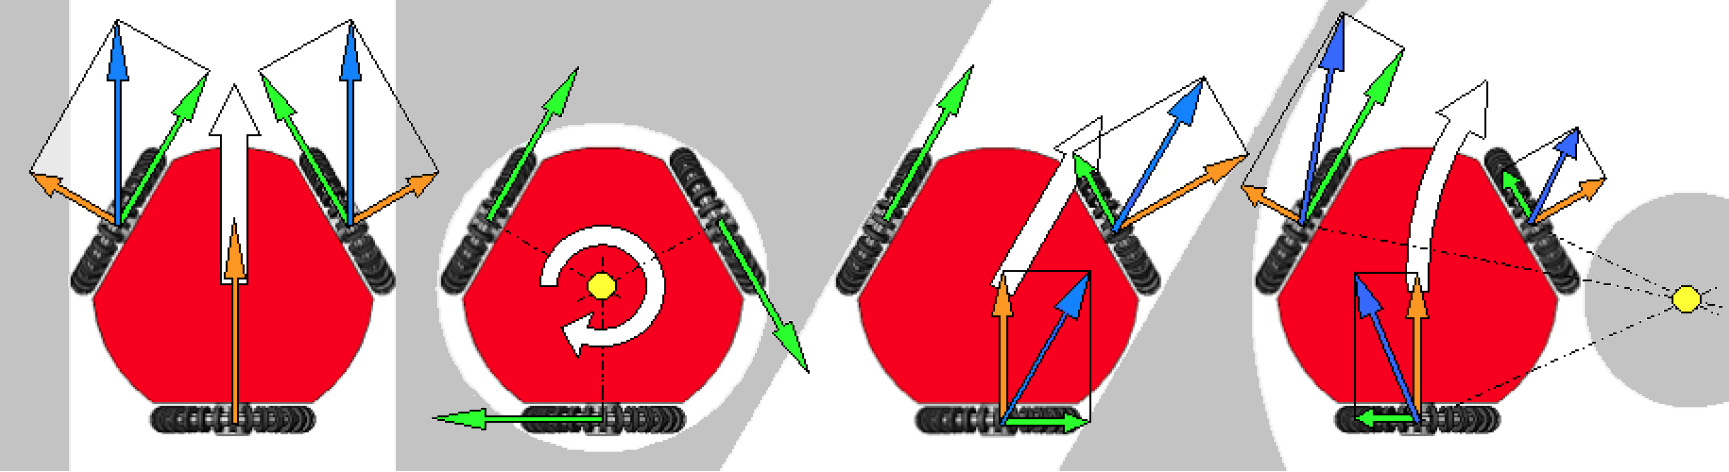
\includegraphics[width=15cm]{figures/omniconfig.png}
	\caption{Three-wheeled omnidirectional drive configuration (blue: common velocity vector of the entire robot; 
		green: speed of the wheel around the primary axis (active wheel speed), orange: speed of passive rollers (passive wheel speed), the resultant velocity is the sum of the active and passive velocity vector; white colored are is where the robot moves with the given velocity configurations \cite{rirt}}
	\label{omniconfig}
\end{figure}

The resultant velocity vectors in terms of wheel velocities can be seen in Figure \ref{omniconfig}. The blue wheel velocity vectors can have lateral component, i.e. the wheels have to be able to move parallel to their primary axes. This kind of configuration needs the previously mentioned Swedish wheels or spherical wheels, i.e. holonomic wheels. 
In addition, also four wheels or even more can be built-in, but in this case it can occur that the wheels drive each other in opposite direction, moreover more than three contact point does not guarantee the proper contact of each wheels with the ground as slippage can happen more easily.\\[10pt]
\noindent \textbf{Omnidirectional robot with four Swedish wheel} \\
Four-wheeled arrangement with 45$^{\circ}$ Swedish wheels, each driven by a separate motor, has been used in several research and industrial projects. A good example is Uranus that can rotate and translate independently without any constraints with the help of omnidirectional wheels.
\begin{figure}[htb!]
	\centering
	\minipage{0.47\textwidth}
	\centering
	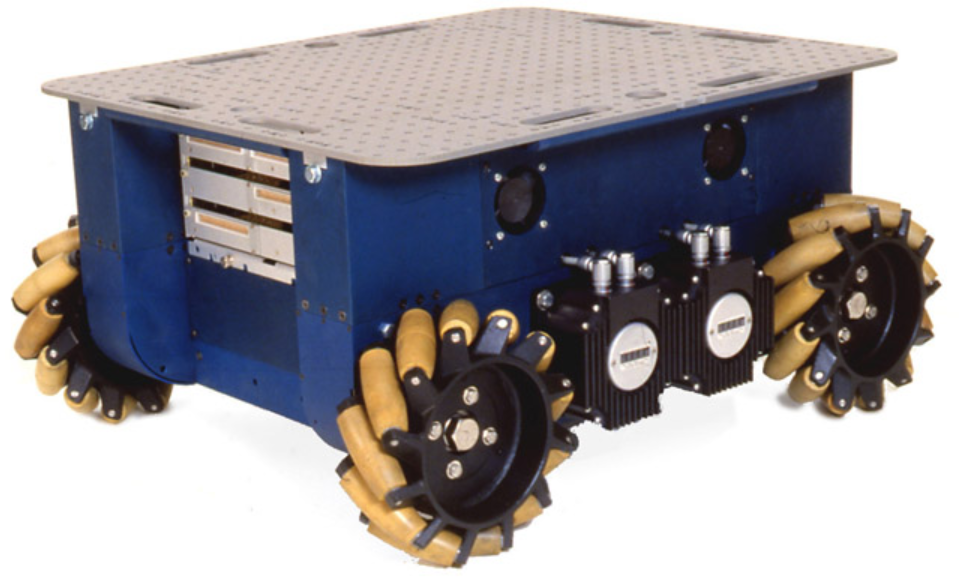
\includegraphics[height=3cm]{figures/uranus}
	\caption{Carnegie Mellon Uranus robot}
	\endminipage\hfill
	\minipage{0.53\textwidth}
	\centering
	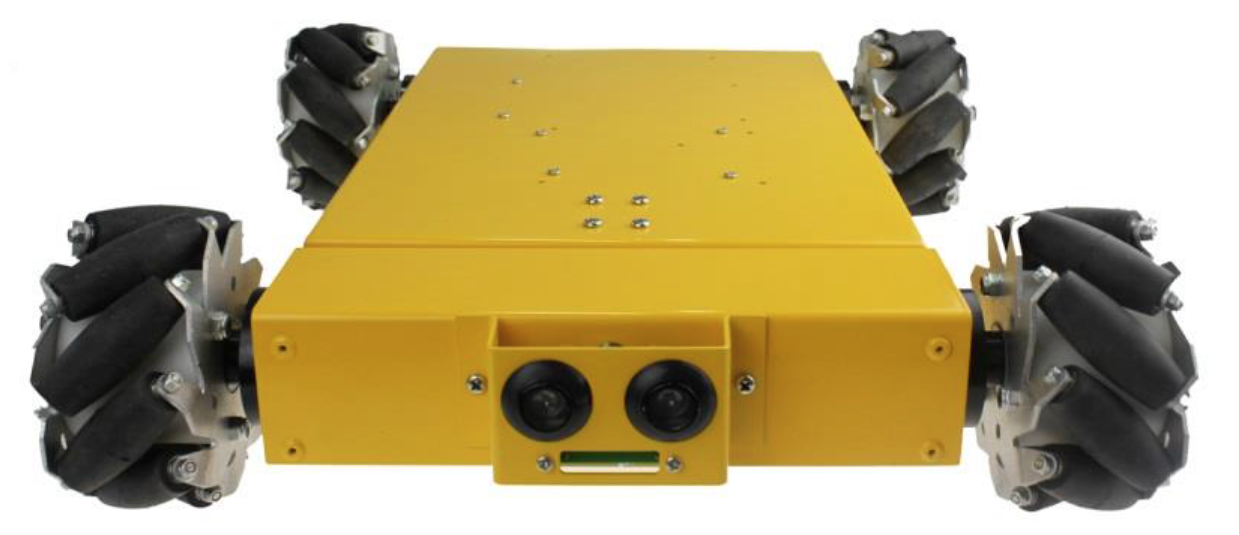
\includegraphics[height=3cm]{figures/mecanum}
	\caption{Mecanum AB robot}
	\label{mecanum}
	\endminipage\hfill
\end{figure} \\
When all four wheels spin in the same direction, the robot moves longitudinally in a straight line forward or backward, accordingly. When one diagonal pair of wheels spin in the same direction and the other diagonal pair of wheels spin in the opposite direction, the robot moves purely laterally. The simultaneous spin can be achieved if the wheels on left side are driven in forward or backward while the wheels on the other side are driven the corresponding opposite direction. As it was discussed earlier, this four-wheel arrangement is not minimal in terms of control, stability and maneuverability, but preferred over three-wheeled configuration for higher capacity and stability reasons. \\[10pt]
Main disadvantages of omnidirectional configurations include the complexity of control because of the more complicated processing of wheel velocities. For instance, the Swedish wheels have a set of free rollers along the wheel perimeter adding extra degrees of freedom, i.e. translation in the lateral direction. Furthermore, due to these rollers the wheel perimeter is not a perfect circle, thus accuracy of dead-reckoning based on counting the number of rotations might be inaccurate. The rollers can also cause slippage, thus accumulation of displacement errors. \cite{sieg}

\paragraph{Anholonomic robots}
The non holonomic wheeled robot configurations are more widely spread, e.g. automatic wheelchairs or robot cars. The most common choice of indoor robotics is the well-known two-wheel differential drive due to its simplicity beside acceptable maneuverability, only slightly inferior to omnidirectional drives. In optimal configuration the two wheels are arranged symmetrically, thus the robot can spin around the center point of the case without changing its location. One or two additional ground points, e.g. non driven castor wheel(s), are usually added to gain stability. 
\begin{figure}[htb!]
	\centering
	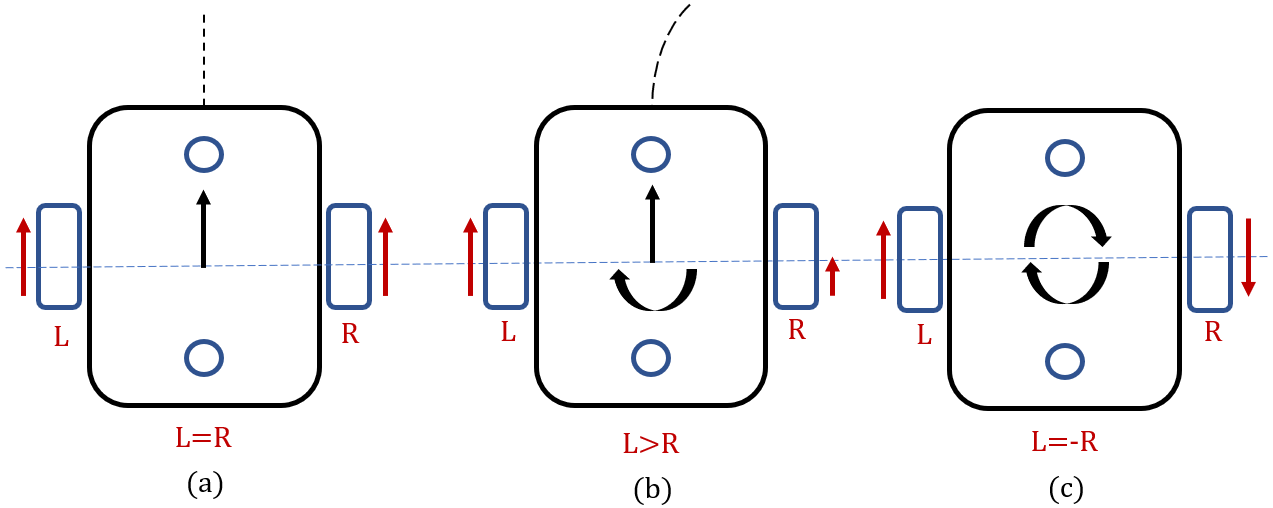
\includegraphics[height=6cm]{figures/differential.png}
	\caption{Two-wheeled differential drive configuration; the resultant kinematic state (linear and angular velocity - black) depends on the ratio of the two driven wheel velocities (red); (a) moving along a straight line case; (b) moving along a curved line case; (c) pure spinning at a given position case;}
	\label{differential}
\end{figure}

In such robotics, motion in a particular direction may initially require a rotational motion to be able to change the position along straight movements. Two wheel differential drive is not clearly omnidirectional but motion can be decomposed 
into distinct rotation and displacement according to the given order. One can say, that it has two and a half degrees of freedom compared to three wheeled omnidirectional configurations that have three whole degrees of freedom.
The advantages include easy maneuverability, simple construction as only two motors and two conventional wheels needed. Also two wheels can be enough, but in this case self-balancing control has to be attached, in general castor wheels are preferred. The disadvantages of this configuration are lower lateral stability at higher speed turns, sensitivity to terrain roughness, furthermore if the axes of the two wheels are not coincident, the sliding of the wheels will occur. \cite{rirt}

Similarly to automobiles, remarkable part of the four-wheel robots uses the Ackerman steering geometry. It is a way of geometric arrangement of linkages in the steering of a vehicle  which is designed such a way that the inner and outer wheel of a turn can move along circles of different suitable curvatures. 
\begin{figure}[htb!]
	\centering
	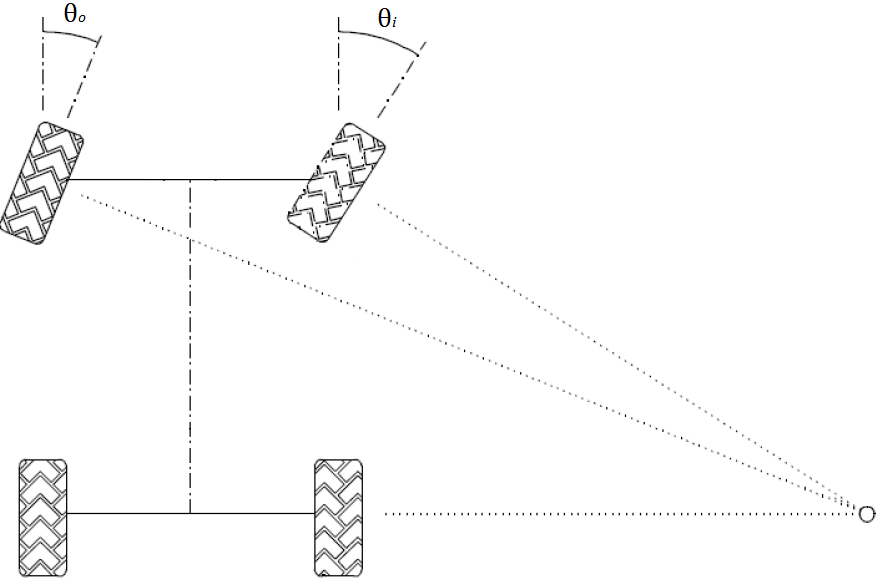
\includegraphics[height=6cm]{figures/ackerman2.png}
	\caption{Ackerman steering arrangement \cite{rirt}}
	\label{ackerman2}
\end{figure}
It is important that ${\theta}_i$ and ${\theta}_o$ angles cannot be the same whereas in that case the constant sliding of the wheels would be inevitable. In addition, the rear wheels also have to be tuned to spin with different appropriate velocities as they move along different trajectories. As Figure \ref{ackerman2} depicts, such a vehicle typically has a turning diameter that is larger than itself, thus to move sideways requires a parking maneuver consisting of repeated changes in forward and backward direction. In addition, the limited maneuverability of Ackerman steering has an important advantage, i.e. its directionality and steering geometry provide a
very good lateral stability in high-speed turns. Furthermore, it is much more easier to go straight simply by locking the steerable wheels and driving the drive wheels compared to the omnidirectional configurations where permanent control is always needed. \cite{rirt} \cite{sieg}

Multi-degree-of-freedom robots have more than the needed three degrees of freedom. They have enhanced maneuverability, but as a result of the over determined arrangement the slippage free control is more challenging at the same time. The main application scope are mostly the navigation on uneven terrains, e.g. military applications or moon rovers. The position tracking is impossible by odometry, thus external sensors are essentially needed. 

\begin{figure}[htb!]
	\centering
	\minipage{0.48\textwidth}
	\centering
	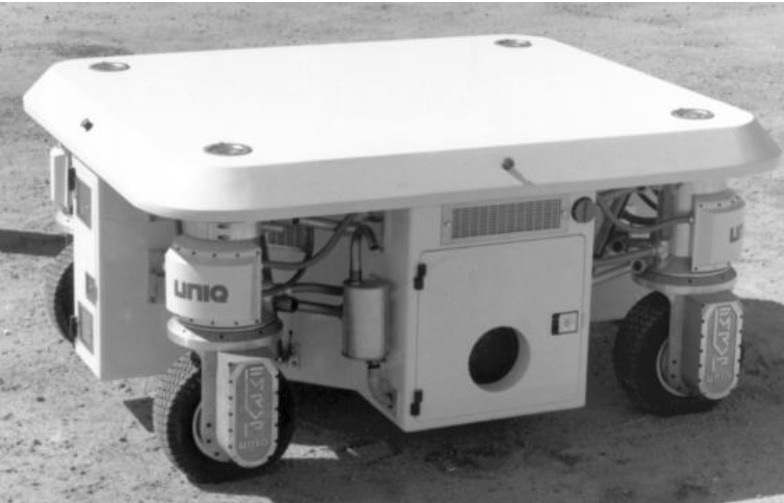
\includegraphics[height=5cm]{figures/uniq.png}
	\caption{UNIQ: 8 DOF mobile robot (each wheel is driven and steerable) \cite{rirt}}
	\endminipage\hfill
	\minipage{0.48\textwidth}
	\centering
	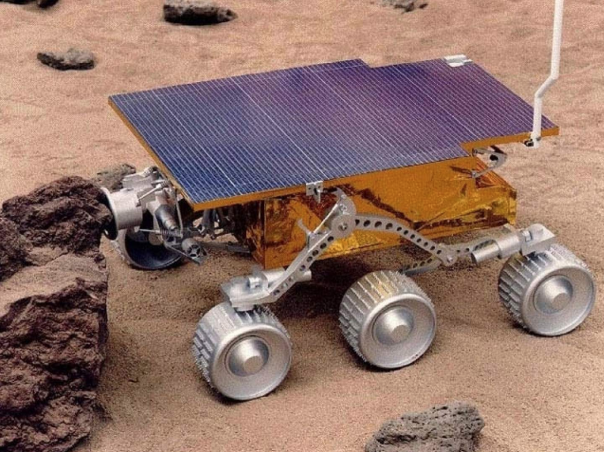
\includegraphics[height=5cm]{figures/rover.png}
	\caption{Sojourner: Mars rover of NASA \cite{rirt}}
	\label{mecanum}
	\endminipage\hfill
\end{figure}

\newpage
\section{The Hardware Application}
\subsection{Selecting a mobile robot configuration}
In previous chapters the basic features of mobile robots and some real life application were presented. This final project basically aims at designing an autonomous transport robot to investigate its control and possible parameter estimation problems. Real world transport robots are usually capable to navigate along prescribed path, monitor their environment to handle unexpected obstacles, interact with the packages autonomously and communicate with users surrounding them. These are the most necessary features that are really needed during operation which have been mostly implemented in the past.

The development of kinematic and dynamic properties have been taken less attention so far, therefore this field can contain remarkable development potential in my opinion. The transport robots in industrial application are designed such a way that during their movement they will not likely face issues regarding the stability because they move along
high radius path with low speed and accelerate moderately. In other words, a compromise is made between the configuration costs and the productivity, between the security and effectiveness. Sooner or later, the demand for a more dynamic, faster and smoother operation of transport robots can come into being just like in automotive industry. The problem can be more complex as well in certain situations. For instance, a transport robot operating in a plant that carries loads with different properties such as mass, moment of inertia or height would face a more challenging situation in dynamic stability point of view than a car with more or less known and constant physical parameters.

To select a mobile configuration, the general purpose, working environment and concept of the robot have to be defined. Based on real life experiences and possible future application needs, this study will focus on designing a transport robot which would operate in a laboratory carrying different shaped and weighted loads. Instead focusing on navigation, i.e. dead-reckoning, route planning and obstacle avoiding, the control of dynamic behavior is to be examined in details.  As it was mentioned, the lower level issues will be in focus instead of the higher level ones. In  a former project in a similar way, the focus was firstly on lower level problems, then the robot platform after some further developments was able to participate in a robot football match of the Indonesia Robot Contest. \cite{robot_focis}. Another application of a four wheeled omnidirectional vehicle was a development of an algorithm to calculate near-optimal minimum time trajectories which can be used as part of a high-level path planner. \cite{robot_focis_2} In this work also detailed analysis of vehicle dynamics were carried out.

Beside the technological aspects also the practicability and costs have to be considered since the building of the mobile robot configuration is also the part of my thesis. The most important aspect of a study of such an advanced moving transport robot is the maneuverability. In terms of maneuverability, the omnidirectional robots show the best performance. Choosing a three-wheeled omnidirectional mobile robot configuration can be regarded the optimal choice. The controllability is more complex compared to anholonomic robots, but with the choice of minimum number of three wheels it is still an easily handleable design challenge. Application of more wheels could give more controllability which would be favored, e.g. TUG is also four wheel driven omnidirectional configuration. However, it would make some additional issues appear such increased slip danger and more complex controllability. Compared to anholonomic configuration, the holonomic configurations are less stable as mentioned before, but it can be regarded as an advantage in this case, because this study is willing to deal with stability issues, thus the main objective is to examine the behavior of the system near stability and provide parameter estimation methods to avoid it. In other words, the possibility of demonstration of the problem to solve it is more important than simply avoiding it.
In other words, a transport robot might be preferred over others if it can be as stable as possible without loosing any maneuverability skill. For an omnidirectional drive configuration special wheels of higher price are needed, thus the three-wheeled configuration is optimal from economic point of view as well compared to more wheeled omnidirectional robots.

\subsection{The Hardware}
The realised mobile robot was built from scratch ordering its part from different sources. In this chapter, the components of the mobile robot platform are presented.
\begin{itemize}
{\small 	\item Triangle-shaped cases (3 elements): makes structural integrity by holding the machine components; more levels are needed in order to have place for a package too.
	\item Separate DC motors for all wheels with hall sensors: electric energy to kinetic energy conversion during locomotion; for controllability magnetic encoders are attached.
	\item L298N Motor Drivers: power electronic module which drives the motors.
	\item Microcontroller (Arduino Mega 2560): makes the calculations in order to operate the whole as a system, communicates with all devices.
	\item Bluetooth Module (HC-05): gives the possibility of wireless serial communication
	\item Step-up and voltage regulator modules: electronic modules that helps to connect certain parts of the the electronic circuit
	\item Battery: energy storage; provides the energy needed for the operation of electronics and the motors.}
\end{itemize}
\begin{figure}[htb!]
	\centering
	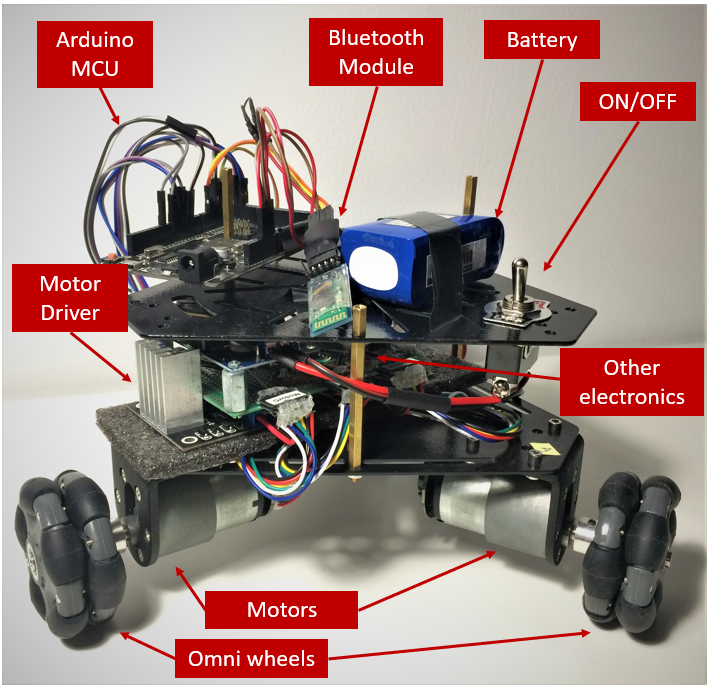
\includegraphics[width=0.6\textwidth]{figures/robot_platform_1.png}
	\caption{Robot platform: Three-wheeled omnidirectional robot}
	\label{robot_platform_1}
\end{figure}
\newpage
\subsubsection{Platform base}
In Figure \ref{case_1} a photo of the assembled robot case is shown. The DC motors are attached to the case using L shaped brackets. One, two or three levels can be built from triangle shaped metal sheets which have a black electrically insulating coating. The main purpose of the frame beside making connection between the wheels is to provide a safe place for all components of the robot, such as the electronic modules. Using the free center hole in the most upper level, a threaded rod can be attached to the case to provide a place for mounting additional payloads demonstrating the weight of an arbitrary package. The side size is 145mm, thus common wheel circle has a radius of 0.12m. The weight of the case, motors and the wheels is about 1.3kg.
\begin{figure}[htb!]
	\centering
	\minipage{0.5\textwidth}
	\centering
	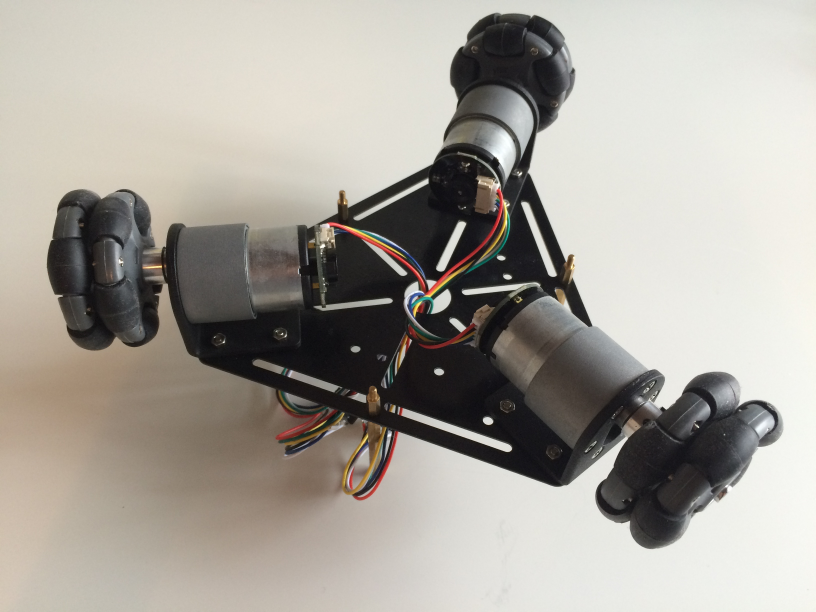
\includegraphics[width=7cm]{figures/case_1}
	\caption{Robot case (bottom)}
	\label{case_1}
	\endminipage\hfill
	\minipage{0.5\textwidth}
	\centering
	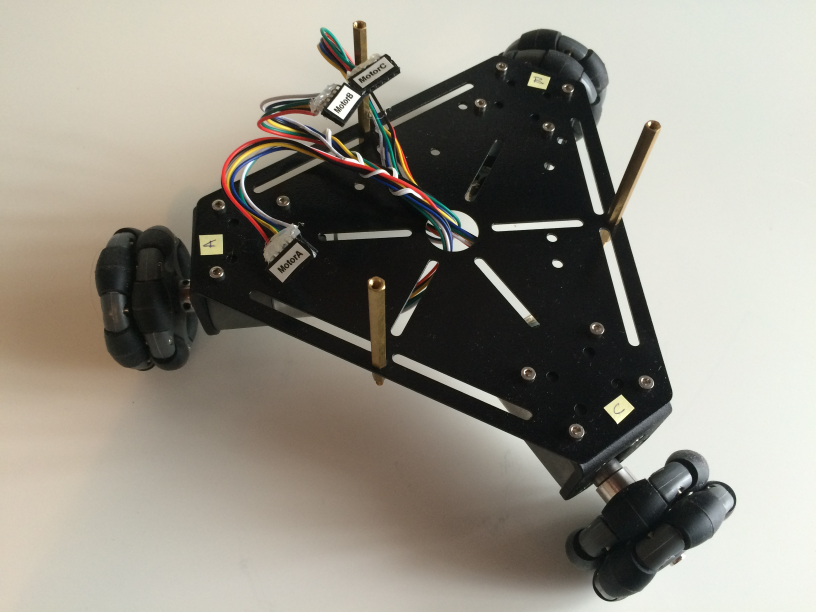
\includegraphics[width=7cm]{figures/case_2}
	\caption{Robot case (top)}
	\label{case_2}
	\endminipage\hfill
\end{figure}
\subsubsection{Omni wheel}
In order to fulfill the maneuverability demand, a configuration with omni wheels was looked for. As it was mentioned, the omni wheels are like regular ones which can roll around their axis but with additional passive rollers along its circumference which allows the wheel itself to move in the lateral direction as well. Because of the additional rollers, the contact point(s) (mainly there are two of them even if rigid wheels are considered) will not be always under the wheel center, e.g. when shifting between rollers occurs. As a result of that, the movement on flat surfaces will be less smooth compared to conventional wheels. Applying more rows of rollers, the uneven rolling characteristic (transition between passive rollers) can be improved. However, the contact point changes in the lateral direction too. \cite{owp1}
\begin{figure}[htb!]
	\centering
	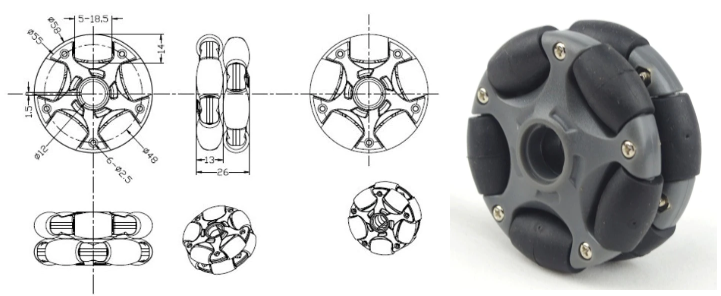
\includegraphics[width=10cm]{figures/omni_wheel.png}
	\caption{Omni wheel construction}
	\label{omni_wheel}
\end{figure}
The ordered wheel is shown in Figure \ref{omni_wheel}. Such a wheel is made of plastic having maximum nominal load capacity of 3kg and 58mm diameter. It can be connected to the shaft of a DC Motor using a coupling hub and screws.
\subsubsection{Gear Motor}
In mobile robotics, the DC (direct current) motor is a general choice for actuation purposes. The points which are to be considered are as follows:
\begin{itemize}
	\item Its nominal operating voltage and the current consumption which is needed during the possible operating states. The energy source and the electronic devices have to be able to provide the electrical energy in the given needed form.
	\item Motor torque has to be in match with the inertias of the robot configuration.
	\item Motor speed has to be in match with the demands regarding the demanded locomotion speed of the case.
\end{itemize}
At the given scale, the DC motors are more commonly brushed permanent magnet type. They run at quite high speed about 10,000-12,000 RPM having a little torque.\cite{dc_motor_5} For a robot application, it is too fast and the torque is too little, therefore motors with gearbox attachment are needed. The gearbox is a set of gears containing several stages to increase the motor torque at the cost of the shaft speed. What is more, also a lower resolution encoder is enough since that of resolution is also increased. The selected DC gear motors are represented in Figure \ref{gear_motor1}.
\begin{table}[htb!]
	\begin{tabular}{lc}
		\hline
		\multicolumn{2}{l}{DC Gear Motor Datasheet}                                                   \\ \hline
		Rated voltage                      & DC 12.0 V                                                \\
		No-load speed parameter            & 107 {[}RPM{]}- 0.15 {[}A{]}                              \\
		Maximum efficiency point parameter & 85 {[}RPM{]} - 0.6 {[}A{]} - 0.42 {[}Nm{]} - 3.8 {[}W{]} \\
		Maximum power point parameter      & 52 {[}RPM{]} - 1.2 {[}A{]} - 0.98 {[}Nm{]} - 6.0 {[}W{]} \\
		Blocking point parameter           & 3.4 {[}A{]} - 1.96 {[}Nm{]}                              \\
		Gear ratio                         & 1:90                                                     \\
		Encoder resolution                 & 1:11                                                    
	\end{tabular}
	\label{mct}
	\caption{Motor characteristics}
\end{table}
\begin{figure}[htb!]
	\centering
	\minipage{0.5\textwidth}
	\centering
	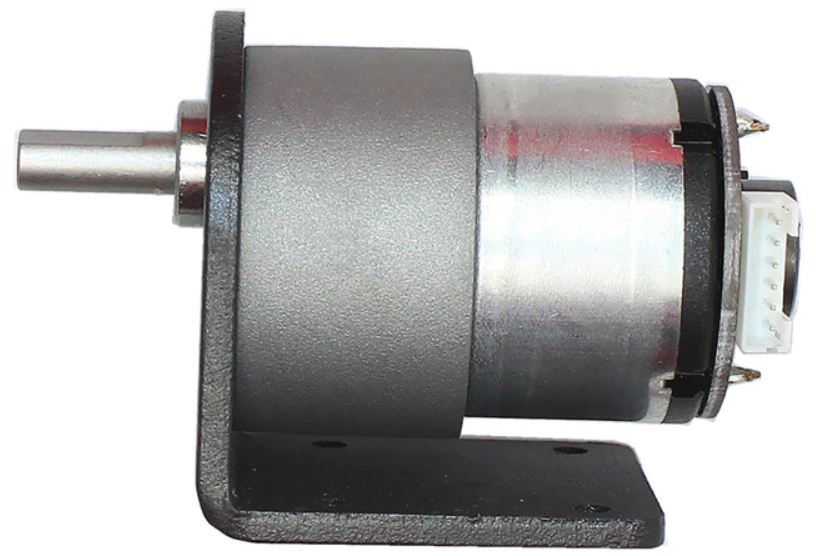
\includegraphics[width=6cm]{figures/gear_motor1}
	\caption{Selected gear motor}
	\label{gear_motor1}
	\endminipage\hfill
	\minipage{0.5\textwidth}
	\centering
	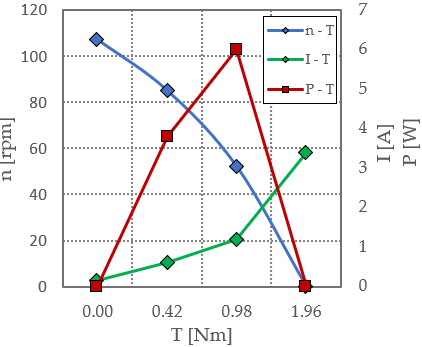
\includegraphics[width=8cm]{figures/gear_motor2}
	\caption{Gear motor characteristics}
	\label{gear_motor2}
	\endminipage\hfill
\end{figure}

The supplier provided the nominal values of specific working points which are shown in Figure \ref{gear_motor2} and listed in Table 3.1.
The motor is equipped by magnetic quadrature encoders in order to allow to count the revolutions. There are two Hall-effect sensor which are able to detect the changes of the magnetic field caused by ferromagnetic magnets attached to a gear. If a magnet passes near in front of the sensor, the magnetic field will be changed which will cause the output of the sensor to either go high or low in terms of voltage. The frequency of the generated square wave will be proportional with rotational speed of the shaft. In order to identify the direction of the rotation (clockwise or counter-clockwise) a second sensor is attached to motor. Eventually, the encoder provides $2 \times 2 \times 11 = 44$ counts per revolution considering that the observed gear has 11 magnets, two hall sensors are present and both rising and falling edge are counted. In addition, the motor has a gearbox with a ratio of 1:90, thus the Hall-effect sensor generated $44 \times 90 = 3960$ counts per revolution. Therefore the accuracy in theory is about $0.09^{\circ}$ which is high enough for an accurate speed calculation.

\subsubsection{Electronics}
A RobotDyn Mega 2560 board with an ATmega2560 (16Mhz) microcontroller was chosen which is a cheap version of the original Arduino board having the same capabilities and compatibilities. Arduino is an open-source electronics platform including easy-to-use hardware and software. \cite{arduino} The programming language is based on C++, the Arduino library is well-documented, widely used and easy to learn. There are several boards compatible with Arduino at lower prices as well. The Mega actually was chosen for its increased number of pins compared to base models such as Uno.
\begin{figure}[htb!]
	\centering
	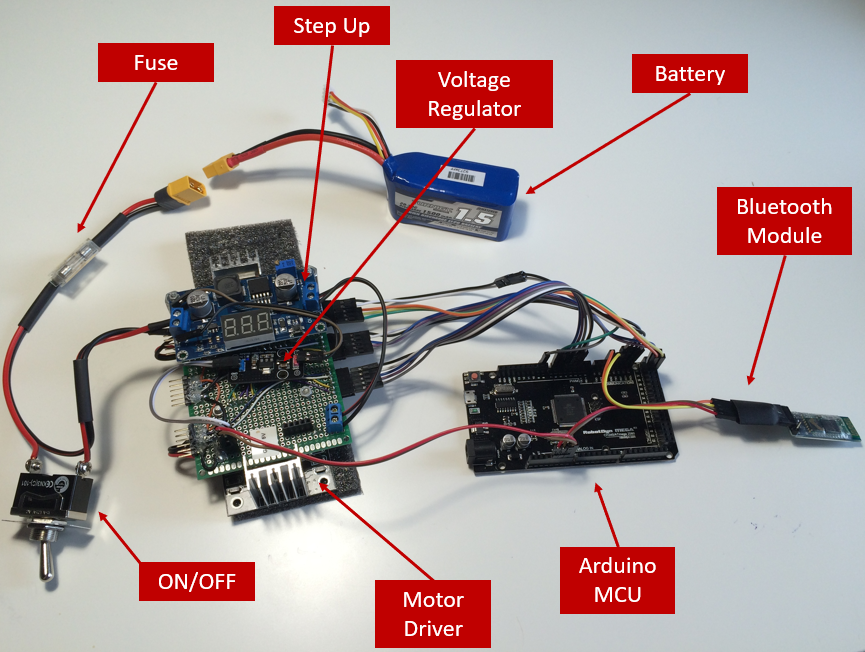
\includegraphics[width=\textwidth]{figures/electronics.png}
	\label{electronics}
	\caption{Electronics of the robot platform}
\end{figure}

Considering the rated voltage of the DC motors and other aspects such as space and performance, 3-celled LiPo (lithium polimer) with 3x3.7V rated voltage battery was chosen to power the mobile robot. This type is widely used for its good capacity over weight ratio, high current supply capability and fast charging. The main disadvantage of this kind of batteries that they can flame up in case of short circuit caused by a serious mechanical damage or some kind of abnormal use. For safety reason, an electrical fuse was added to protect the battery and also the electronic circuits from operating under overcurrent. 

Generally, two voltage levels have to be provided: a logic circuit with 5V and a power circuit that provides 12V at motor pins, in addition, a common ground has to be formed. This separation is essentially needed since the microcontroller board works with an operating voltage of 5V and also other electronic circuits can operate on that voltage level, futhermore the board can provide maximum of 40mA at a single pin which would not be sufficient to drive the motors. The board has an own voltage regulator but it is recommended to power with a voltage less than 12V, thus for driving the motor a higher voltage circuit is essential. \cite{arduino} 

A DC motor can be switched on/off using a MOSFET transistor connecting a digital output of the board to its gate and providing high or low voltage, thus opening or closing it. The technique makes it possible to connect higher voltage and current to the motor directly from the power source using a programmable electronic device. If constant voltage is supplied, a DC motor will spin as fast as it can in accordance with inner and outer resistance type load which characteristic is shown in Figure \ref{gear_motor2}. The most efficient way to control the speed of a permanent magnet type DC motor is using the PWM technique. The pulse-width modulation (PWM) technique gives an alternating voltage signal with a given period of time which can be only zero or high voltage values. The percentage of the time period when the voltage level is high called the duty cycle. If a pwm signal with a sufficiently high frequency is generated, the motor with a much larger time constant will sense as if it was a direct voltage input signal with a given average voltage value. This is because of the fact that a motor has inertias ($J,L$) and frictional losses, therefore it takes time to react to sudden changes and it will filter the PWM command resulting in an averaged signal. \cite{dc_motor_3} \cite{dc_motor_4} The average voltage value will be proportional with the duty cycle of the PWM signal. Such an alternating signal, e.g. a square-wave can be generated with some of the digital output pins of the arduino board. Unfortunately, for controlling the direction of rotation speed further components are needed. The motor will spin in the reverse direction if the polarity of the voltage, thus direction of the armature current is switched. A general solution for that is to applying H-Bridge circuit which contains four switches, e.g. transistors, and the motor itself. By working the appropriate switches, the direction of the current flow can be changed. \cite{howtomech}

The so called motor divers have these functionalities, in my case the usually used L298N driver was chosen as it is cheap and it can do what is needed. The main disadvantage of such drives that they cause a substantial voltage drop, i.e. 1-2V in case of 12V supply voltage which will result in a lower motor speed. To handle this problem, an additional step-up converter was attached just after the battery to have a higher supply voltage. After some  application of trial and error method, it was found that if the supply voltage is stepped up to 13.4V, then the motors will get 12V at maximum duty cycle of the pwm signal. With this extra step up module, also the voltage drop of the battery (when it goes dead) can be handled and kept on a constant voltage with a higher supply current. The logic voltage high level (5V) is produced by a voltage regulator connected after the step-up module. The logic voltage level has to be wired into all the devices, thus the motor encoders, microcontroller unit (MCU) and motor drivers (L298N) together with the common ground. The motor driver has to be connected also with the input voltage. The pwm signals are provided by specific pwm capable output pins of the board which have to be connected to the Enable pins of the drivers. Additionally, two digital pins have to connected to the drivers which control the rotational direction of the motors. The motor encoders has two pins called CH1, CH2 which have to be connected to the special interrupt capable pins of the MCU. The interrupt technique guarantees to catch all the pulsed generated by the encoders. If a rising or a falling edge is sensed, then the main loop is interrupted while a predefined so called Interrupt Service Routine (ISR) is called and processed. Once it is finished, the main loop can continue. 

In order to be able to communicate wireless with robot, a bluetooth module (HC-05) was used by which serial communication could be realized. The serial communication is a protocol of a process of sending one bit data at a frequency sequentially over a communication channel. For instance, the Arduino board can communicate with the computer via an USB type cable using the serial communication protocol, e.g. when the code is uploading or when commands are sent from the board to the pc or vice versa. The pins for serial communication are denoted as RX (Receiving) and TX(Transferring) letters, the USB connection is connected to RX1,TX1 serial channel on the Mega. In order to avoid the collision of communication of the bluetooth module and the USB port if both are in use at same time, the BT module was connected to the RX2,TX2 channel.

Using a third-party application called \textit{Joystick bluetooth Commander} on android mobile platform the robot could be remote controlled via bluetooth serial communication.
\begin{figure}[htb!]
	\centering
	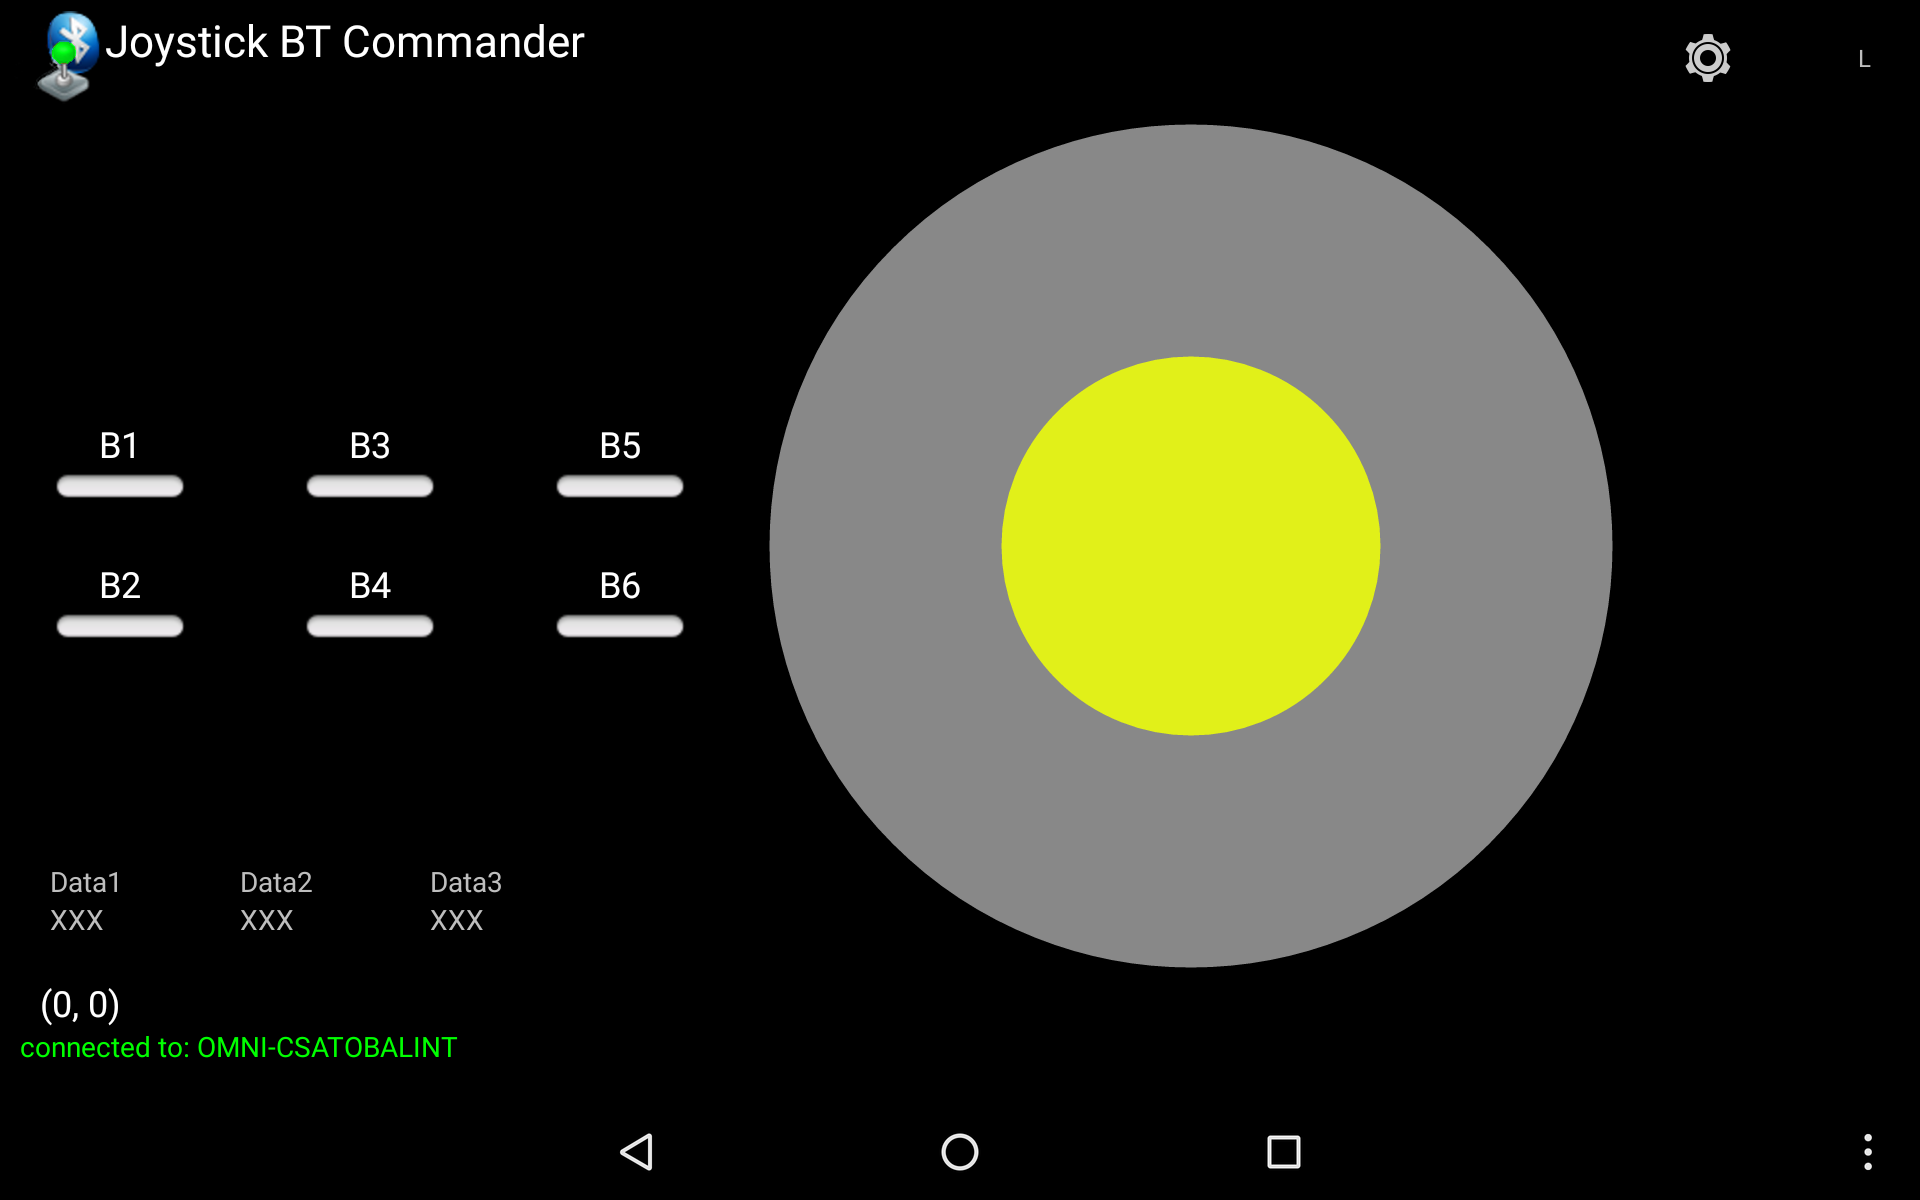
\includegraphics[width=\textwidth]{figures/jybt.png}
	\label{electronics}
	\caption{Joystick bluetooth Commander dashboard}
\end{figure}
This is an open-source software code for which several examples were provided, also an arduino code that handles whether a button is pressed or move commands are sent by the analog joystick.
\newpage
\subsubsection{Schematic diagram of the electronics}
\begin{figure}[htb!]
	\centering
	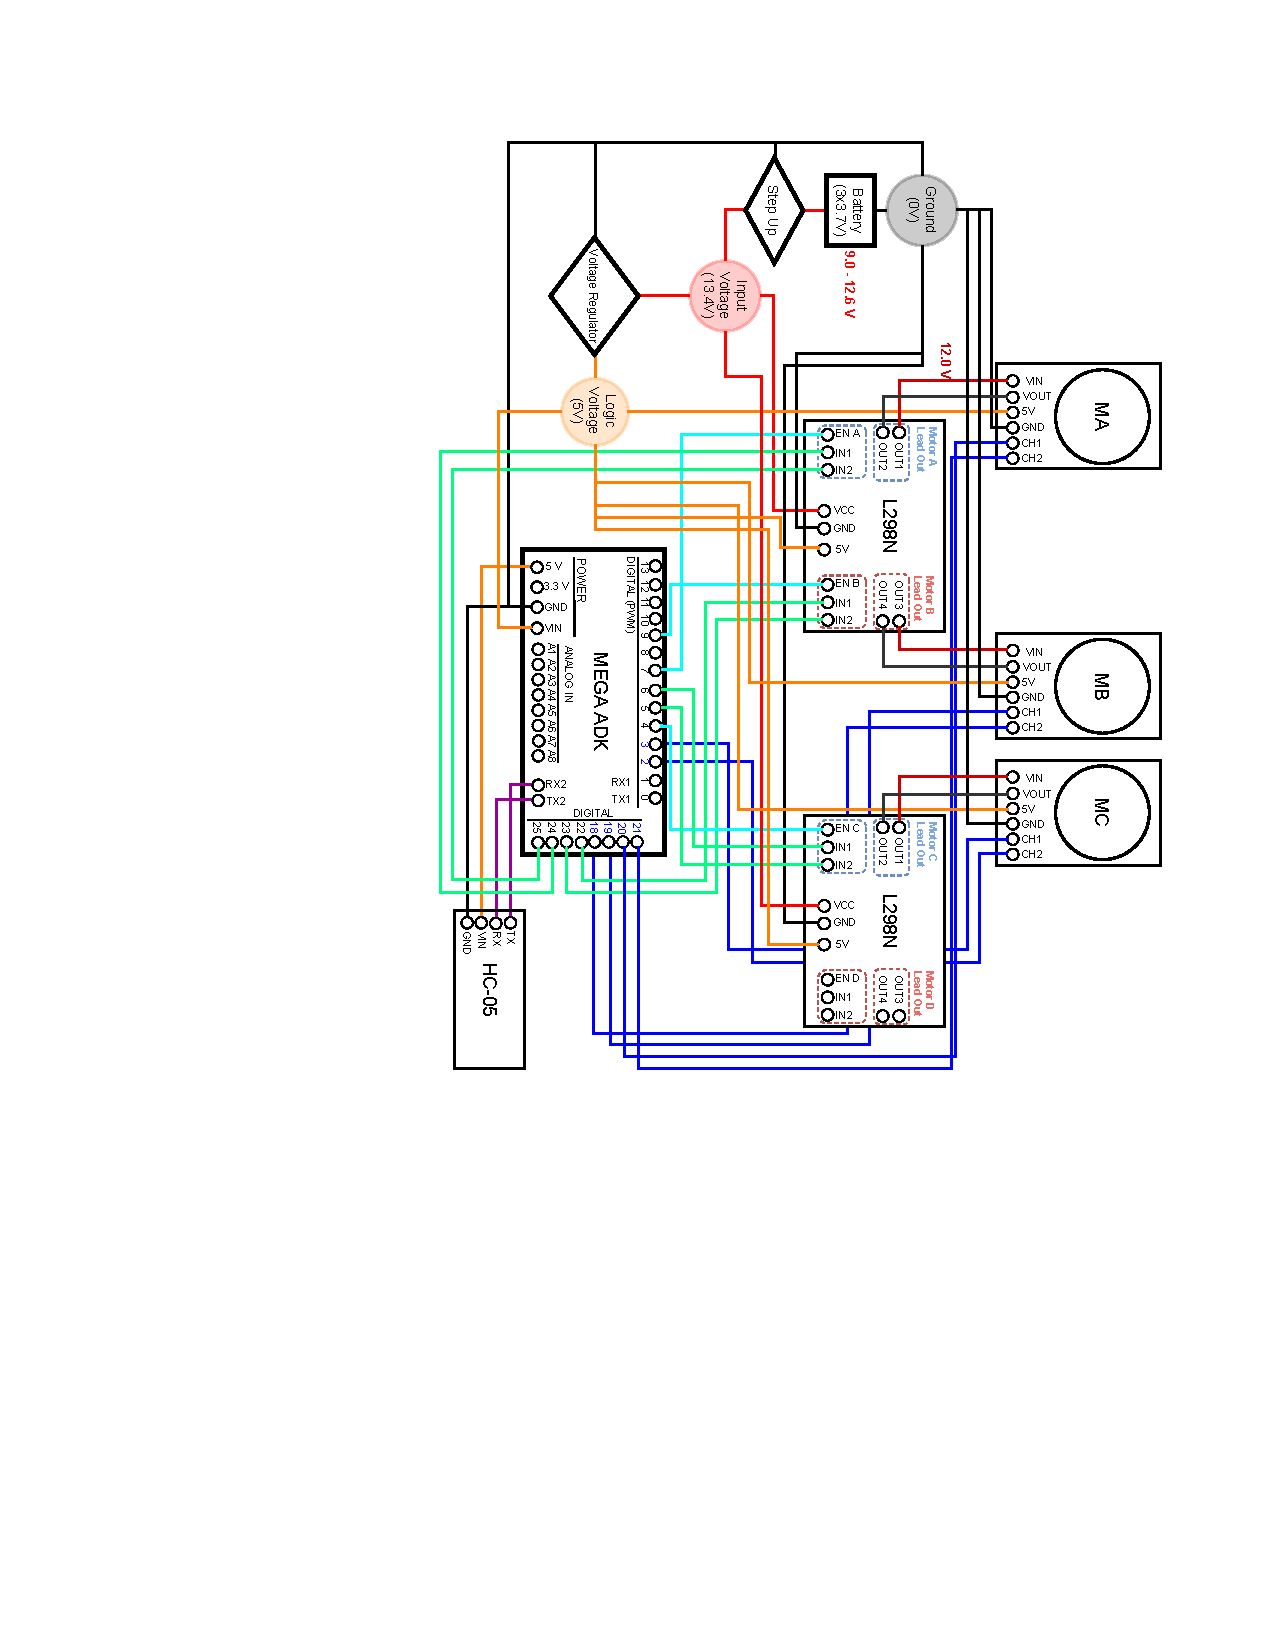
\includegraphics[width=\textwidth]{figures/Rotated}
	\label{schematic_drawing}
\end{figure}
\newpage
\subsection{DC motor speed analysis}
\subsubsection{System modelling}
The robot configuration is equipped by three officially identical 12V DC motors with permanent magnets having the nominal rotational speed value of 107RPM at no load state. They have to be driven synchronously in order to obtain the desired movements. During operation the demand for having a variable motor speed is essential, thus control algorithm has to be developed. 
Briefly, the DC motor works on the principle (Lorentz Law) that when a current conductor wire (armature) is put in a magnetic field then it will be subjected to electromagnetic force in accordance with the direction and magnitude of current and magnetic field, i.e. $\mathbf{F} = I~\mathbf{l} \times \mathbf{B}$. The coil is connected to a DC power source, thus current will flow through the wire producing its own magnetic field. The mechanical force is produced as result of the magnetic field of the permanent magnets and the magnetic field of the coil. The magnetic field of the coil is attracted to the permanent magnetic field, therefore the armature starts rotating due to the induced electromagnetic force.
\begin{figure}[htb!]
	\centering
	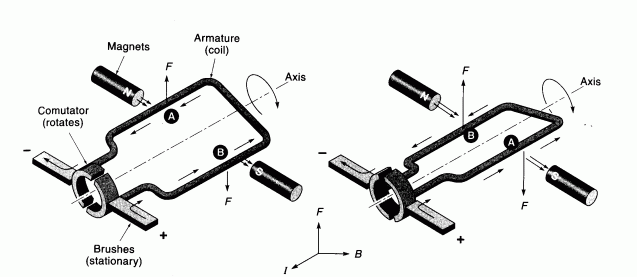
\includegraphics[height=7cm]{figures/dc_conducting_wire.png}
	\caption{A single current conductor in a static magnetic field \cite{dc_motor_2}}
	\label{dc_conducting_wire}
\end{figure}
At some point the magnetic fields would align resulting in a zero torque. In brushed DC motors this switching mechanism is done by the so called commutator part. Figure \ref{dc_conducting_wire} represent a single wire with a commutator. The commutator is a simple mechanical switch that changes the polarity of the voltage put on the wire by touching the brushes in order to make the current flow in such a direction that maintains the direction of the generated torque, therefore the armature continue rotating. A single wire would provide a fluctuating torque during the operation since the angle between the coil and static magnetic flux is changing. For a more smooth operation of the rotor, several separate wire loops have to be used shifted from each other and switched one after the other. This can be realized by applying more pairs of commutators which enables to connect always that coil loop with power source that does not align with the permanent magnetic field, thus can produce maximum torque. In practical motors the rotating part is called armature and standing part is called stator. The stator can be a permanent magnetic pole in case of small DC motors, while in larger motors an electromagnet is used which is also powered by the same DC source in serial or parallel connection. In my case, the motor has a permanent magnetic stator.
According to Faraday's law of electromagnetic induction, a rotating loop of coil will produce an electromotive force called EMF. The case of the rotating armature loop is the same, thus in this case it produces an adverse electromotive force which is called back EMF that tends to decrease cause of the accelerating effect, i.e. the applied input voltage. As a result, the back EMF will decrease the armature current by a remarkable amount, thus the motor torque as well. \cite{dc_motor_1} \cite{dc_motor_2}

The electrical equivalent circuit of the armature and the free-body diagram of the rotor can be modeled as follows.
\begin{figure}[htb!]
	\centering
	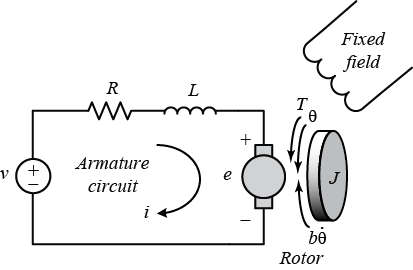
\includegraphics[height=7cm]{figures/dc_motor_model.png}
	\caption{DC motor electrical and mechanical model \cite{dc_motor_3}}
	\label{dc_motor_model}
\end{figure}

The motor is supplied with $V$ voltage as an input, while the output is the rotational speed of the rotor and shaft (rigid connection). In the mechanical model the load torque ($T_L$) and also dissipation energy is considered as being proportional with the angular speed. The motor torque is generally proportional to the armature current and the strength of the magnetic field, but in this model the magnetic field is assumed to be constant, thus the motor torque depends on the armature current ($i$) only. The back emf ($e$) is proportional to the angular velocity of the shaft. If SI units are used then the constants of the torque and the emf are equal, thus the same ($K$) constant can be used for the following equations:\cite{dc_motor_3}\cite{dc_motor_4}
\begin{equation}
T = K i
\end{equation}
\begin{equation}
e = K \dot \theta
\end{equation}		

Based on the model in Figure \ref{dc_motor_model} the following equations can be derived by means of the Newtons's 2nd Law and Kirchoff's voltage law.
\begin{equation}
J \ddot \theta + b \dot \theta = K i - T_L
\label{dc_eq_1}
\end{equation}
\begin{equation}
L \frac{di}{dt} + R i = V - K \dot \theta
\label{dc_eq_2}
\end{equation}
The system can be described by a system of linear differential equations with respect to armature current and rotor angular velocity. A given system can be defined by 5 parameters, i.e. armature resitance (R), armature inductance (L), motor constant (K), damping constant (b) and motor inertia (J).
\subsubsection{Step response analysis of the motors}
The motors speeds can be changed via PWM and with the help of the rotary encoders the response function to any voltage value could be measured. It is more convenient to treat the PWM signal's duty cycle as the control input although voltage level is applied to the armature of the motor. The PWM signal's duty cycle is determined in the code by a floating point number between zero and one. Firstly, let the pwm value be regarded as an input and the wheel speed as an output assuming that the transfer function of the gearbox and power electronic module are proportional type, thus it can be handled together with the motor as a plant element. 
The motors gave a quite similar responses with respect to time constant and amplitude and also the nominal value (107RPM at 12V no load case) was obtained with small deviations. 

\begin{figure}[htb!]
	\centering
	\minipage{0.48\textwidth}
	\centering
	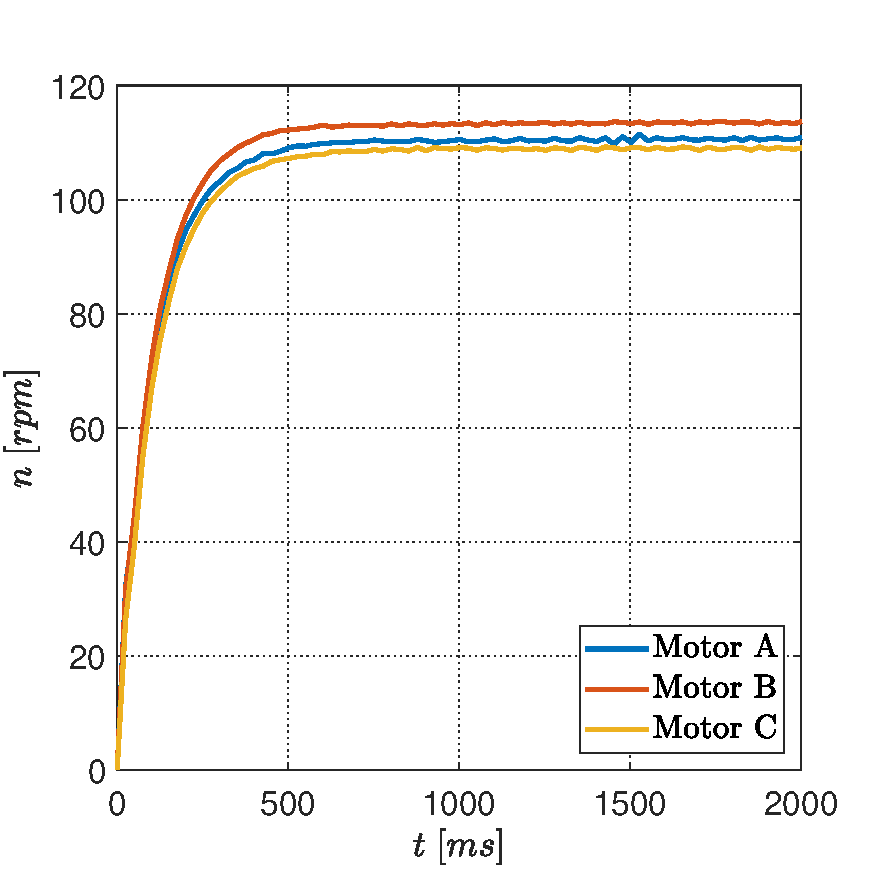
\includegraphics[width=0.9\textwidth]{figures/directed_speed_pwm_100}
	\caption{PWM=100\% step response of the motors}
	\label{directed_speed_pwm_100}
	\endminipage\hfill
	\minipage{0.48\textwidth}
	\centering
	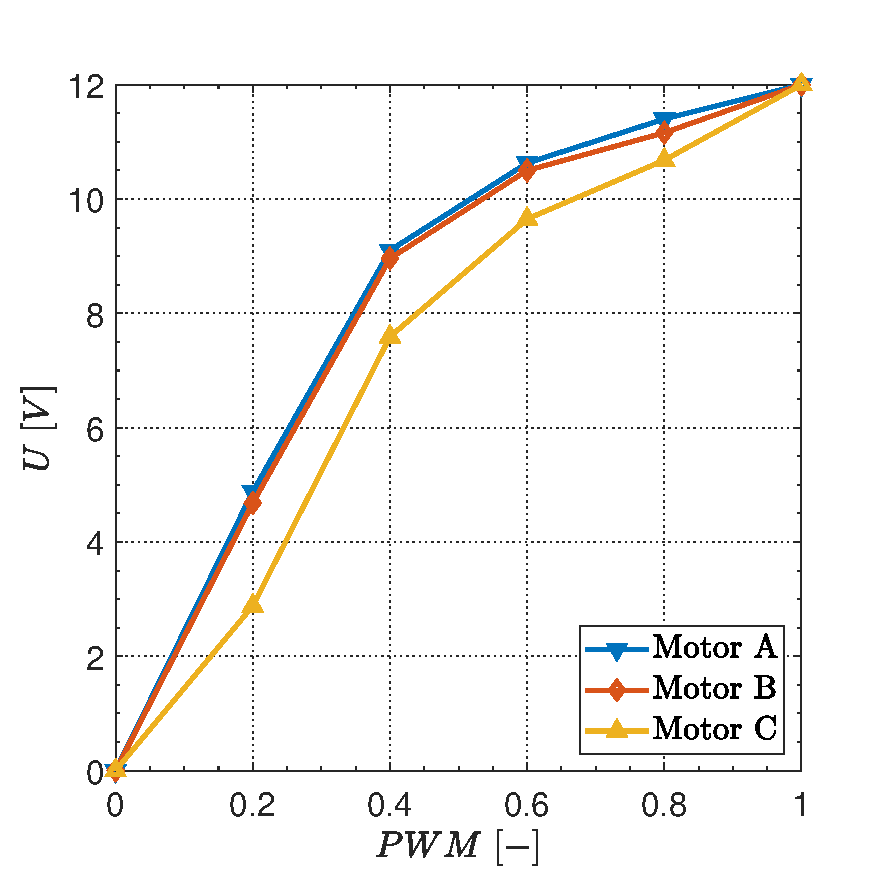
\includegraphics[width=0.9\textwidth]{figures/pwm_u}
	\caption{Nonlinearity of the PWM-U relation}
	\label{pwm_characteristic}
	\endminipage\hfill
\end{figure}
\begin{figure}[htb!]
	\centering
	\minipage{0.48\textwidth}
	\centering
	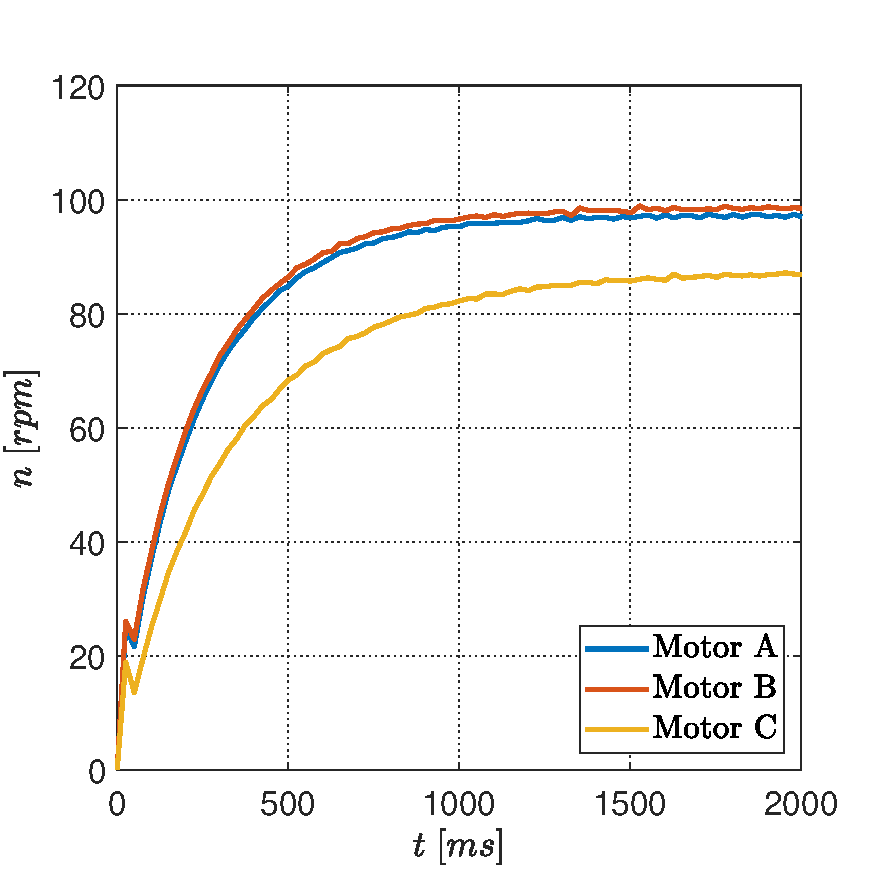
\includegraphics[width=0.9\textwidth]{figures/directed_speed_pwm_60}
	\caption{PWM=60\% step response of the motors}
	\endminipage\hfill
	\minipage{0.48\textwidth}
	\centering
	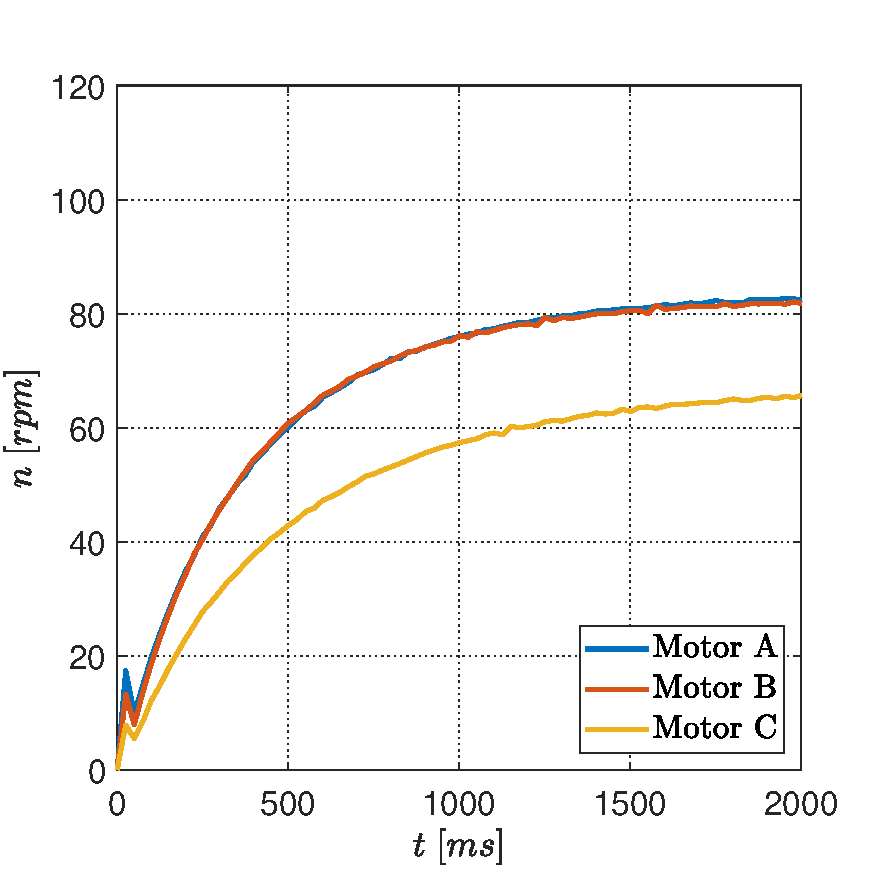
\includegraphics[width=0.9\textwidth]{figures/directed_speed_pwm_40}
	\caption{PWM=40\% step response of the motors}
	\label{mecanum}
	\endminipage\hfill
\end{figure}
Unfortunately, the problems were captured when the duty cycle of the pwm signal was decreased, i.e. the pwm value in the Arduino code. The prior guess that the pwm value provided in the MCU code will be proportional to the motor speeds was proven to be wrong. Furthermore one of the L298N module was functioning with a different characteristic as the other driver as it provided different voltage values for the same pwm signal which resulted that the Motor C was spinning remarkably slower. It is also clearly visible that the system is nonlinear as neither for the Motor A and B the same dynamics with respect to rise time were obtained, thus even the time constants were not similar.
It is obvious that without proper control of the wheels it is hard to achieve smooth and accurate movements which is one of our main design criteria. As a first approximation, it is worth neglecting the mentioned issues and handle the system as it would be completely linear. This is defenietly not true but a good approcimation. Further problems could occur at low voltages, i.e. pwm values less than 0.2 where the system probably become extremely nonlinear as the motor will not move at such small voltages where the generated motor torque is not strong enough to overcome sticking friction. Though the linear viscous friction is included in the model presented in the next chapter as it is easy to calculate with. A possible practical solution is to have the motor banned to work in the problematic regions. 
\newpage
\subsubsection{Controller design using blackbox model}
Considering the system as being linear in theory based on the response function corresponding to any pwm signal, a controller can be designed for the whole range for each wheel separately. In order to do this, a black box model has to constructed. In case of a DC motor it is a typical procedure to handle the system as a first order one. \cite{dc_motor_3} 
Applying the Laplace transform on Eq.\ref{dc_eq_1} and \ref{dc_eq_2}, then rearranging the transformed equations the transfer function of the system is as follows:
\begin{equation}
G(s) = \frac{\dot \theta (s)}{V(s)} = \frac{K}{(Js+b)(Ls+R)+K^2}.
\end{equation} 
Beside the fact that a second-order model can be derived, the step response of dc motors usually looks like that of a first-order system. After inspecting the actual step response of the given motors, it looks as a good approximation. It can be explained by the fact that the motor is an overdamped second-order system, in other words it has two negative poles (roots of the denominator of the transfer function). Such a system is stable and has two time constants. In case of DC motors, the time constant of the mechanical dynamics is much higher compared to the time constant of the electrodynamics, thus the slower mechanical dynamics dominates the overall time response. 
A first order system can be expressed as it follows:
\begin{equation}
P(s) = \frac{\dot{\theta}(s)}{DC(s)}= \frac{k}{1+\tau s},
\end{equation}
where
\begin{itemize}
	\item $DC(s)$ - Laplace tranform of the duty cycle signal, $P(s)$ - plant tranfer function
	\item $\tau$ - time constant which equals the time it takes the system to reach the 63.2\% of steady-state step response of a unit step, more generally it represents the time scale of the system dynamics,
	\item $k$ - gain, the ratio of the magnitude of the steady-state step response to the magnitude of the step input.
\end{itemize}
Based on the measurments shown in Figure \ref{directed_speed_pwm_100} the following values were calculated providing a really good agreement.
\begin{table}[h]
	\centering
	\label{first_order_model_table}
	\begin{tabular}{cccc}
		\hline
		& A  		& B  		& C   		\\ \hline
		$k$ {[}rpm{]} 		& 111.05 	& 113.39 	& 109.07 	\\
		$\tau$ {[}ms{]}       & 100.70 	& 99.88 	& 107.03   	\\ \hline
	\end{tabular}
	\caption{First-order model parameter estimations}
\end{table}
A common choice for such a system is a PI controller.\cite{dc_motor_3} The plant block is overall model of the power electronic module, the motor armature, rotary encoders and the signal processing on the MCU. 
\begin{figure}[htb!]
	\centering
	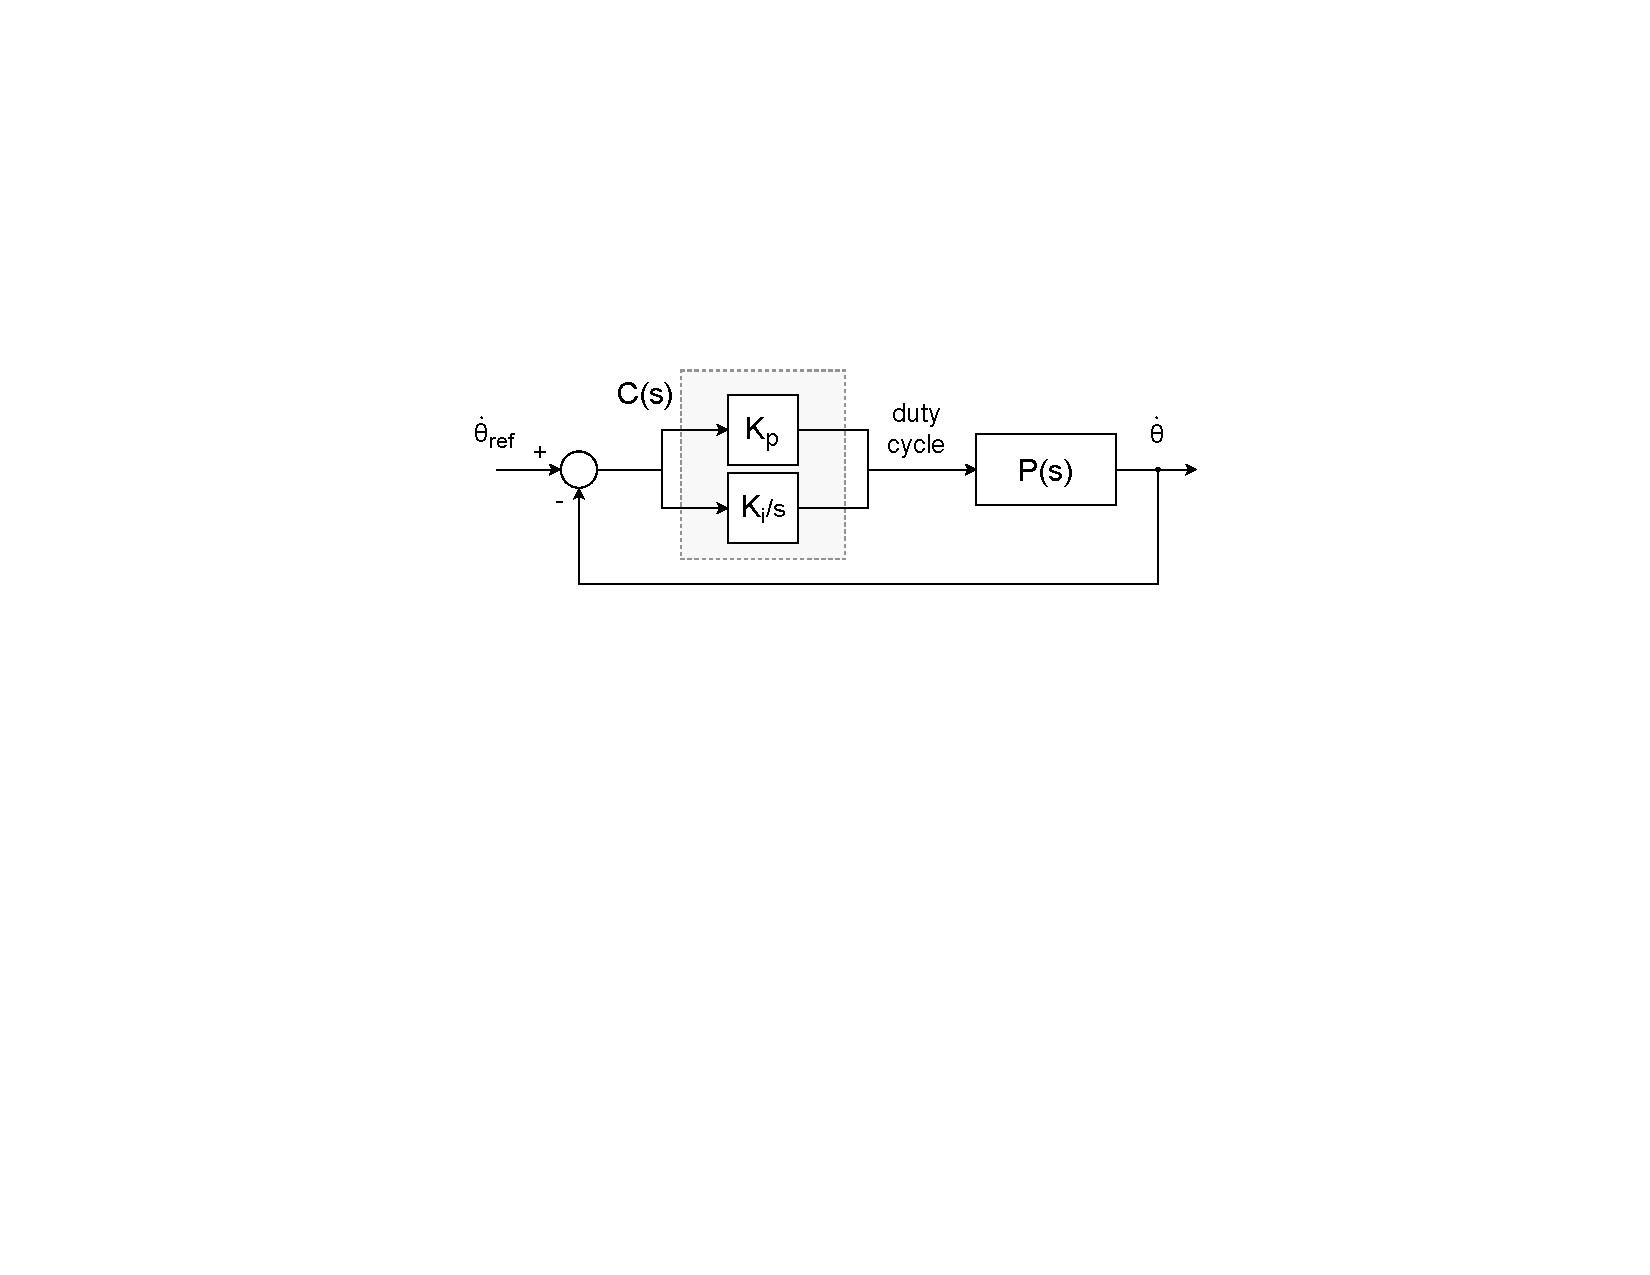
\includegraphics[width=0.7\textwidth]{figures/control_block_diagram}
	\caption{Model of the closed (feedback controlled) system}
	\label{dc_motor_closed_system}
\end{figure}
The transfer function of the controller PI (proportional-integrating) is as follows:
\begin{equation}
C(s) = K_p + \frac{K_i}{s}.
\end{equation}
The transfer function of the (negative feedback) closed-loop:
\begin{equation}
T(s) = \frac{C(s)P(s)}{1+C(s)P(s)}=\frac{A (K_i+K_p s)}{A K_i+A K_p s+s^2 \tau +s}
\label{eq_transfer_function}
\end{equation}
The closed-loop system is almost a second-order one except for the presence of the zero (possible root in the denominator), thus it does not match with the canonical form exactly:
\begin{equation}
G(s) = \frac{{k \omega_n}^2}{s^2 + 2 \zeta \omega_n s +{\omega_n}^2}
\label{eq_transfer_function_canonical}
\end{equation}
where
\begin{itemize}
	\item $k$ - gain is the ratio of the magnitude of the steady-state step response to the magnitude of the step input,
	\item $\zeta$ - The damping ratio is a dimensionless quantity characterizing the rate at which an oscillation in the system's response 		decays due to effects such as viscous friction or electrical resistance,
	\item $\omega_n$ - The natural frequency is the angular frequency that the system will oscillate at when there is no damping. \cite{dc_motor_3}
\end{itemize}

The original system is overdamped but the addition of a proportional controller can make it underdamped as it has similar behaviour like a "virtual spring". For such special case several design equations are available if the parameters in the canonical form are known. The presence of the zero in closed-loop transfer function can be a cause of errors. However, as a first guess it can provide a good approximation for starting value for the controller if the presence of zero is not considered and the system is treated as if it was an underdamped second-order system.
It is important to mention, that the closed-loop system would have a canonical form if only proportional type controller was used.

The canonical second-order transfer function has two poles at:
\begin{equation}
s_p = -\zeta \omega_n \pm j \omega_n \sqrt{1-{\zeta}^2} = -\sigma \pm j\omega_d.
\label{eq_poles}
\end{equation}
If $\zeta<1$, then the system is underdamped, the two poles are both complex-valued with negative real parts ($\sigma$<0). The system is asymptotically stable and oscillating with the damped natural frequency $\omega_d = \omega_n \sqrt{1-{\zeta}^2}$. Based on the value of damping the system can marginally stable and unstable, but those are not the cases which are have to be examined now.

Combining the denumerators of equation (\ref{eq_transfer_function}) and (\ref{eq_transfer_function_canonical}) the following expressions can be obtained:
\begin{equation}
{\omega_n}^2 = \frac{A K_i}{\tau},
\end{equation}
\begin{equation}
2\omega_n\zeta  = \frac{1+A K_p}{\tau}.
\end{equation}
Additionally using the equation \ref{eq_poles}, the relation between the poles of the closed loop and the controller parameters can be derived:
\begin{equation}
%{\omega_d}^2 = \frac{A K_i (1-\zeta^2)}{\tau},
\sigma^2 + {\omega_d}^2 = \frac{A K_i}{\tau},
\label{eq_pi_from_poles_1}
\end{equation}
\begin{equation}
\sigma = \frac{1+A K_p}{2\tau}.
\label{eq_pi_from_poles_2}
\end{equation}

Figure \ref{second_order_underdamped_response} represents the step response of a canonical second order system and several properties are denoted to characterize itself.
\begin{figure}[htb!]
	\centering
	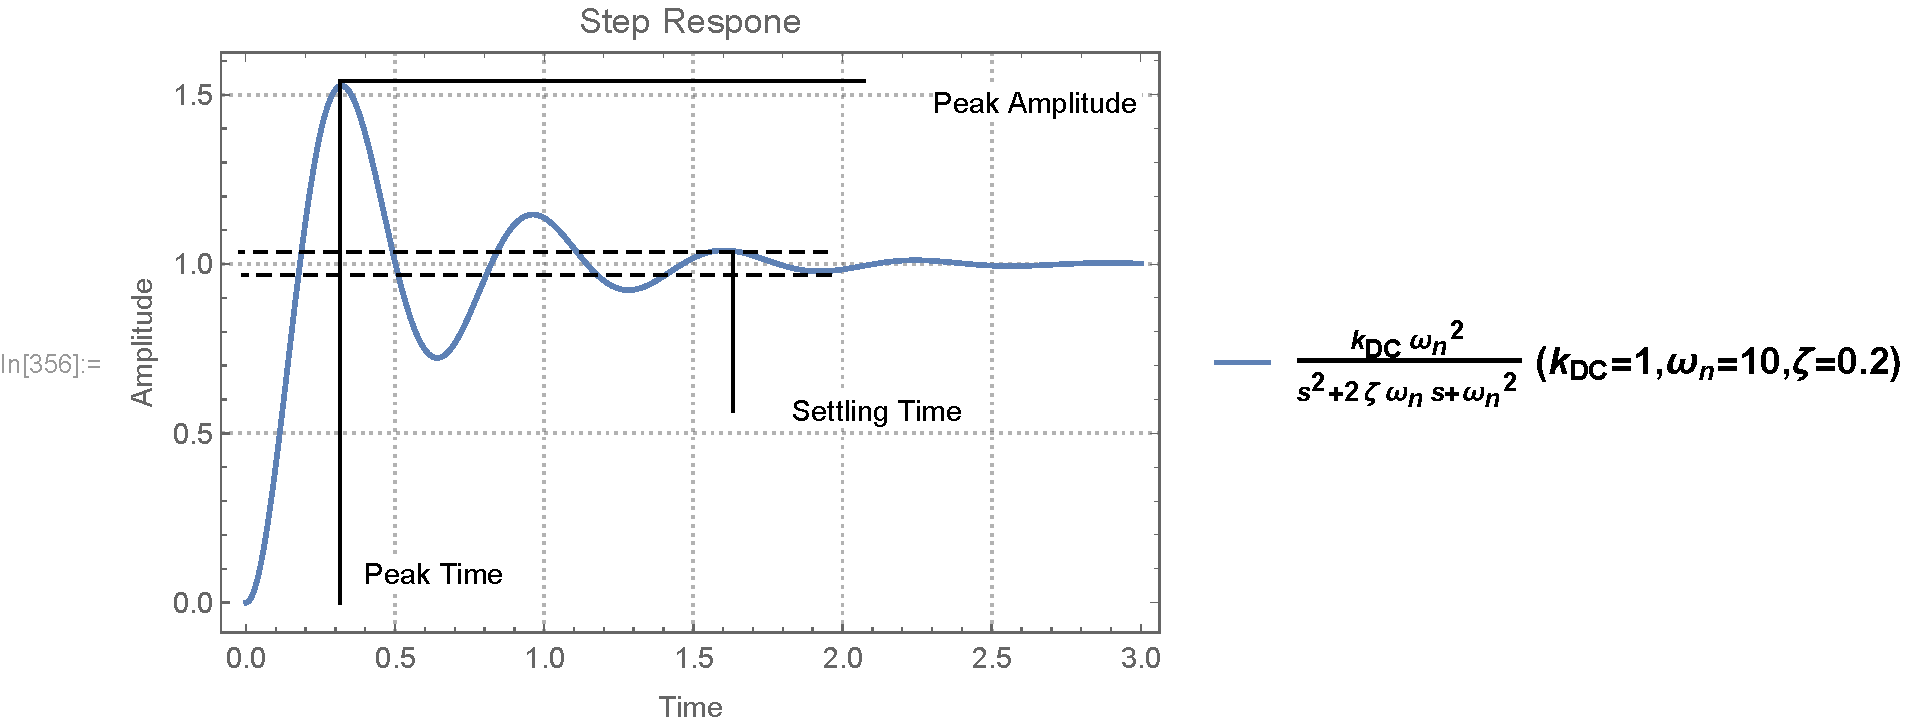
\includegraphics[height=7cm]{figures/step_response_of_2nd_order_system_1}
	\caption{Step response characteristics of $v(t)=\frac{k ~ {\omega_n}^2}{s^2+2 \zeta \omega_n s + {\omega_n}^2}$ where $k=1$, ${\omega_n}=10$, $\zeta=0.2$.}
	\label{second_order_underdamped_response}
\end{figure}
\begin{itemize}
	\item Settling Time is the time that the system needs to have an output with a smaller deviation from the steady-state in terms of a given percentage. In case of second-order canonical system the following formula provides a good approximation: \cite{dc_motor_3}
	\begin{equation}
	T_s = -\frac{ln(tolerance)}{\zeta \omega_n} = -\frac{ln(tolerance)}{\sigma}
	\label{eq_settling_time}
	\end{equation}
	\item Percent Overshoot characterize the output in terms of the ratio of maximum peak and the steady-state value expressed as a percentage. \cite{dc_motor_3}
	\begin{equation}
	Mp = e^{\frac{-\zeta \pi}{\sqrt{1-\zeta^2}}}
	\label{eq_overshoot}
	\end{equation}
	The corresponding peak time is as follows: \cite{dc_motor_3}
	\begin{equation}
	T_p = \frac{\pi}{\omega_d}
	\label{eq_overshoot_time}
	\end{equation}
\end{itemize}
Ideally closed-loop respond with low settling time and overshoot is wanted. Limits can be defined in arbitrary way that suits are demands with respect to the former properties. Based on equations \ref{eq_settling_time}, \ref{eq_overshoot} and \ref{eq_overshoot_time} further limits can be derived for $\zeta$ and $\omega_d$.
\begin{itemize}
	\item 1 \% settling time:
	\begin{equation}
	T_s = -\frac{ln(0.01)}{\sigma} = \frac{4.605}{\sigma} < l_{T_s},
	\end{equation}
	\begin{equation}
	\sigma > \frac{4.605}{l_{T_s}}.
	\end{equation}
	
	\item peak time:
	\begin{equation}
	T_p = \frac{\pi}{\omega_d} < l_{T_s},
	\end{equation}
	\begin{equation}
	\omega_d > \frac{\pi}{l_{T_p}}.
	\end{equation}
	
	\item maximum percent overshoot:
	\begin{equation}
	Mp = e^{\frac{-\zeta \pi}{\sqrt{1-\zeta^2}}}  < l_{M_p},
	\end{equation}
	\begin{equation}
	\zeta > \sqrt{\frac{ln^2(l_{M_p})}{\pi^2+ln^2(l_{M_p})}}.
	\end{equation}
\end{itemize}
where $l_{T_s}$, $l_{T_p}$ and $l_{M_p}$ are the limits respectively.
Considering the provided limits, some guidelines for seeking suitable poles can be obtained which probably result desired system dynamics. Rearranging the equations \ref{eq_pi_from_poles_1} and \ref{eq_pi_from_poles_2}, the controller gain estimations can be calculated:
\begin{equation}
K_p = \frac{2 \sigma \tau - 1}{A},
\end{equation}
\begin{equation}
K_i = \frac{\tau(\sigma^2 + {\omega_d}^2)}{A}.
\end{equation}
As it was mentioned before, choosing the poles based on the above limits can not guarantee acceptable system behaviour as our system is not a canonical second-order, on the top of that the plan model is also simplified to a first order and not even any nonlinearity is considered.
\begin{figure}[htb!]
	\centering
	\minipage{0.45\textwidth}
	\centering
	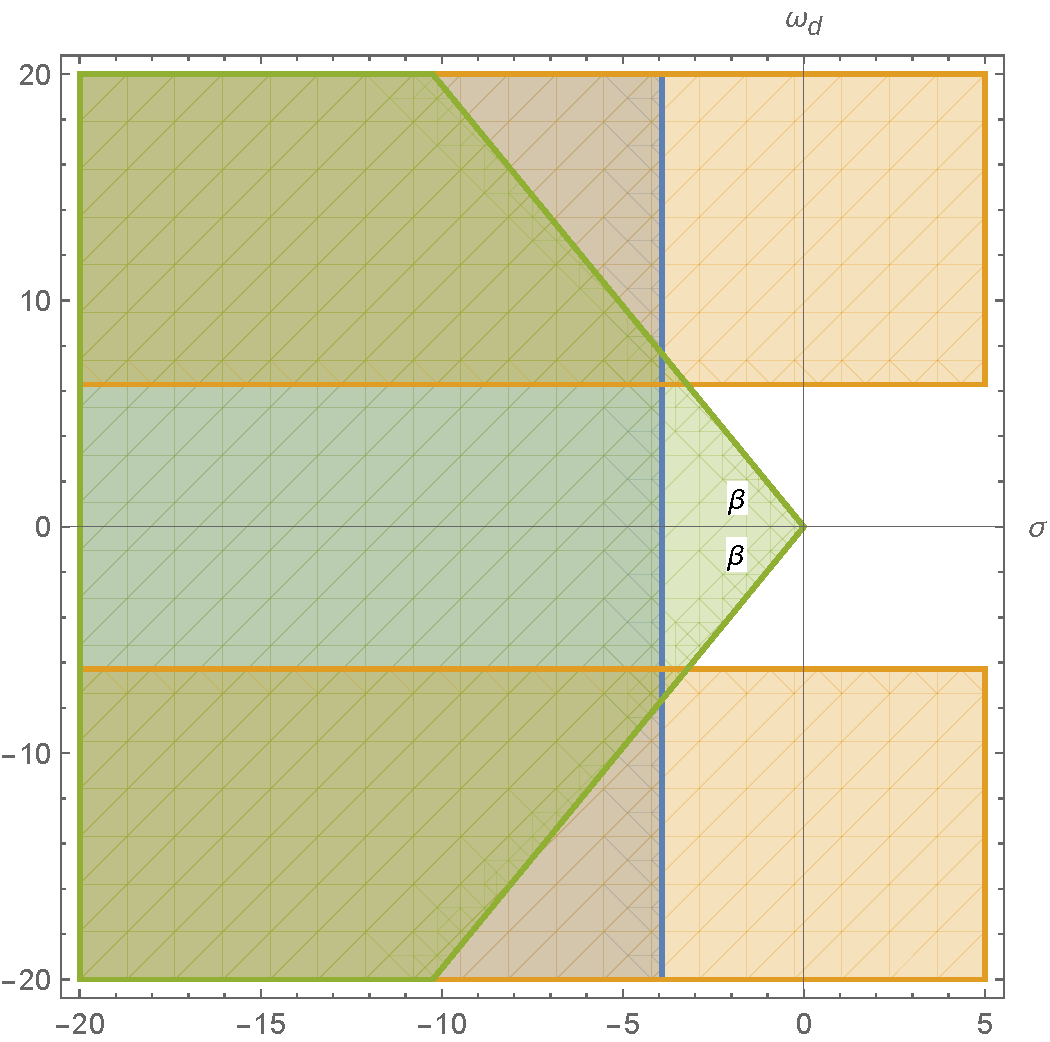
\includegraphics[width=\textwidth]{figures/possible_poles}
	\caption{Pole parameter field considering the limits: settling time limit (blue), peak time limit (orange) and overshoot limit (green)}
	\label{possible_poles}
	\endminipage\hfill
	\minipage{0.45\textwidth}
	\centering
	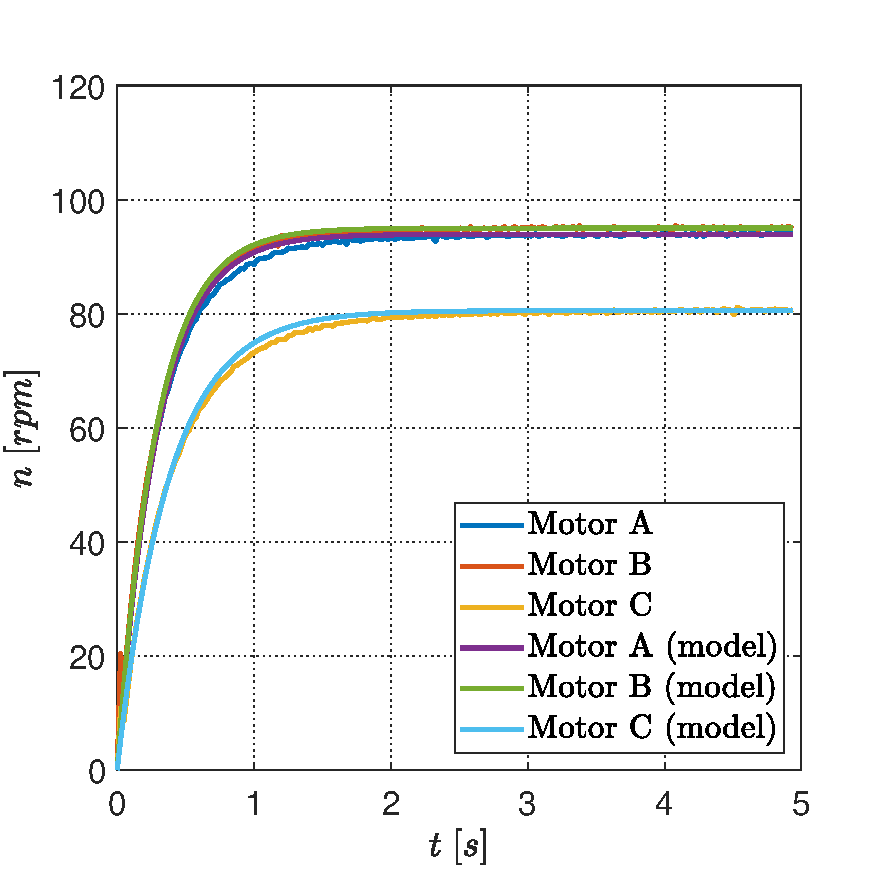
\includegraphics[width=\textwidth]{figures/directed_speed_pwm_50_fitted}
	\caption{Black box model at 0.5 PWM value}
	\label{fitted_model}
	\endminipage\hfill
\end{figure}

Figure \ref{possible_poles} shows the possible real and imaginary value pairs which satisfies the requirements. The real part of pole is $\sigma$, the imaginary part is $\omega_d$ and the angle $beta$ can calculated by means of $\zeta = cos(\beta)$. \\[2mm]
\noindent Let us have the following requirements:
\begin{itemize}
	\item Settling time for 1$\%$: 2[s]
	\item Peak time: 1[s]
	\item Max peak amplutude: 10\%
\end{itemize}
\noindent and let us use measurments corresponding to pwm value of 0.5. After fitting the first order balck box model the following values were obtained.
\begin{table}[h]
	\centering
	\label{first_order_model_table_50}
	\begin{tabular}{cccc}
		\hline
		& A  		& B  		& C   		\\ \hline
		$\tau$ {[}s{]} 		& 0.2949 	& 0.2880 	& 0.3767 	 \\
		$k$ {[}rpm{]}       & 93.8978 	& 94.9998 	& 80.5325   	\\ \hline
	\end{tabular}
	\caption{First-order model parameter estimations}
\end{table}
Considering the given requirements, as a first approximation placing the poles of the system to $\sigma = 5$ and $\omega_d = \pi$ point can be good.
In this case, the $K_p = 0.021$ and $K_i = 0.11$ are obtained.
\begin{figure}[htb!]
	\centering
	\minipage{0.45\textwidth}
	\centering
	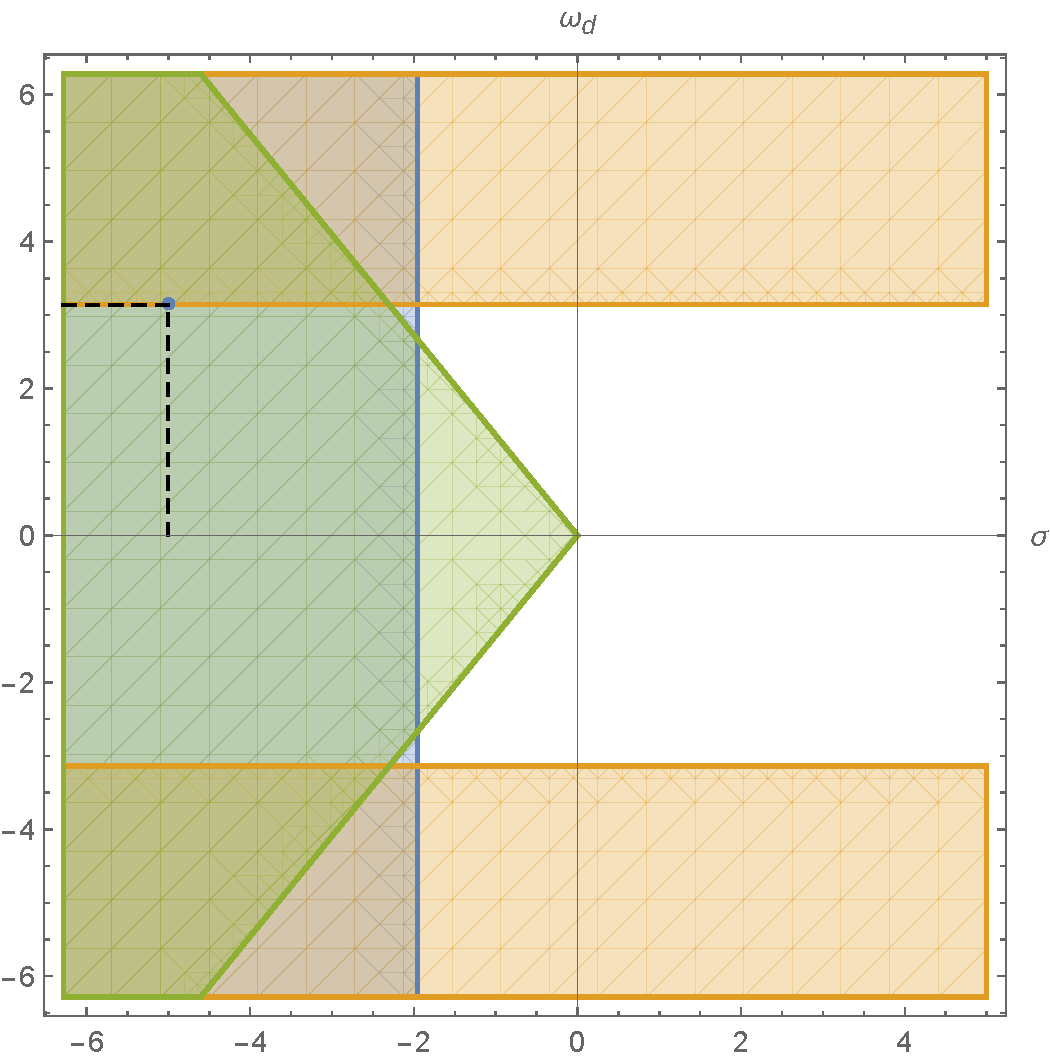
\includegraphics[width=\textwidth]{figures/polemap_at_50}
	\caption{Possible poles that suits the requirements, the pole combination represented by the point is chosen in an arbitrary way considering the limits}
	\label{polemap_at_50}
	\endminipage\hfill
	\minipage{0.45\textwidth}
	\centering
	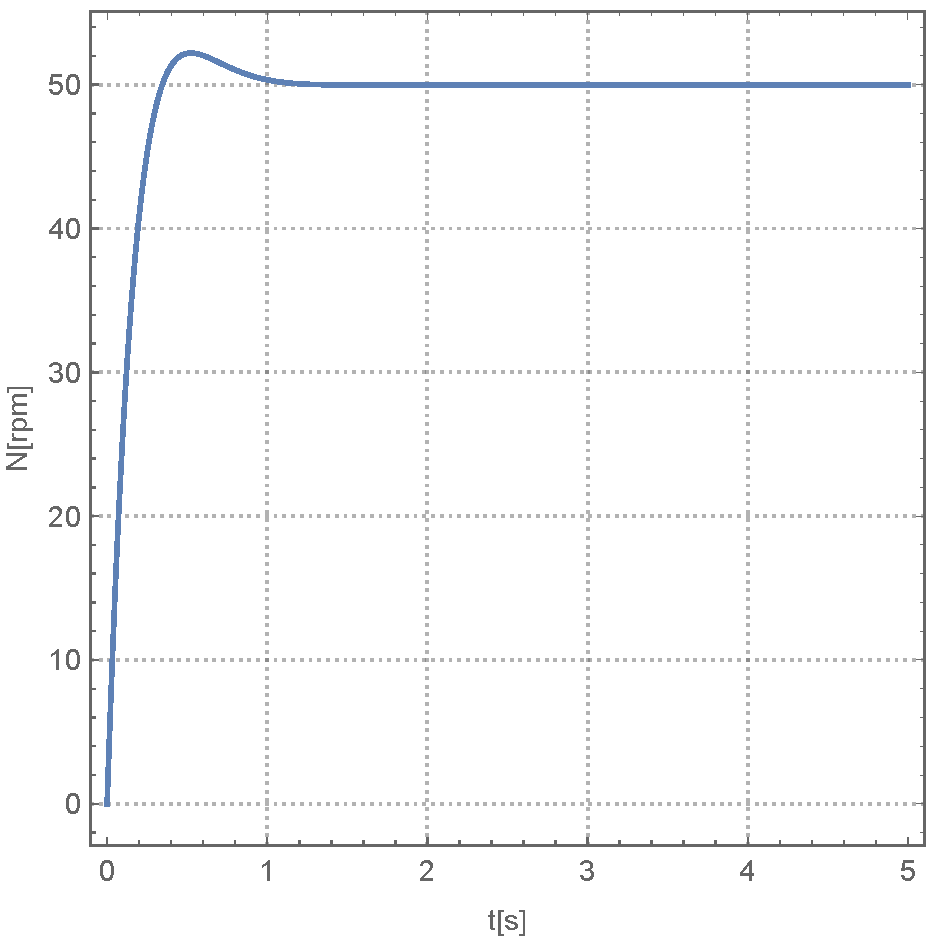
\includegraphics[width=\textwidth]{figures/expected_50}
	\caption{Expected response}
	\label{expected_response_50}
	\endminipage\hfill
\end{figure}

The system responses are shown in Figure \ref{obtained_response_50} and \ref{obtained_response_100}. In case of target speed of 100 rpm, the controller makes a really bad performance with so high oscillations. The oscillations vanishes if the integral type controller gain is set to zero, but the final value will be uncertain. After some trial and error for seeking a better integral gain an acceptable combination were found. The corresponding system responses are presented in Figure  \ref{obtained_response_50_good} and \ref{obtained_response_100_good}. The only prelimanary criteria which was not fulfilled is the max peak amplitude in case of $50\%$ PWM, when it was about $15\%$ instead of $10\%$. However, better peak and settling times were obtained.
\newpage
\begin{figure}[htb!]
	\centering
	\minipage{0.45\textwidth}
	\centering
	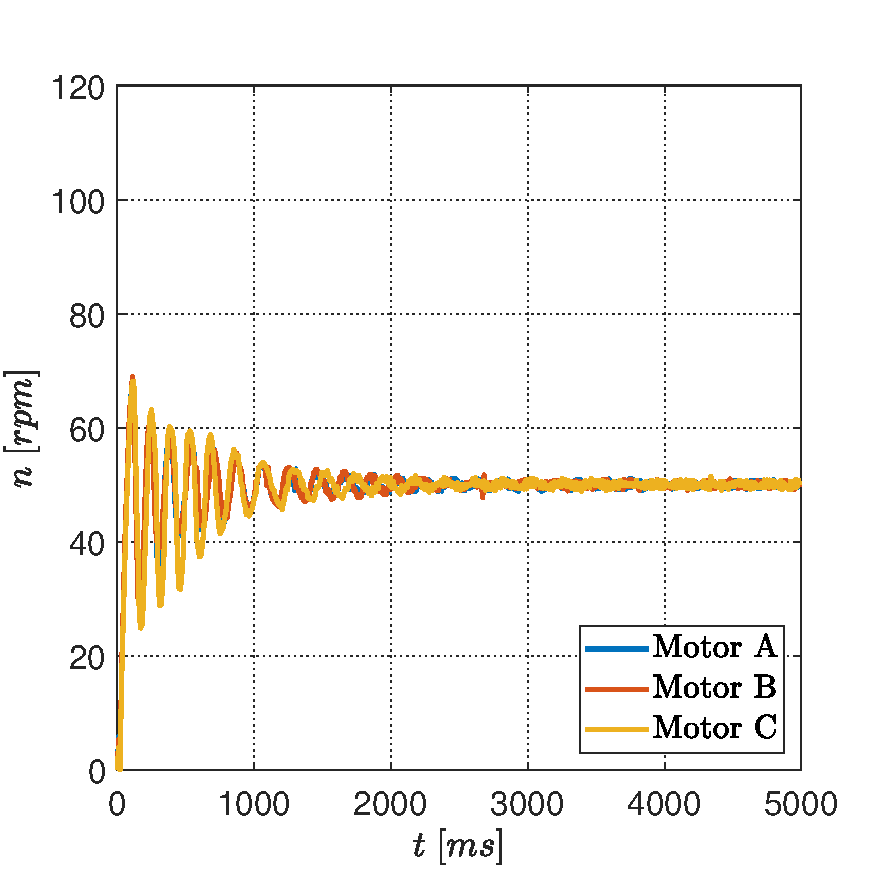
\includegraphics[height=7.5cm]{figures/controlled_50_p_02_i_11}
	\caption{Obtained response at target velocity 50 [rpm]}
	\label{obtained_response_50}
	\endminipage\hfill
	\minipage{0.45\textwidth}
	\centering
	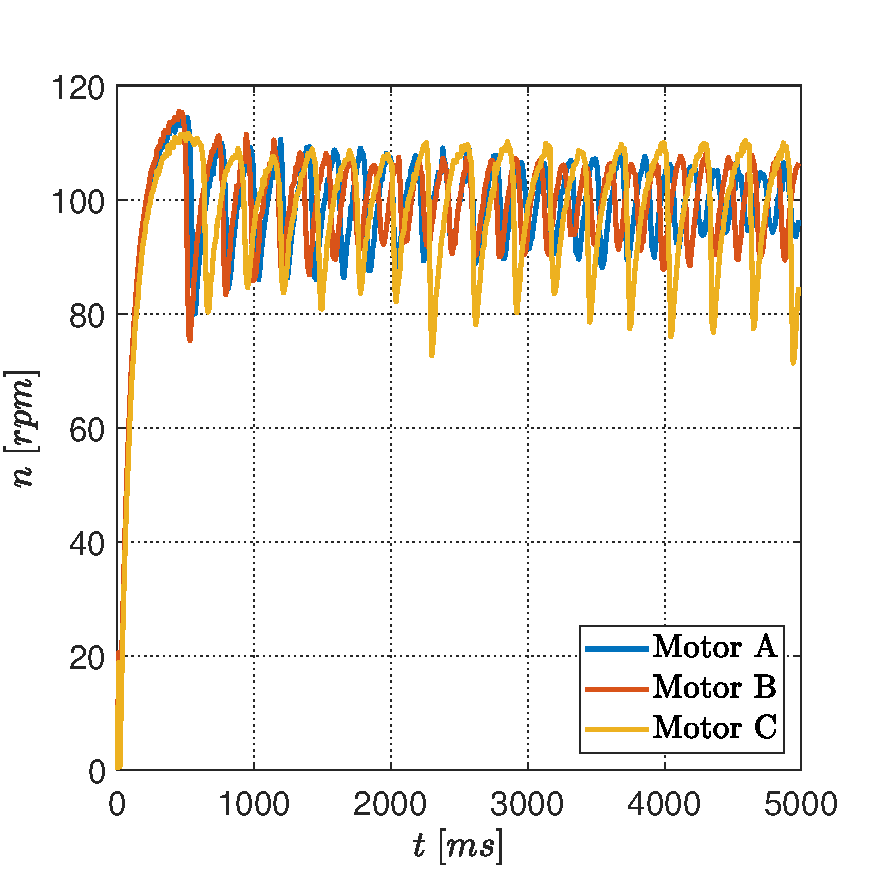
\includegraphics[height=7.5cm]{figures/controlled_100_p_02_i_11}
	\caption{Obtained response at target velocity 100 [rpm]}
	\label{obtained_response_100}
	\endminipage\hfill
\end{figure}
\begin{figure}[htb!]
	\centering
	\minipage{0.45\textwidth}
	\centering
	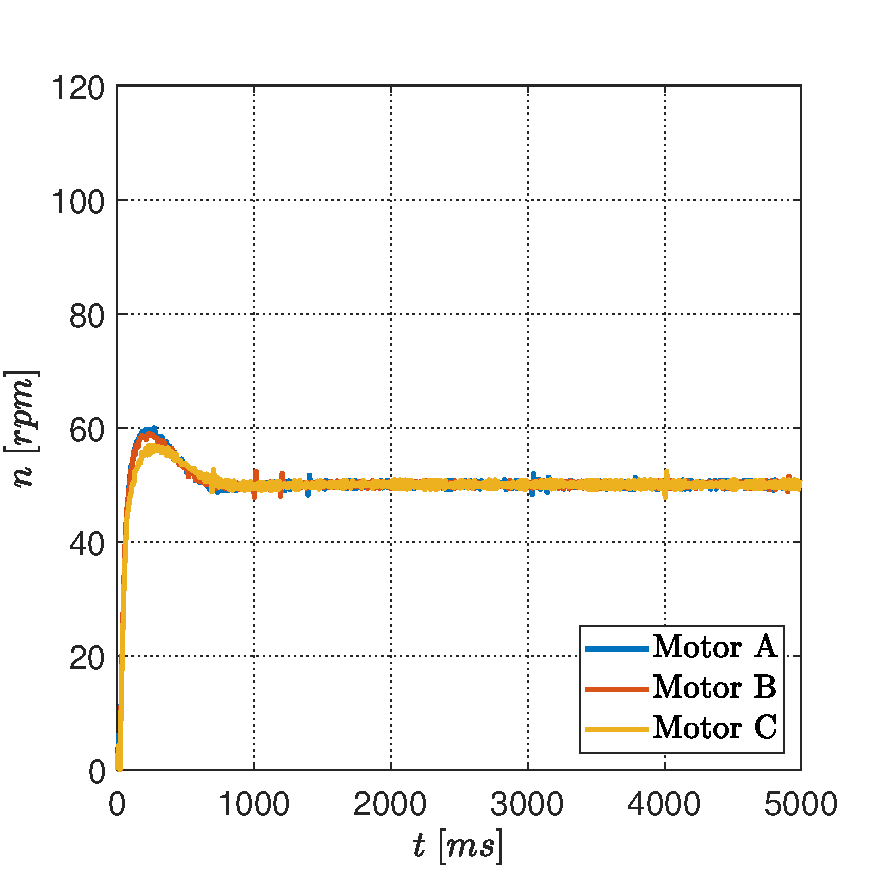
\includegraphics[height=8cm]{figures/controlled_50_p_02_i_002}
	\caption{Obtained response at target velocity 50 [rpm]}
	\label{obtained_response_50_good}
	\endminipage\hfill
	\minipage{0.45\textwidth}
	\centering
	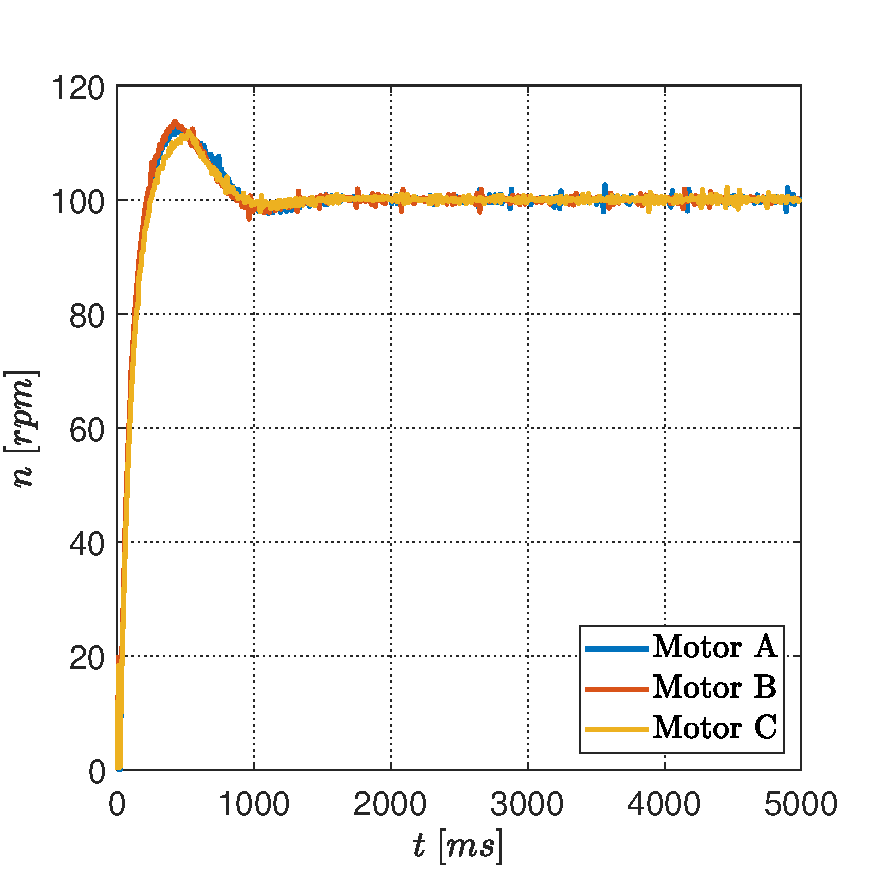
\includegraphics[height=8cm]{figures/controlled_100_p_02_i_002}
	\caption{Obtained response at target velocity 100 [rpm]}
	\label{obtained_response_100_good}
	\endminipage\hfill
\end{figure}
\newpage

\newpage
\section{Motion Analysis of The Robot}
\subsection{Kinematics of three-wheeled omnidirectional robot}
\subsubsection{Basic relationships}
Let us define the global frame as [X,Y] coordinate system which represents the environment. The location and the orientation of the robot can be described with (X,Y,$\alpha$) or (X,Y,$\varphi$) vector, while the kinematic state is that of time-derivative, i.e. ($\dot X, \dot Y, \dot \alpha$) or ($\dot X, \dot Y, \dot \varphi$). Eventually, we are usually interested in the kinematics from global frame point of view, but from the design and user point of view it is more convenient to start writing the equations in the local frame of the robot and then transform the kinematics to the global frame if that is needed. Let us denote the local frame as $(x,y)$ which center is the center of gravity of the robot. The robot velocity as $v$ when that of components in the local frame are $(v_x,v_y) = (- v sin \gamma , v cos \gamma )$.

\begin{figure}[htb!]
	\centering
	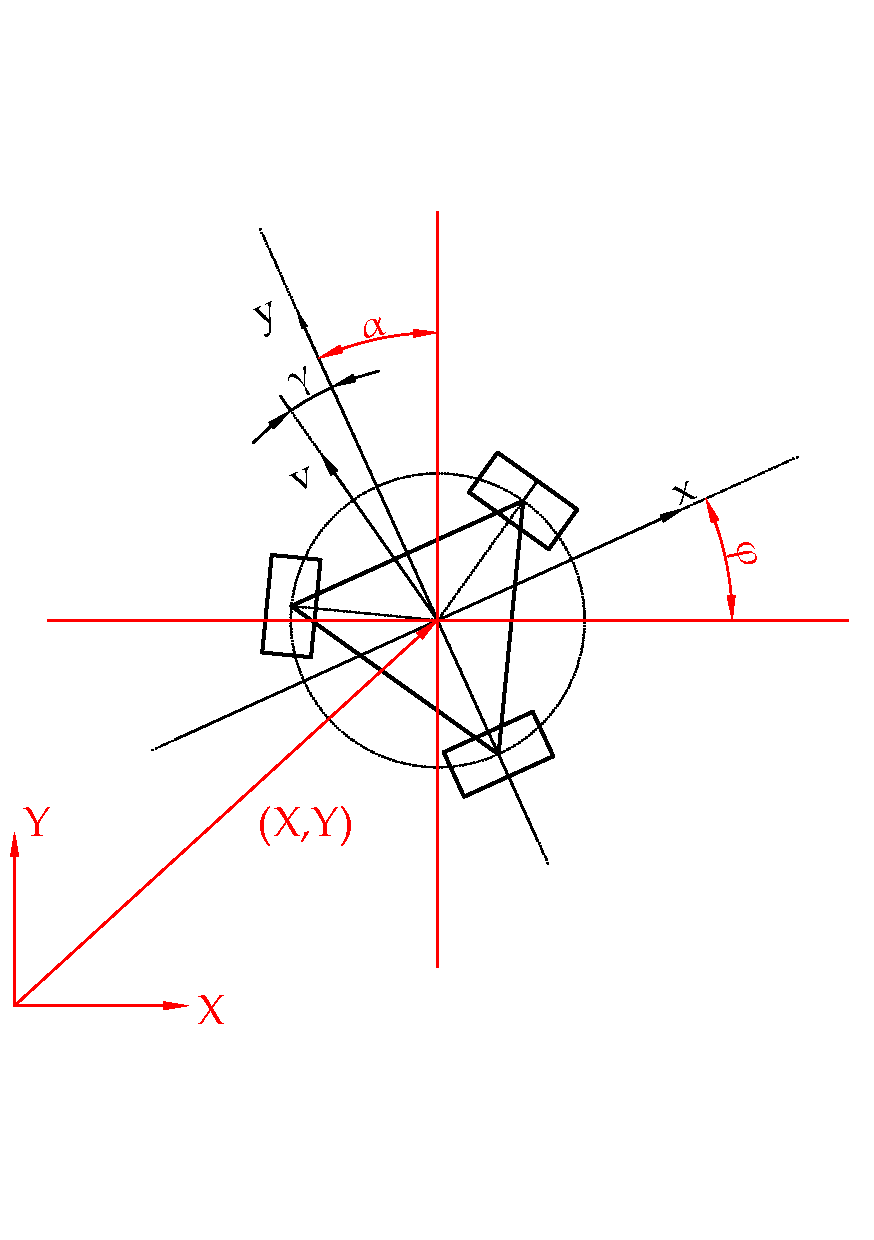
\includegraphics[width=7cm]{figures/global_local_frame}
	\caption{Global and local frames of the robot}
	\label{global_local_frame}
\end{figure}
The overall kinematic state of the case is a straightforward resultant of the wheel kinematic states. The velocity of wheels can have two type of components:
\begin{itemize}
	\item Translational velocity which actually equals with translational speed of the case because of the kinematic constraint. Additionally, it can be divided into two further parts:
		\begin{itemize}
			\item Its own velocity which can be called as pure translational wheel speed. It is proportional with the angular velocity of the wheel: $v_{wheel,t} \sim r \omega_i$, where r is the wheel radius and $\omega$ is the angular velocity.
			\item The rolling velocity $v_{roller}$ which is induced by the other wheels and realized by the free rollers. Its direction is determined by the construction of rollers, generally and also in this case let it assume to be 90$^{\circ}$.
		\end{itemize}
	\item Rotational velocity component which comes from the spinning of the whole robot case about its center of gravity which can be supposed to be in the geometrical center of the common wheel circle, therefore it can be formulated as $v_{wheel,r}  = R \dot \alpha$. This component is always the same for all wheels.
\end{itemize}
The resultant translational wheel velocity can be calculated as:
\begin{equation}
v^i = {v_{wheel,t}}^i + {v_{wheel,r}} = r \omega_i
\end{equation}
where $i$ is the index of the wheels and i=1,2,3 in case of a thee-wheeled omnidirectional robot.
\begin{figure}[htb!]
	\centering
	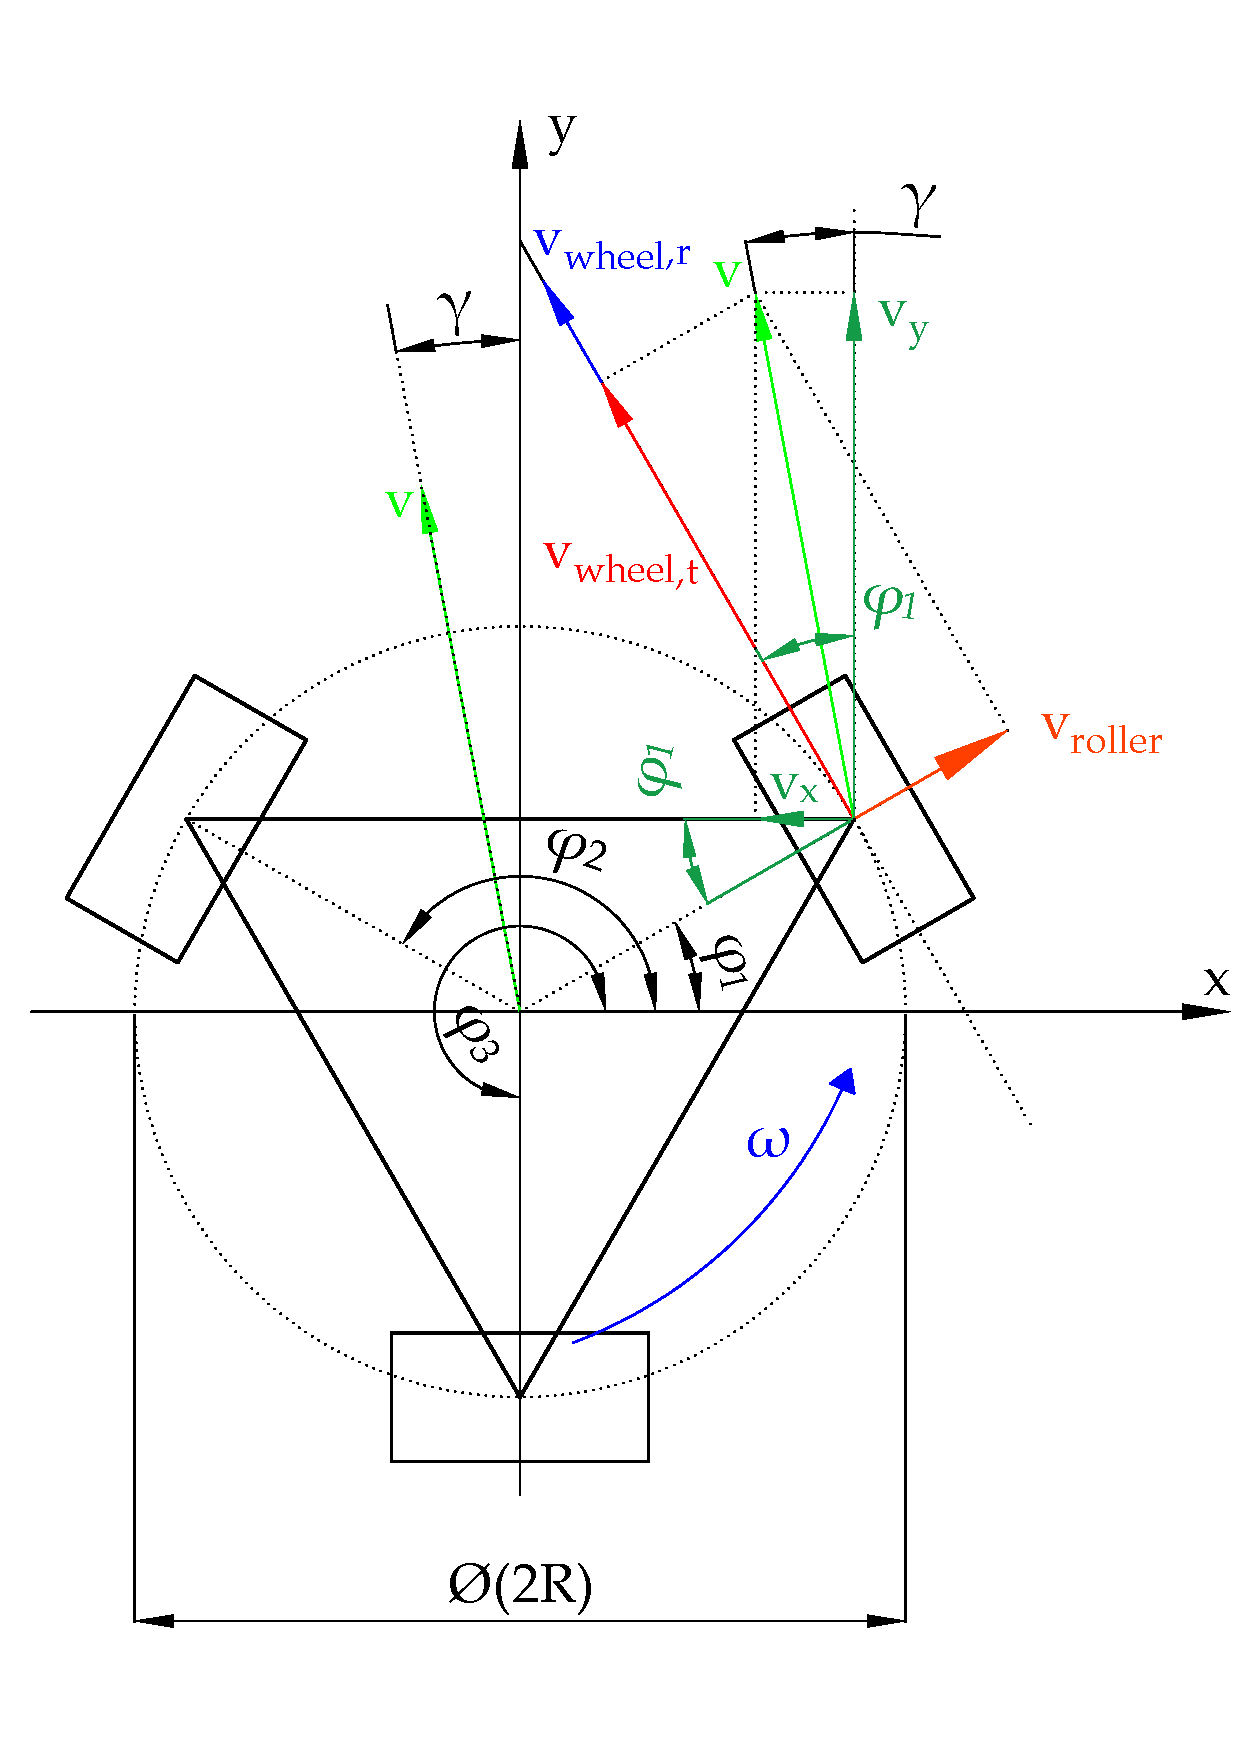
\includegraphics[width=7cm]{figures/omni_wheel_vectors}
	\caption{Wheel vectors in local (x,y) coordinate system}
	\label{omni_wheel_vectors}
\end{figure}

The omniwheels are located along the common wheel circle (R) at $\varphi_1, \varphi_2, \varphi_3$ angles measured from the local $x$ axis. The pure translational part of the wheel velocity can be written as a combination of the x,y components of the robot translational velocity as:
\begin{equation}
	{v_{wheel,t}}^i = - v_x sin \varphi_i  + v_y cos \varphi_i .
\end{equation}
Considering the equations above the total wheel velocity is:
\begin{equation}
	v_i = - v_x sin \varphi_i + v_y cos \varphi_i  + R \omega_i,
\end{equation}
therefore the angular velocity of the wheel is:
\begin{equation}
	\omega_i = \frac{1}{r} (- v_x sin \varphi_i + v_y cos \varphi_i + R \omega_i),
\end{equation}
which can be generalized in vectorial form as:
\begin{equation}
	\boldsymbol{\omega} = \mathbf{J^{-1}} \mathbf{v}
\end{equation}
\begin{equation}
\mathbf{v_i} = r \mathbf{J^{-1}} \mathbf{v} = \mathbf{T_{velocity}} \mathbf{v}
\label{velocity_tranformation}
\end{equation}

where
\begin{itemize}
	\item $\Omega = [\omega_1~\omega_2~\omega_3]^T$ is the wheel angular velocity vector,
	\item $\mathbf{J^{-1}}$ is the inverse Jacobian matrix of the case velocities which is
		\begin{eqnarray}
		\mathbf{J^{-1}}=\frac{1}{r} \left[
		\begin{array}{ccc}
		sin \varphi_1 & cos \varphi_1 & R \\
		sin \varphi_2 & cos \varphi_2 & R \\
		sin \varphi_3 & cos \varphi_3 & R \\
		\end{array}
		\right],
		\end{eqnarray},
	\item $\mathbf{T_{velocity}}$ is the velocity transformation matrix,
	\item $\mathbf{v} = [v_x~v_y~\omega]^T = [\dot x~\dot y~\dot \varphi]^T$ is the case velocity vector.
\end{itemize}
The inverse of determinant of J is never zero, thus its inverse always exists which means that kinematic relation between the wheels and the case is provided. In order to track the robot in the global configuration, the kinematic state has to be transformed from the local frame to the global frame which can be done by means of a simple rotation transformation perpendicular to (x,y) plane with $\alpha$ orientation angle:
\begin{equation}
\boldsymbol{x} = \mathbf{T}~\mathbf{X}\text{, i.e.}
\end{equation}
\begin{eqnarray}
\left[
\begin{array}{c}
\dot x \\
\dot y 	\\
\dot \phi \\
\end{array}
\right]=
\left[
\begin{array}{ccc}
cos \alpha 	& -sin \alpha & 0 \\
sin \alpha 	& cos \alpha & 0 \\
0	 		& 0 		 & 1 \\
\end{array}
\right]
\left[
\begin{array}{c}
\dot X \\
\dot Y 	\\
\dot \Phi \\
\end{array}
\right].
\end{eqnarray}
\subsubsection{2D Simulations}
Considering the equations above, a two-dimensional kinematic simulator was built-in Wolfram Mathematica which could help to understand more accurately the robot locomotion mechanism by calculating and then visualizing the movements. The simulator has to be initialized with as follows:
\begin{itemize}
	\item Common wheel circle (R) which is in this case: R = 0.12 m,
	\item Wheel position angles ($\varphi_i$) which is in this case $\varphi_1=30^{\circ}, \varphi_1=150^{\circ},\varphi_1=270^{\circ}$,
	\item Initial position and orientation $\mathbf{X} = [X~Y~\alpha]^T$, i.e. $\mathbf{p}=[X~Y]^T$ and $\alpha$,
	\item Initial velocity state in the local frame: $\mathbf{v} = [v_x~v_y~\omega]^T,$ i.e. $v,~\gamma$ and $\omega$.
	\item The solution is obtained numerically, integrating the velocities over time steps, thus timestep size ($dt$ )and simulation time (T) has to be provided.
\end{itemize}
The basic equations are the followings:
\begin{itemize}
	\item The new position equation is
	\begin{equation}
		\mathbf{p}^{i+1} = \mathbf{p}^{i} + \mathbf{T} \mathbf{v}^i dt,
	\end{equation}
	\item The new orientation equation is
	\begin{equation}
		\alpha^{i+1} = \alpha^{i} + \omega^i dt.
	\end{equation}
	\item The new velocity magnitude equation is
	\begin{equation}
		v^{i+1} = F(v^{i},dt,\mathbf{p}^{i},...).
	\end{equation}
	\item The new velocity direction equation is
	\begin{equation}
		\gamma^{i+1} = F(\gamma^{i},dt,\omega,...).
	\end{equation}
	\item The new angluar velocity equation is
	\begin{equation}
	\omega^{i+1} = F(\omega^{i},dt,\mathbf{p}^{i},...).
	\end{equation}
\end{itemize}

Figure \ref{relation_v_1_g_0_w_0} depict a pure translation in forward direction. An interesting characteristic of the robot configuration can be observed, i.e. the resultant case velocity can be greater than the wheel velocities. Figure \ref{relation_v_0_g_0_w_10} represent the case of pure rotation when the wheel velocities are equal.
\begin{figure}[htb!]
	\centering
	\minipage{0.5\textwidth}
	\centering
	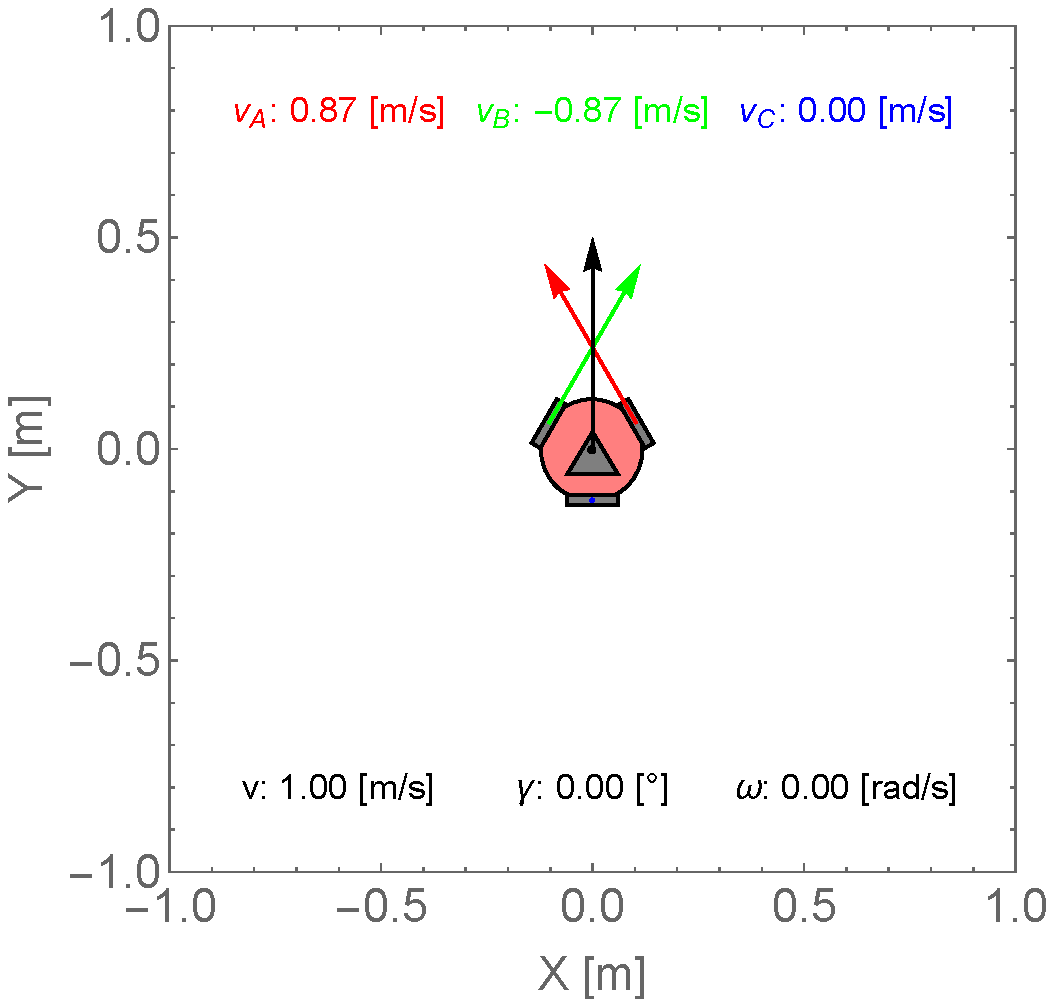
\includegraphics[height=7cm]{figures/2d_simulation/relation_v_1_g_0_w_0}
	\caption{Pure forward translation}
	\label{relation_v_1_g_0_w_0}
	\endminipage\hfill
	\minipage{0.5\textwidth}
	\centering
	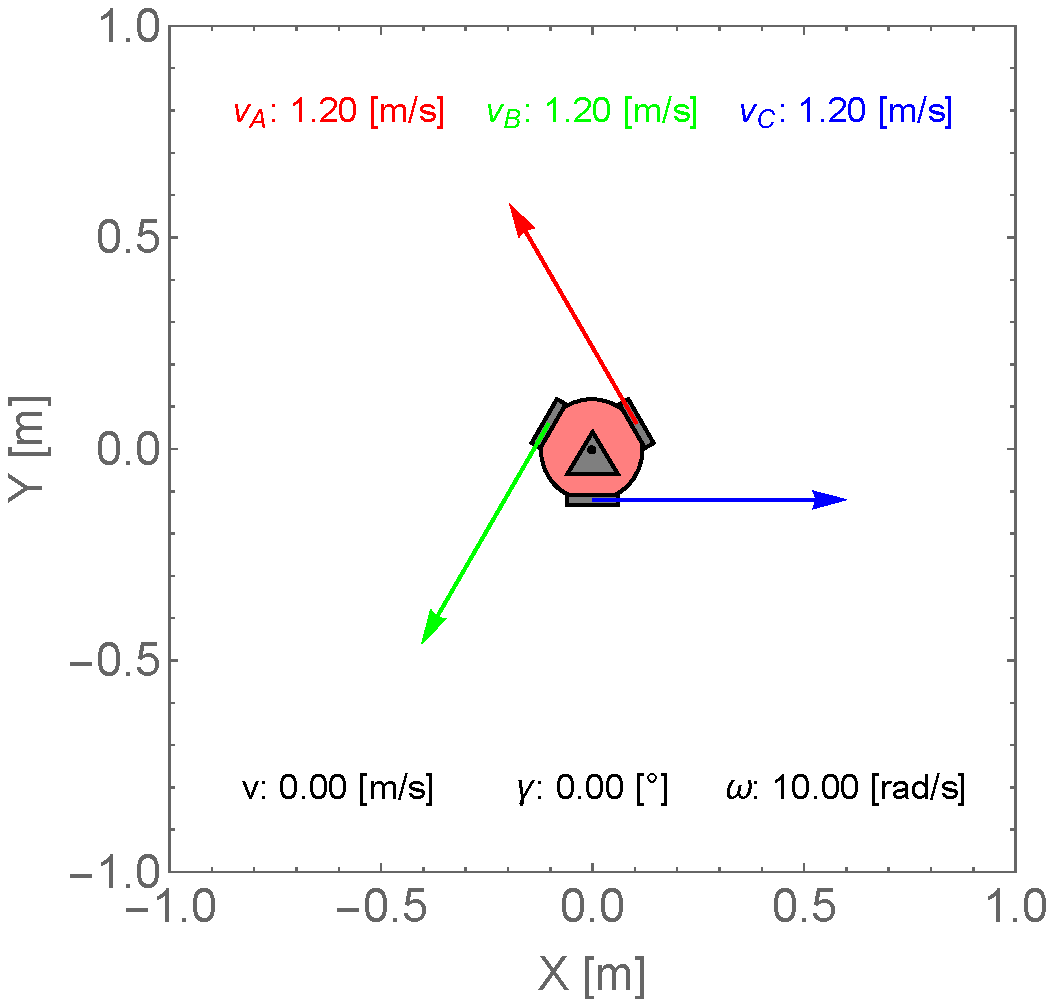
\includegraphics[height=7cm]{figures/2d_simulation/relation_v_0_g_0_w_10}
	\caption{Pure spinning}
	\label{relation_v_0_g_0_w_10}
	\endminipage\hfill
\end{figure}
Figure \ref{relation_v_1_g_30_w_0} depicts another specific case of pure translation when the velocity of wheel A equals the robot velocity, while the others drive with same speed but the opposite direction. Figure \ref{relation_v_06_g_45_w_6} represent a mixed case of translation in an arbitrary direction and rotation at the same time.
\begin{figure}[htb!]
	\centering
	\minipage{0.5\textwidth}
	\centering
	\includegraphics[height=7cm]{figures/2d_simulation/relation_v_1_g_30_w_0}
	\caption{Specific case of translation}
	\label{relation_v_1_g_30_w_0}
	\endminipage\hfill
	\minipage{0.5\textwidth}
	\centering
	\includegraphics[height=7cm]{figures/2d_simulation/relation_v_06_g_45_w_6}
	\caption{Translation \& rotation}
	\label{relation_v_06_g_45_w_6}
	\endminipage\hfill
\end{figure}
\newpage
The following figures represent the status of robots at given time steps during the simulations. The main equations that generates the shown motions are given. Generally there are 3 parameters to vary: the magnitude of the speed, the direction of the speed and the angular velocity.\\[0.3cm]
\noindent \textbf{Moving along a circle without changing the orientation:}
\begin{itemize}
	\item $dt=0.1~[\text{s}]$ (timestep size), $T=10~[\text{s}]$ (simulation time),
	\item $v^{i+1} = v^{i} = v^{0}$ (constant speed),
	\item $\omega^{i+1} = \omega^{i} = 0$ (no angular velocity),
	\item $\gamma^{i+1} = \gamma^i + \dot \gamma dt$ where $\dot \gamma = \frac{2 \pi}{T}$
\end{itemize}
\begin{figure}[htb!]
	\minipage{0.33\textwidth}
	\centering
	\includegraphics[height=5cm]{figures/2d_simulation/animations/2D_move_along_circle_not_rotating/20}
	\caption{$0.20[s]$}
	\endminipage\hfill
	\minipage{0.33\textwidth}
	\centering
	\includegraphics[height=5cm]{figures/2d_simulation/animations/2D_move_along_circle_not_rotating/40}
	\caption{$0.40[s]$}
	\endminipage\hfill
	\minipage{0.33\textwidth}
	\centering
	\includegraphics[height=5cm]{figures/2d_simulation/animations/2D_move_along_circle_not_rotating/60}
	\caption{$0.60[s]$}
	\endminipage\hfill
\end{figure}
The direction of the speed vector ($\gamma$) is defined in the local coordinate system and it has to be changed to make the robot move along a given curve, in this case along a circle.\\[0.3cm]
\noindent \textbf{Moving along a circle like a car (anholonomic):}
\begin{itemize}
	\item $dt=0.1~[\text{s}]$ (timestep size), $T=10~[\text{s}]$ (simulation time),
	\item $v^{i+1} = v^{i} = v^{0}$ (constant speed),
	\item $\omega^{i+1} = \omega^{i} = \omega^{0}$ (constant angular velocity),
	\item $\gamma^{i+1} = \gamma^i = 0$
\end{itemize}
\begin{figure}[htb!]
	\minipage{0.33\textwidth}
	\centering
	\includegraphics[height=5cm]{figures/2d_simulation/animations/2D_move_along_circle_rotating_car_like/20}
	\caption{$0.20[s]$}
	\endminipage\hfill
	\minipage{0.33\textwidth}
	\centering
	\includegraphics[height=5cm]{figures/2d_simulation/animations/2D_move_along_circle_rotating_car_like/40}
	\caption{$0.40[s]$}
	\endminipage\hfill
	\minipage{0.33\textwidth}
	\centering
	\includegraphics[height=5cm]{figures/2d_simulation/animations/2D_move_along_circle_rotating_car_like/60}
	\caption{$0.60[s]$}
	\endminipage\hfill
\end{figure}
\newpage
The following two cases are further demonstration of the fact that the orientation can be controlled independently from the linear motion, i.e. the robot has 3 DoF. \\[0.3cm]
\noindent \textbf{Moving along a circle changing the orientation in reverse direction:}
\begin{itemize}
	\item $v^{i+1} = v^{i} = v^{0}$ (constant speed),
	\item $\omega^{i+1} = \omega^{i}<0$ (angular velocity),
	\item $\gamma^{i+1} = \gamma^i + \dot \gamma dt -\omega^i dt$ where $\dot \gamma$ is a constant.
\end{itemize}
\begin{figure}[htb!]
	\minipage{0.33\textwidth}
	\centering
	\includegraphics[height=5cm]{figures/2d_simulation/animations/2D_move_along_circle_rotating_reverse_direction/20}
	\caption{$0.20[s]$}
	\endminipage\hfill
	\minipage{0.33\textwidth}
	\centering
	\includegraphics[height=5cm]{figures/2d_simulation/animations/2D_move_along_circle_rotating_reverse_direction/40}
	\caption{$0.40[s]$}
	\endminipage\hfill
	\minipage{0.33\textwidth}
	\centering
	\includegraphics[height=5cm]{figures/2d_simulation/animations/2D_move_along_circle_rotating_reverse_direction/60}
	\caption{$0.60[s]$}
	\endminipage\hfill
\end{figure}
In this case also the robot orientation and also the speed direction is changing from step to step. The changed orientation ($\omega dt$) has to be considered in the equation of $\gamma$ as being defined in the local frame.\\[0.3cm] 
\noindent \textbf{Moving along a line and changing the orientation:}
\begin{itemize}
	\item $v^{i+1} = v^{i} = v^{0}$ (constant speed),
	\item $\omega^{i+1} = \omega^{i}<0$ (angular velocity),
	\item $\gamma^{i+1} = \gamma^i -\omega^i dt$ where $\dot \gamma$ is a constant.
\end{itemize}
\begin{figure}[htb!]
	\minipage{0.33\textwidth}
	\centering
	\includegraphics[height=5cm]{figures/2d_simulation/animations/2D_move_along_line_and_rotating/20}
	\caption{$0.20[s]$}
	\endminipage\hfill
	\minipage{0.33\textwidth}
	\centering
	\includegraphics[height=5cm]{figures/2d_simulation/animations/2D_move_along_line_and_rotating/40}
	\caption{$0.40[s]$}
	\endminipage\hfill
	\minipage{0.33\textwidth}
	\centering
	\includegraphics[height=5cm]{figures/2d_simulation/animations/2D_move_along_line_and_rotating/60}
	\caption{$0.60[s]$}
	\endminipage\hfill
\end{figure}
The kinematic simulation code is a handy tool to demonstrate the possibilities of such a robot configuration, but it does not give any details from dynamics point of view. As it can be seen in previous chapter the real world is not as ideal, thus such a simple kinematic point of view is not enough to give a detailed analysis. These kinematic simulation assumes that the contacts are ideal and there are small accelerations, thus the wheels cannot slip.
\newpage
\subsection{Dynamic analysis of DC motors}
In order to have a proper dynamic model, the source of forces, i.e. the motors have to be analysed and modeled in details. As it was mentioned before, the permanent magnet type DC motors are easy to be described using 5 parameters (L,J,R,B,K), thus the primary goal is estimate these parameters.
\subsubsection{DC motor parameter identification}
The L (inductance) and J (second moment of inertia) describes the dynamic behavior of the motor, while the others characterize the system in a stationary aspect. Based on motor datasheet informations (no load case, max efficiency case, max power case, stall torque case), only the stationary parameters can be estimated and one can even not be sure about the values whether they match the reality or not. Obviously, to get know about the dynamic parameters, measurements of dynamic operations of the motors are needed, e.g. measuring the step response to a given function of voltage over time. A robust technique for the parameter identification is to combine the measurement results with the capabilities of MATLAB Simulink and its Design Optimization tool. To carry out the following models and the parameter identification process the following references were considered: \cite{par_est_1}, \cite{par_est_2},\cite{par_est_3}. The Simscape library of the Simulink makes it possible to make system models of coupled physical problems combining submodel elements, e.g. a DC motor which is an electromechanical system can be built using simple elementary mechanical and electrical components.

Firstly, in accordance with the equations of DC motor a basic model was made.
\begin{figure}[htb!]
	\centering
	\includegraphics[width=\textwidth]{figures/simulink_dc_motor.png}
	\caption{Simple DC motor electromechanical model in Simulink}
	\label{simulink_dc_motor}
\end{figure}

Figure \ref{simulink_dc_motor} represents the first model in which the blue is the electrical circuit consisting a resistance $(R)$, inductance $(L)$, DC voltage source, electrical reference and current sensor, while the green elements are mechanical blocks, i.e. the inertia $(J)$, rotational damper $(B)$, rotational reference and a rotational speed sensor. The interface between the two domains is provided by the electromechanical converter which defines the $K$ constant. The $f(x)$ block defines solver settings for the numerical solution and the other two elements are blocks that monitors the current and shaft speed over time. This model has to match with the governing equations because actually those are solved numerically. The armature current has high peeks at the starting of DC motors due to the absence of the back emf which is proportional with rotational speed. The high gradients make the equation system to be a stiff one, thus ode15s MATLAB solver's solution method was chosen which is a recommended one for such problems by means of the MATLAB help.

\begin{figure}[htb!]
	\centering
	\includegraphics[width=\textwidth]{figures/simulink_dc_motor_complex.png}
	\caption{Complex DC motor electromechanical model in Simulink}
	\label{simulink_dc_motor_complex}
\end{figure}
In order to use the parameter estimation tool of the software, more complex voltage inputs have to defined. This model works with simple constant DC input voltage only. From the Simscape library, further electrical components can be added to the model such as the H-Bridge which can switch the rotational direction of the rotor or such as the PWM module which can produce a square wave with a given duty cycle to control the magnitude of the input voltage. The model shown in Figure \ref{simulink_dc_motor_complex} has two inputs. One is the PWM reference signal which is a voltage value between 0 and 5V. The Controlled PWM unit generates from the reference signal a square wave which will be the input of the H-bridge motor drive component. This part can be related to a voltage value of PWM type digital pin of the MCU. The following component, the H-bridge motor drive, is actually the model of the L298N driver. The magnitude of its output voltage is controlled by the PWM signal's duty cycle, while that of polarity is controlled by the digital signal at REV port. The second input of the model is the Reverse Port Signal which has to be a digital signal, thus 0V (LOW) correspond to no polarity change and 5V (HIGH) corresponds to switched polarity, thus reverse rotation of the rotor. The output of the model is shaft speed considered in rad/s. Transient operation of the system is provided by changing the reverse port digital signal. 

In order to execute the parameter estimation with the specified inputs, measurements for the output speed had to be taken before the simulation could be run. In addition, the parameters has to be initialized in the model as a preliminary guess to have a combination of them to start the optimization from somewhere. Based the governing equations and motor data sheet values, a good initial guess could be given. In case of no load operation, $b=\frac{T}{\dot \theta}$ where $T=0.11$ [Nm] and $\dot \theta =11.21$ [rad/s] (107RPM), therefore $b=0.01[\frac{\text{Nms}}{rad}]$. Also other working points are known with respect to T-i values pairs, thus supposing linear relation the K can be estimated which was calculated to be 0.9338. Using these two values and supposing the steady state version of the Kirchoff law in case of no load, the resistance can be calculated as $R=\frac{V-K \dot \theta}{i} = 10.25$ [$\Omega$].
Considering all above, the initial guess of the seeked parameters is as follows:
\begin{equation}
\begin{split}
R=10[\Omega],~b=0.01[\frac{\text{Nms}}{rad}],~J=0.001[kgm^2],~L=0.01[H],~K=1[\frac{\text{Vs}}{rad}].
\end{split}
\end{equation}
\begin{figure}[htb!]
	\centering
	\includegraphics[width=\textwidth]{figures/simulink_par_est_1.png}
	\caption{Simulation results before and after the optimization}
	\label{simulink_par_est_1}
\end{figure}
 In the parameter estimation module both of the measurement and the simulation of the system can be represented which is shown in Figure \ref{simulink_par_est_1}. The plots on left side represent the simulation with the initial parameters. It can be seen that the steady-state value is close to the measured one, but the time constants are quite different. The plot on the right side correspond to the estimated values which are the followings:
\begin{equation}
\begin{split}
R=7.98[\Omega],&~b=0.0197[\frac{\text{Nms}}{rad}],~J=0.0121[kgm^2],\\
&L=0.166[H],~K=0.825[\frac{\text{Vs}}{rad}] 
\end{split}
\end{equation}
The sum of squared error was selected to be the cost function which converged from the initial value of 66.6 to 0.23 after 11 iterations. The obtained values are in a good relation with estimates, thus with the possible real values. The J and L changed drastically as they were estimated with arbitrary values since they cannot be estimated based on motor data sheet. The steady state current in the simulated free load case is 2 times higher, but the peak current is in a good order. Really high peaks can be got when the polarity of the input voltage is switched, therefore higher torques can be expected during such operations which means more risk for fall over for instance. The initial peak current can be estimated as $U/R = 12[V]/10.25[\Omega] = 1.17 [A]$ assuming zero initial shaft speed. Figure \ref{simulink_armature_current} shows a similar current peaks in the simulation.
 \begin{figure}[htb!]
 	\minipage{0.45\textwidth}
 	\centering
 	\includegraphics[width=\textwidth]{figures/simulink_par_est_2.png}
 	\caption{Iterations of estimated parameters}
 	\endminipage\hfill
 	\minipage{0.45\textwidth}
 	\centering
 	\includegraphics[width=\textwidth]{figures/simulink_armature_current}
 	\caption{Aramature current of the estimated model}
 	\label{simulink_armature_current}
 	\endminipage\hfill
 \end{figure}

The solution was obtained by means of numerical solution during the MATLAB simulations while the dynamic model of the robot can be solved analytically as well. Generally a more simple method is seeked that might be implemented also in the hardware code, thus it would be more convenient to find a good analytical formula too calculate the current, thus the motor torques exerted on the wheels and the rotational speed as well. 
The dynamic system model has the generic form is as follows:
\begin{eqnarray}
\left[
\begin{array}{c}
\dot \omega\\[2ex]
\dot i \\
\end{array}
\right]=
\left[
\begin{array}{ccc}
-\frac{b}{\theta } & \frac{k}{\theta } \\[2ex]
-\frac{k}{L} & -\frac{R}{L} \\
\end{array}
\right]
\left[
\begin{array}{c}
\omega  \\[2ex]
i 	\\
\end{array}
\right]
+
\left[
\begin{array}{c}
-\frac{T_{L}}{\theta}  \\[2ex]
\frac{V}{L} 	\\
\end{array}
\right] = 
\left[
\begin{array}{ccc}
a_1 & b_1 \\[2ex]
a_2 & b_2 \\
\end{array}
\right]
\left[
\begin{array}{c}
\omega  \\[2ex]
i 	\\
\end{array}
\right]
+
\left[
\begin{array}{c}
c_1  \\[2ex]
c_2 	\\
\end{array}
\right]
.
\label{dynamic_model_equation}
\end{eqnarray}
The Eq. \ref{dynamic_model_equation} is a system of two linear inhomogeneous first-order constant-coefficient ordinary differential equations. The solution of the homogeneous  part can be obtained by analyzing the characteristic equation of the state-space matrix. The characteristic equation can be derived by solving the eigenvalue problem and it is as follows:
\begin{equation}
\lambda^2-\lambda (a_1+b_2)+a_1 b_2 - a_2 b_1=0.
\end{equation}
which characteristic roots (eigenvalues) are:
\begin{equation}
\lambda_{1,2}=\frac{1}{2} \left({a_1}+{b_2} \pm \sqrt{({a_1}-{b_2})^2+4 {a_2} {b_1}}\right).
\end{equation}
In this case, the following conditions and that of consequences are present:
\begin{itemize}
	\item $a_1 b_2 - a_2 b_1 \neq 0$, thus the only stationary point is the origin of the state variables ($\omega,i$).
	\item The characteristic equation has two real negative distinct roots, thus it is asymptotically stable and the solution of the homogeneous has the following general form: \cite{eqworld}
	\begin{equation}
		\omega_h(t) = C_1 b_1 e^{\lambda_1 t} + C_2 b_1 e^{\lambda_2 t}
	\end{equation}
	\begin{equation}
		i_h(t) = C_1 (\lambda_1-a_1) e^{\lambda_1 t} + C_2 (\lambda_2-a_1) e^{\lambda_2 t}
	\end{equation}
	where $C_1$ and $C_2$ are initial condition dependent constants.
\end{itemize}
The inhomogeneous part does not change the system behavior it just shift the stationary point from the origin to another state ($\Omega_0$,$I_0$). The particular solutions are:
	$\omega_p(t) = \Omega,
	i_p(t) = I$
which can be calculated by means of system dynamic equations assuming a stationary form of it:
\begin{equation}
	a_1 \Omega + b_1 I + c_1 =0,
\end{equation}
\begin{equation}
	a_2 \Omega + b_2 I + c_2 =0.
\end{equation}
The general solution is the sum of the homogeneous and particular solution. Considering the initial conditions ($\omega_0,i_0$) and the applied motor voltage ($V$) and motor load torque ($T_L$) as parameters, it is possible to provide a closed-form expression for the armature current and rotor speed which are as follows after using the numerical values of the motor parameters got from the identification process:
\begin{equation}
\begin{split}
	\omega(t,V,T_L,\omega_0,i_0) = -9.52 T_L + 0.98 V + 
	&e^{-39.13 t} (-2.40 i_0 - 0.67 T_L + 0.37 V - 0.32 \omega_0) \\
	+&e^{-10.69 t} (2.40 i_0 + 10.19 T_L - 1.35 V + 
	1.32 \omega_0)
\end{split}
\end{equation}
\begin{equation}
\begin{split}
i(t,V,T_L,\omega_0,i_0) = -9.52 T_L + 0.02 V + 
&e^{-39.13 t} (1.32 i_0 + 0.37 T_L - 0.20 V - 0.18 \omega_0) \\
+&e^{-10.69 t} (-0.32 i_0 - 1.35 T_L + 0.18 V + 
0.17 \omega_0).
\end{split}
\end{equation}
The motor torque can be calculated as:
\begin{equation}
	T(t,V,T_L,\omega_0,i_0) = K i(t,V,T_L,\omega_0,i_0),
	\label{motor_load_equation}
\end{equation}
where 
	 $t~[\text{s}]$ is the time,
	 $V~[\text{V}]$ is the voltage,
	 $T_{L}~[\text{Nm}]$ is the load torque,
	 $\omega_0~[\text{rad/s}]$ is the initial shaft speed,
	 $i~[\text{rad/s}]$ is the initial armature current.
	 	 
The expressions are valid until the motor load torque, the supply voltage and the initial conditions of a given set of parameters are known. From practical point of view, it can be challenging to measure the armature current of a given state. As the electrical part has faster dynamics, it is a possible way of simplification to neglect the inductance of armature, in other words the inertia of the electric circuit. This will result that the armature current will reach its peak immediately.  With this assumption combining the two constitutive equations, the following first-order linear differential equation for $\omega[t]$ rotational speed can be derived:
\begin{equation}
	b \omega(t)+\theta \dot \omega(t)=\frac{K (V-K \omega(t))}{R},
\end{equation} 
which solution is:
\begin{equation}
	\omega(t) = \frac{e^{-\frac{b t}{\theta }-\frac{K^2 t}{\theta  R}} \left(K V e^{\frac{t \left(b R+K^2\right)}{\theta  R}}+b R \text{$\omega_0 $}+K^2 \text{$\omega_0 $}-K V\right)}{b R+K^2}
\end{equation}
where $\omega_0$ is the initial angular speed.
The armature current can be extracted as
\begin{equation}
	i(t) =\frac{V-K\omega}{R}.
\end{equation}
The motor torque can be calculated as:
\begin{equation}
T(t,V,T_L,\omega_0) = K i(t,V,T_L,\omega_0).
\end{equation}
Figure \ref{mahemetica_comparision_1} and \ref{mahemetica_comparision_2} depicts the two kind of analytical solutions for the shaft speed [rad/s] and armature current [A] where the orange solid line is the simplified analytic solution and dashed black is the general one. A simple accelerating from zero to max speed case is shown as a function of time.
 \begin{figure}[htb!]
	\minipage{0.48\textwidth}
	\centering
	\includegraphics[width=\textwidth]{figures/mahemetica_comparision_1}
	\caption{Angular velocity: (black - full solution, orange - simplified solution)}
	\label{mahemetica_comparision_1}
	\endminipage\hfill
	\minipage{0.48\textwidth}
	\centering
	\includegraphics[width=\textwidth]{figures/mahemetica_comparision_2}
	\caption{Armature current: (black - full solution, orange - simplified solution)}
	\label{mahemetica_comparision_2}
	\endminipage\hfill
\end{figure}
Regarding the shaft speed, the simplified approach is in an acceptable match with the more accurate one (where L is not assumed to be zero). One side, current peak, thus torque peak is at the very first moment and higher current is  estimated at start which is an conservative engineering approach, and less inputs are needed since the inductance is neglected. On the other hand, some details are lost for the simplicity what can be important in some cases. In this way, it is a good estimation to work with the simplified analytical formula as well if only simple trends and characteristics are seeked. For more detailed analysis, it is not recommended to neglect the armature inductance. 

The equations provided above are only valid until the system is treated as linear. If nonlinearities are present, the analytical solution likely does not exist. In case of such conditions, only the numerical solution of equations is feasible. Due to the stiffness of the system, a good strategy can be applying implicit Euler method combined with Newton-Raphson iteration for instance. For such a solution, the same inputs would be needed and the computational cost would be higher due to the increased number of expressions to be evaluated.

\subsubsection{Validation of the parameter estimation}
In the interest of validation of parameter estimation, a quite different case was investigated using the model and compared to measurements. It could be seen before that the motor does not work perfectly linear at lower voltages. Figure \ref{validation_figure} depicts the case of an acceleration with 50\%, 75\% and 100\% pwm signal from rest, then a braking with  0\%. The end speeds just before the change of the powering voltages are really the same. On the other hand, the simulation calculates faster dynamics at lower voltages and even at braking, but this can be regarded advantageous since it matches with the conservative engineering aspects. The estimated parameters can be accepted as they give quite good approximations at maximum acceleration states which are the most critical.

 \begin{figure}[htb!]
	\centering
	\includegraphics[width=0.6\textwidth]{figures/validation_figure}
	\caption{Validation of the identified parameters}
	\label{validation_figure}
\end{figure}
 \begin{figure}[htb!]
	\centering
	\includegraphics[width=0.6\textwidth]{figures/validation_figure_current}
	\caption{Armature current}
	\label{validation_figure_current}
\end{figure}


%%%%%%%%%%%%%%%%%%%%%%%%%%%%%%%%%%%%%%%%%%%%%%%%%%%%%%%%%%%%%%%%%%%%%%%%%%%%%%%%%%%%%%%%%%%%%%%%%%%%%%%%%%%%
% 											Mechanical model												
%%%%%%%%%%%%%%%%%%%%%%%%%%%%%%%%%%%%%%%%%%%%%%%%%%%%%%%%%%%%%%%%%%%%%%%%%%%%%%%%%%%%%%%%%%%%%%%%%%%%%%%%%%%%
\newpage
\subsection{Mechanical model of the robot}
A simplified dynamic model was made which is shown in Figure \ref{robotModel}. Its main purpose is to provide a tool that can evaluate the given states of the robot and estimate the risk for the fall over. The robot has a set of fixed properties, e.g. its geometry and inertias are known. As being a transport robot, it has a given payload which has to be taken to a destination without losing the stability. The package attached to the robot will change the mechanical properties and it can happen that it falls over if too high acceleration are caused. On one hand, this model is not aimed to describe the details of the fall over of the robot. In order to handle that process, a timed advanced solution should be provided by integrating the equations over time where due the change of the orientation around the global x and y axis, then the problem would became nonlinear and that of solution would be too time-demanding due to the extra calculation costs. The mechanical model should be much more detailed to capture properly the changing inertias of the robot, moreover the location of contact points would not be trivial to determine too. 

All in all, it would be too complicated and make no sense as it is not even wanted that the robot could work at the edge of its stability. From practical point of view, it is enough to search for an indicator that correlates well with the risk of fall over and try to avoid it by making predictions. For instance, monitoring the sign of the calculated normal force ($N_i$) between the wheels and the ground seems a reasonable choice. If its sign changes to negative from positive then the robot is possibly at edge of the fall over state. The negative sign has no real physical meaning since the ground contact is such a geometrical constrain that can only push but not pull. On the other hand, it is a really convenient and effective engineering approach to think as if it could work like that because then the closure of the system of equations is provided robustly and it is really simple to be solved.
 \begin{figure}[htb!]
	\minipage{0.5\textwidth}
	\centering
	\includegraphics[width=8cm]{figures/robotModel}
	\caption{Simplified mechanical model of the robot}
	\label{robotModel}
	\endminipage\hfill
	\minipage{0.5\textwidth}
	\centering
	\includegraphics[width=8cm]{figures/caseFBD}
	\caption{The case free body diagram}
	\label{caseFBD}
	\endminipage\hfill
\end{figure}
\subsubsection{Model of the robot platform}
The robot model shown in Figure \ref{robotModel} consists of the case, that of free-body diagram (FBD) is represented in Figure \ref{caseFBD} and three wheels which are shown in Figure \ref{wheelFBD} and \ref{wheelsFBD}. The wheels are connected to the case via simply joints which can transfer only force components, i.e. no moments. This means that also the moment pair of the motor torque is neglected hereby since its magnitude is about 1\% because of the gearbox which has a ratio of 1/90. In reality, it is exerted  due to Newton's 3rd Law on the motor housing, i.e. on the bracket which is connected to the case with screws. The origin ($r_O$) of the global frame is defined as a center of gravity of the wheel center points ($r_A,r_B,r_C$) when the orientation angle of the robot is zero, as in Figure \ref{robotModel} it is represented.
\begin{itemize}
	\item The levels of the robot configuration are considered as equilateral triangles. The second moment of inertia around the z axis of a single triangle at its own mass center can be calculated as $\theta_z=\frac{m R^2}{3}$ where $R=0.12~\left[\text{m}\right]$ is the common wheel radius. The other components of the inertia matrix is calculated as if it was a disk for simplicity. As it was mentioned, the fall over is not calculated, thus these components are ignored in later the calculation as they are actually not used, only the z component is important. On the other hand, the equations of Newton's 2nd Law are formulated in a general form for keeping the possibility for future modeling extensions.
	\item The motors and that of brackets are considered as point masses at the wheel center points.
	\item The package is considered as a (set of) cylinder shape object having $\theta_z=\frac{m_p r_p^2}{2}$. The contact between the case and the package is bonded.
\end{itemize}

The equations of Newton's 2nd Law at common center of mass for the robot case are as follows:
\begin{equation}
	m_R \mathbf{a} = \mathbf{K_A} + \mathbf{K_B} + \mathbf{K_C} + \mathbf{G}
\end{equation}
where \begin{itemize}
	\item $m_R~[\text{kg}]$ is the common mass of the case and the package,
	\item $\mathbf{a}~[\frac{\text{m}}{\text{s}^2}]$ is the acceleration vector,
	\item $\mathbf{K_i}~[\text{N}]$ is the force transfered at wheel connections, i=[A,B,C],
	\item $\mathbf{G}~[\text{N}]$ is the weight force, $G=-g m_C$ where $g=9.81~[\frac{\text{m}}{\text{s}^2}]$ is the gravitational body force. $\mathbf{G}=-G \mathbf{u}$ where $\mathbf{u}$ is a unit vector pointing in negative z direction.
\end{itemize}
\begin{equation}
\boldsymbol{\theta_R} \boldsymbol{\varepsilon} +\boldsymbol{\omega} \times (\boldsymbol{\omega} \times \boldsymbol{\theta_R \boldsymbol{\omega}}) = (\mathbf{r_A}-\mathbf{r_{CoM}}) \times \mathbf{K_A} + (\mathbf{r_B}-\mathbf{r_{CoM}}) \times \mathbf{K_B} + (\mathbf{r_C}-\mathbf{r_{CoM}}) \times  \mathbf{K_C}
\end{equation}
where \begin{itemize}
	\item $\boldsymbol{\theta_R}~[\text{kg m}^2]$ is the common second moment of inertia matrix at the center of mass (CoM), $\boldsymbol{\theta_R} = \boldsymbol{\theta_{Case}} +\boldsymbol{\theta_{Package}} + \boldsymbol{\theta_{MotorA}} + \boldsymbol{\theta_{MotorB}} + \boldsymbol{\theta_{MotorC}} $ (each inertia matrix of a given body is calculated at its own center of mass and then transformed to the common  center of gravity),
	\item $\boldsymbol{\varepsilon}~[\frac{1}{\text{s}^2}]$ is the angular acceleration  vector,
	\item $\boldsymbol{\omega}~[\frac{1}{\text{s}}]$ is the angular velocity vector,
	\item $\mathbf{r_A},\mathbf{r_B},\mathbf{r_C}$ are the wheel position vectors and $\mathbf{r_{CoM}}$ is the position vector of the common center of mass which is
	\begin{equation}
		\mathbf{r_{CoM}} = 
			\frac{
				m_{Triangle} (\mathbf{r_1}+\mathbf{r_2})		+
				3 \times m_{Motor} \mathbf{r_O}					+
				m_{Others} \frac{(\mathbf{r_1}+\mathbf{r_2})}{2} 			+ 
				m_{Package}
				\mathbf{r_{Package,CoM}}
			}{
				m_{Case}+m_{Package}
		}
	\end{equation}
	where \begin{itemize}
		\item $m_{Case} = 2 \times m_{Triangle} + 3 \times m_{Motor} + m_{Others}$,
		\item $m_{Triangle} = 0.184~[\text{kg}]$ is the mass of the triangle-shaped case elements,
		\item $m_{Motor} = 0.200~[\text{kg}]$ is the mass of the motor and the bracket,
		\item $m_{Others} = 0.4~[\text{kg}]$ is the mass of the other electronic hardware elements which are considered as if it was in the center of mass of the triangles,
		\item $m_{Package}$ is the arbitrary mass of the package.
	\end{itemize}
\end{itemize}
The are 15 unknowns while 6 equations are known up to this point: \begin{center}
	$a_x,a_y,a_z,\varepsilon_a,\varepsilon_b,\varepsilon_c,{K_x}^A,{K_y}^A,{K_z}^A,{K_x}^B,{K_y}^B,{K_z}^B,{K_x}^C,{K_y}^C,{K_z}^C$.
\end{center}
The mechanical equations are considered for each wheels in their local coordinate system which definition is depicted in Figure \ref{wheelsFBD}. 
\begin{figure}[htb!]
	\minipage{0.45\textwidth}
	\centering
	\includegraphics[height=8cm]{figures/wheelsFBD}
	\caption{The free-body diagrams of the wheels}
	\label{wheelsFBD}
	\endminipage\hfill
	\minipage{0.45\textwidth}
	\centering
	\includegraphics[height=8cm]{figures/wheelFBD}
	\caption{The free-body diagram of the wheel A}
	\label{wheelFBD}
	\endminipage\hfill
\end{figure}

Applying the Newton's 3rd Law and taking into consideration the given coordinate system tranformations, the following relationship can be written  regarding the transfered forces in the joints:
\begin{equation}
\mathbf{k_i} = -\left[
\begin{array}{ccc}
cos (-\varphi_i) 	& -sin (-\varphi_i)  	& 0 \\
sin (-\varphi_i)  	& cos (-\varphi_i)  	& 0 \\
0	 			& 0 				& 1 \\
\end{array}
\right] \mathbf{K_i} = \boldsymbol{\sigma_i} \mathbf{K_i}
\end{equation}
where $\mathbf{k_i}$ is the force in the joint in the local wheel frames and $i=[A,B,C]$. $\boldsymbol{\sigma_i}$ is the rotational transformation matrix between the global and local frame. In other words, the components of $\mathbf{k_i}$ will not be new unknowns having the relationship above. Beside the forces in the connection, the gravitational body force and the contact forces ($N,S$) are considered in case of the wheels to be pointing in pure y,z directions respectively. \cite{csernak} As a rough approximation, simple one-point contact and no slip condition is assumed which provides six kinematic constrain equations:
\begin{flalign}
{a_y}^i&=-r{\varepsilon_y}^i\\
{a_z}^i&=0
\end{flalign}
where $i=[A,B,C]$.\\
In the axial direction the moving friction force is not considered. In reality in case of an omni wheel, there are rollers in a circumferential alignment which can also spin. In this model, they are modeled as simple frictionless sliders. The possibility of the slippage of wheels are neglected as it would need precise measurements to have a dynamic friction coefficient. On the other hand, the so called rolling resistance can be defined as an adverse torque from the motor load torques ($M^i$) point of view which could be taken into consideration in the DC motor equations as loads.\\
The Newton equations for the wheels ($i=[A,B,C]$) are the followings:
\begin{equation}
m_i \mathbf{a_i} = \mathbf{k_i} + \mathbf{S_i} + \mathbf{G_i} + \mathbf{N_i}
\end{equation}
where \begin{itemize}
	\item $\mathbf{k_i}~[\text{N}]$ is the force transfered by the joint,
	\item $\mathbf{S_i}~[\text{N}]$ is the static friction force,
	\item $\mathbf{G_i}~[\text{N}]$ is the gravitational force,
	\item $\mathbf{N_i}~[\text{N}]$ is contact force.
	\item $m_i  = 60~[\text{g}]$ is the mass of a single wheel,
	\item $\mathbf{a_i}~[\frac{\text{m}}{\text{s}^2}]$ is the acceleration,
\end{itemize}
\begin{equation}
\boldsymbol{\theta_i} \boldsymbol{\varepsilon_i} +\boldsymbol{\omega_i} \times (\boldsymbol{\omega_i} \times \boldsymbol{\theta_i \boldsymbol{\omega_i}}) = - \mathbf{M_i} + \mathbf{r_{S_i}} \times \mathbf{S_i}
\end{equation}
where \begin{itemize}
	\item $\boldsymbol{\theta_i}~[\text{kg m}^2]$ is the second moment of inertia matrix of the wheel at the center of mass (CoM), its axial (x) component comes from the DC parameter identification, i.e. the total inertia of the rotating part is considered.
	The other components are calculated as if it was a cylinder with the known geometry and mass. This simplification is acceptable because of the fact that the fall over is not wanted to be treated by the model but the general three-dimensional modeling equations are considered
	\item $\boldsymbol{\varepsilon_i}~[\frac{1}{\text{s}^2}]$ is the angular acceleration of the wheel,
	\item $\boldsymbol{\omega_i}~[\frac{1}{\text{s}}]$ is the angular velocity of the wheel,
	\item $\mathbf{M_i}$ is the resultant torque exerted on the rotating part of the motor and the wheel. It is the sum of the motor torque and the adverse friction torques.
	\item $\mathbf{S_i}$ is the static friction force at the contact of the wheel and ground, while $\mathbf{r_{S_i}}$ is the vector pointing to the contact point from the wheel center of mass $(\mathbf{r_{i}})$.
\end{itemize}
There are 24 additional unknowns which are the followings:
\begin{center}
	${a_x}^i,{a_y}^i,{a_z}^i,{\varepsilon_x}^i,{\varepsilon_y}^i,{\varepsilon_z}^i,S^i,N^i$ where $i=[A,B,C]$.
\end{center}
The Newton's 2nd Law provides 24 equations (6 for each wheels), the rolling constrains means 6 equations, thus in order to have the closure of the system 6 more equations are needed.
The wheel-case joint can be assumed to be a rigid body connection in which case the following equations stand and make the closure:
\begin{equation}
	\mathbf{a_i} = \boldsymbol{\sigma_i} (\mathbf{a}+\boldsymbol{\varepsilon} \times \mathbf{r_i}+\boldsymbol{\omega} \times (\boldsymbol{\omega} \times \mathbf{r_i})).
\end{equation}

The motor loads can be calculated by means of the Eq. \ref{motor_load_equation}, thus the coupling can be done leading to an electrodynamic model. The simplified analytic approach can be used as weel as that is an overestimation due to the higher angular acceleration peaks, faster as only the evaluation of an analytic formula at t=0 is needed. The search of the peak is not needed since the current considered to reach its peak at the very first moment, thus the peak moment estimation is possible without having to know the preceding armature current as an initial condition. 

Eventually, the inputs of the model are inertias of components (mass, second moment of inertia), motor velocity states and the voltages at the pins of the motors, meanwhile the output is the acceleration state of the entire robot. The desired voltages can be determined by means of the velocity transformation matrix derived in the previous chapter (see Eq. \ref{velocity_tranformation}) which was about the kinematics. This can be generalized since the wheel speed is proportional with the applied voltage, therefore a prescribed motion can be carried out by applying the voltages in the same ratio as in an idealistic model the velocities should be applied.

\subsubsection{Simulations of motor states}
Figure \ref{accelerationState} represents a solution of a simple forward acceleration case from rest. It can be seen that the contact forces of wheel A,B decreases while that of wheel C increases. This phenomenon can be explained by the inertial forces which tries to rotate the case and at the same time the increased contact forces withstand in order to prevent the rotation. In case of too high acceleration compared to the height and the inertias of robot, this phenomenon could lead to fall over. 
If the magnitude of acceleration is kept constant, the corresponding distribution of contact forces will depend on the direction of the acceleration vector.
Figure \ref{dangerousOri} depicts the parametric solution of the contact forces with respect to the $\gamma$ angle of the acceleration vector. The dependence can be described with trigonometric functions and it can be concluded that the most dangerous cases, i.e. minimum values of contact forces are present when the robot accelerates such a way that the direction of the acceleration vector is coincident with a single wheel direction. It is possible that by changing only orientation of the robot, the model equations calculates negative contact forces. As it was mentioned, negative forces have no real physical sense, they are just obtained because of the special kinematic constrains but they can be regarded as an indicator for a possible risk for fall over. The ground constrain works as if it was able to exert pulling force to prevent the rising of the case. It can be an unexpected problem when the robot tries to move along a curved path and the so called centrifugal acceleration has the robot lost its stability. A possible safety feature can be for such a robot to change its own orientation along the curve so that it takes into consideration the direction of the current acceleration and tries to set such an own orientation where the reduction of contact forces are equally distributed between two wheels instead of one as in the worst case. The angular acceleration does not affect the contact forces based on this model, thus such movements for correction purposes can be done safely and independently having three degrees of freedom.
\begin{figure}[htb!]
	\minipage{0.45\textwidth}
	\centering
	\includegraphics[height=7cm]{figures/accelerationState}
	\caption{State at forward acceleration in the safest orientation in terms of contact forces as the reduction is distributed between two wheels}
	\label{accelerationState}
	\endminipage\hfill
	\minipage{0.45\textwidth}
	\centering
	\includegraphics[height=7cm]{figures/dangerousOri.png}
	\caption{The free-body diagram of the wheel A}
	\label{dangerousOri}
	\endminipage\hfill
\end{figure}

Figure \ref{accelerationState} depicts the case with the most favorable orientation with respect to the evolution of the contact forces. Despite the fact that this model could predict a risk for fall over even in this configuration, in the reality this can hardly happen. In this case the wheel A and B could rise above the ground due to the too high acceleration but as they are actually the ones that causes the accelerations also the cause would vanish. Moreover, the wheel C is just perpendicular to the direction of the acceleration, thus its passive rollers are aligned such a way that they can roll freely. The direction of the rolling just after the rising of the wheels, thus the rotation of the robot depends on the location of the common center of mass. Figure \ref{fallover_ppt} shows the two possible cases. On one hand, the gravitational force is always balanced by the contact force on the passive wheel. On the other hand, the resultant moment, thus the direction of the angular acceleration depends on the orientation of the geometry, i.e. the relative position of center of mass referenced to the passive wheel contact point. If the robot case does not rotate that much that the center of mass could get beyond the passive wheel, then the robot will fall back and roll towards the passive wheel. Therefore, the opposite situation can not even happen by an inertial force which is caused by a too high acceleration as the passive will roll in the opposite direction immediately after the contact of wheel A and B are lost. Although, in reality there are mostly such conditions when this prediction based on this given idealistic model does not hold properly. The case is not perfectly rigid, thus it will vibrate and it may deform such a way due to a sudden inertial force that the center of mass can get beyond the wheel. In addition, the passive wheel can also stick to a given surface if it is not perfectly aligned or the passive roller does not work as an idealistic roller, i.e. as a slider from global point of view if the moving friction is not considered.
\begin{figure}[htb!]
	\centering
	\includegraphics[height=6cm]{figures/fallover_ppt}
	\caption{Dependence of the location of center of mass}
	\label{fallover_ppt}
\end{figure}

In any kind of other situation, the robot can theoretically fall over even in this configuration if it gets a specific amount of angular momentum by an external disturbance. In that case, the resultant of the obtained angular momentum and the effect of the gravitational torque will determine whether it falls over or not. This problem is highly nonlinear due to the change of orientation and needs a time-advancing solution to have analysis about the possible outcome, which is here not the goal to deal with.

There can be cases when the orientation of the robot cannot be changed or simply not changed for any reason and the acceleration of the robot is oriented in the most disadvantageous direction. It is disadvantageous from the certain perspective that this is the direction in which the robot can loose stability more easily due to the alignment of the driving wheels, i.e. the robot can tilt itself by exerting hight torques on the driving wheels as the driving wheels keep their contact with the ground during the fall over as well. Using the derived model an autonomous robot can predict for a given input if too high accelerations are expectable and control the motors to avoid the risky manoeuvres. 

Let us consider that the given robot has a disk shaped mass on a rod which is bonded to the case just as in Figure \ref{fallover_ppt}. This construction was motivated by only demonstrative reasons as it could be realized in my hardware configuration as well using a threaded rod and disk shaped weights. If the resultant center of mass is located at a higher vertical level, the motor will more likely fall over for the same accelerating torques. In order to raise the center of mass point, added extra mass above the robot center of mass is needed. Needed means in this case, the need for the analysis to have a configuration that generally operates at the edge of its own stability in certain events and then it may tries operate such a way to avoid the possible risks. A possible case can be when the robot moves with a constant speed using two driving wheels just in the risky orientation then suddenly the driven wheels are braked by applying a voltage step from a given constant value to zero. The robot starts deccelerating and the inertial force tries to lean it over. By the way, this is more or less equivalent case to a constant acceleration from rest in the opposite direction.

\begin{figure}[htb!]
	\minipage{0.45\textwidth}
	\centering
	\includegraphics[height=7cm]{figures/draw_robot_baking}
	\caption{Peak state at braking in case of most disadvantageous orientation when the contact force reduction is concentrated on a single passive wheel}
	\label{draw_robot_braking}
	\endminipage\hfill
	\minipage{0.45\textwidth}
	\centering
	\includegraphics[height=7cm]{figures/draw_robot_accelerating}
	\caption{Peak state at accelerating in case of most disadvantageous orientation when the contact force reduction is concentrated on a single passive wheel}
	\label{draw_robot_accelerate}
	\endminipage\hfill
\end{figure}
The peak points for the two equivalent (and most dangerous) acceleration states are represented in Figure \ref{draw_robot_braking} and \ref{draw_robot_accelerate}. It can be seen that the same peak contact forces are calculated by the model. To have a more detailed view, using the simplified analytic model simulations were made for the problematic orientations.
Figure \ref{braking_1_0_kg_1_0_m} shows that in case of max braking power, the simplified model predicts negative contact forces for the passive wheel with the given inertias. Applying a smaller voltage step to a non zero initial value then decreasing that of value exponentially provides a smooth and not risky acceleration. The simulation in case of negative contact forces are strictly invalid as the ground cannot pull, they are just a simplified tool for prediction of fall over. If no negative contact forces in the simulation are captured, then the obtained characteristic can be regarded as an estimation having similar trend of the real ones, i.e. physical quantities change by exponential trend if idealistic - linear - conditions are assumed. In reality, the wheel speed reaches the constant zero value earlier due to the presence of static friction.
\begin{figure}[htb!]
	\centering
	\includegraphics[width=\textwidth]{figures/braking_1_0_kg_1_0_m}
	\caption{Braking with max torque and reduced torque in case of 1.0[kg] disk at the top of the rod at 1[m] height}
	\label{braking_1_0_kg_1_0_m}
\end{figure}

It is important to emphasize that the presence of the negative forces does not guarantee that the robot will fall over. If the negative forces last for only moments, in other words the passive wheel is not in contact with the ground anymore, there will not be enough work from driven wheels to overcome the reversing torque exerted by the gravitational force. Eventually, it can be concluded that all in all it can be a conservative engineering approach to tune the braking profile such a way that no negative forces could be calculated by the model. The tuned voltage profile in the simulation is obtained such a way that resultant torque profile is the one-third of the maximal one at each time step, thus automatic and smooth decrement is also set at the same time. If mass of the disk or that of position along the rod or the length of the rod changes, this calibration will likely not work. If only the mass of the disk is the changing variable in the system, then combining the above force prediction model with a mass estimator one, a more general prediction tool can be got.
\subsubsection{Comparision with measurements}
In order to test the derived dynamic model whether it is in a good relation with the reality or not, measurements were held using the built robot configuration. The robot started to move from rest and reached its maximum speed under $2$ [s] then stopped applying a step to zero voltage with a steep falling edge resulting in a high torque on wheels, thus high acceleration at the center of gravity of the whole configuration. In order to shift the center of gravity in a higher position, a threaded rod was applied with an additional disk-shaped masses attached to the end. The order of the center of mass displacement can be controlled by applying higher mass at the top as well. 

The configuration with the rod that has $0.373$ [kg] mass and is attached by a disk that has $0.5$ [kg] mass, was proven to be able to resist the braking condition which is shown in Figure \ref{fallover_video_05kg}.
\begin{figure}[htb!]
	\centering
	\includegraphics[width=\textwidth]{figures/fallover_video_05kg.png}
	\caption{Braking with max torque in case of 0.5[kg] disk at the top of the rod at 1[m] height; the passive wheel loose the contact with ground, then it falls back since not enough work is done by the inertial forces}
	\label{fallover_video_05kg}
\end{figure}
 The single passive wheel rose above the ground slightly but the robot's center of gravity did not rotated beyond the passive wheel, therefore it returned to the ground after some oscillatory bouncing. From practical point of view, this behavior is also undesired since it is a risky way of stopping and such movements can cause damages. Then, the mass at the top was doubled and the robot fell over without any doubts which is shown in Figure \ref{fallover_video_1kg}. 
 \begin{figure}[htb!]
 	\centering
 	\includegraphics[width=\textwidth]{figures/fallover_video_1kg.png}
 	\caption{Braking with max torque in case of 1.0[kg] disk at the top of the rod at 1[m] height; the robot with the doubled mass at top clearly falls over due to the its linear momentum}
 	\label{fallover_video_1kg}
 \end{figure}

After the video measurements, the simplified time advanced solution of the more detailed analytical expression were performed as well. The dynamic model provided an initial peak of passive wheel contact force of -5.02[N] for 1[kg] and -0.68[N] for 0.5[kg]. The derived dynamic model predicted negative forces, thus passive wheel rising which was experienced during the measurements as well. It is also favorable that the same tendency was captured which also a good verification of the model. From engineering point of view, the model provides estimation of fall over risk in a conservative manner if avoidance of negative signs of contact forces is the main design challenge.

\begin{figure}[htb!]
	\centering
	\includegraphics[width=\textwidth]{figures/simulation_0_5_1_0}
	\caption{Braking simulations (left: 0.5kg, right: 1.0kg)}
	\label{simulation_0_5_1_0}
\end{figure}

With the given weights also the fall over was tested in case of opposite direction acceleration, i.e. in such configuration when the contact force distribution is theoretically the most favorable, see \ref{accelerationState} As it was mentioned, the simplified rigid and one-point contact robot model automatically predicts that it impossible to happen. With the given weights it was unable to fall over in the measurements. Just after the braking, the two driven wheels rose above the ground for a little time then fell back. Due to the intense vibration of the rod, the robot changed a random amount of its orientation angle in clockwise or counter-closckwise direction by rotating around the third passive wheel's contact point(s). On one hand, it was verified by the measurement that the robot can fall over in a specific direction and it cannot do like that in the corresponding opposite direction if the same inertias and accelerating power is used. On the other hand, due to the undesired random rotation around the passive wheel, the robot changes its orientation a little bit which is likely not acceptable in a real-life situations. Consequently, working at the edge of stability in this case is also a state which is wanted to be avoided during operation since it can lead to inaccurate orientation control and unpredicted movements. 

Generally, the contact force depends on the mass of the attached disk and that of height of attachment in case of a given robot configuration and the acceleration state. 
\begin{figure}[htb!]
	\centering
	\includegraphics[height=5.5cm]{figures/contactForce2D_2}
	\caption{Passive wheel contact force (red means positive)}
	\label{contactForce2D}
\end{figure}
Figure \ref{contactForce2D} represents the contact force of the passive wheel during the braking case as a function of the disk mass and height of attachment. It can be seen that by increasing either of them causes a reduction of contact force, thus increased risk for fall over.


In this demonstrative configuration, it can be said that the height of the attachment point of the disk is kept constant, then only the disk mass remains as an unknown if the acceleration state is known.
\subsubsection{Mass estimation}
A more general model can be developed if a mass estimation algorithm is provided too. For instance, the acceleration of the robot case has to depend on the robot mass. Although, the dependence is not trivial as the common acceleration is the resultant of three accelerating wheels. Parametric solution for the initial acceleration in case of the braking is shown in Figure \ref{massDep} using the simplified analytical approach. Compared to the weight of the robot (which is about 2[kg]), a quite high mass of payload is needed to have noticeable difference in the initial acceleration peak. In this consideration the rolling friction is not included, the acceleration dependence is caused by changes of inner joint force components which depends on the case mass. In my case, the robot hardware was able to have extra load about 2[kg] without having too high case deformations that can be harmful, therefore this configuration is probably not able to work in a range where remarkable derivatives of the acceleration state could be experienced. Another problem is that the peak is not at the very first moment of an accelerating process which makes it harder to find the peak amplitude time. Additionally, the height of the peak is hard task to measure accurately using the rotary encoder since it uses double differentiation.
\begin{figure}[htb!]
	\minipage{0.45\textwidth}
	\centering
	\includegraphics[height=7cm]{figures/massDep}
	\caption{Mass of payload dependence of acceleration state}
	\label{massDep}
	\endminipage\hfill
	\minipage{0.45\textwidth}
	\centering
	\includegraphics[height=7cm]{figures/epsilonCompare}
	\caption{Comparision of angular accelerations of the motors}
	\label{epsCompare}
	\endminipage\hfill
\end{figure}

Figure \ref{epsCompare} represents measurement and simulation results of a no load case for a motor. It is enough to analyze a single wheel dynamics as the linear acceleration of the case is a definite resultant of wheel states. The pure measurement is quite noisy as so high accelerations are calculated even if the the velocity of the wheel is constant. A moving average filter was tested to make some corrections on the data. If averaging is taken on the two previous and proceeding timesteps (MA4) then the oscillation in case of steady state vanishes and the peak gets closer to the simulated ones. On the other hand, also the peak time is shifted which originally matches quite well with the numerical simulation. Same tendency can be experienced with a longer averaging function (MA10). Then the same measurements were carried out with package loads up to ~1.7 [kg]. As it was mentioned, for structural reasons it was the maximum that this simple mobile robot could hold without harmful deformations. The measurements results showed little difference regarding the wheel accelerations. As in Figure \ref{massDep} shown, the relative changes of the initial peak of linear acceleration as a function of payload of the given robot hardware is too small compared to the measurement and processing errors (numerical differentiation) of the rotary encoders. It can be stated that the errors are more significant then the sensitivity to the payload mass, therefore monitoring the acceleration state is not suitable for developing a mass estimator algorithm. 

Considering all above, a static approach was used in the end. In the equations, only viscous resistance was considered. In reality, there is no one-point contact between a wheel and ground. Both of the contact surfaces will deform and have multiple contact points which will exert adverse torque on the wheel, therefore additional torque is needed for keeping a constant speed beside the viscous resistance. The magnitude of the rolling resistance torque basically depends on the mass of the robot, the wheel and surface material characteristic since these will determine the degree of deformation of the contact surfaces. It can be generally written as $M_r = \mu_r m g$ where $\mu_r$ is the rolling resistance coefficient. From the motor point of view, it can be handled as a constant motor load which appears if the wheel is in contact with a surface and wants to roll. Therefore, beside the dynamic behavior also the final speed of the motors will be different, actually in a proportional way with the robot mass which can be utilized for a mass estimation algorithm.
The final speed measurements with different added extra masses (0g, 500g, 1000g, 1500g, 2000g) were performed. All the wheels were powered by the maximal 12V, therefore the robot was spinning around its own axis. This is an advantageous movement since as it was mentioned, the only spinning case does not change the contact forces, thus it is a safety way of measuring an unknown added mass. When the transient state at the beginning was finished, the final speeds were calculated by averaging the speed data for some seconds. Using the 0g, 500g and 2000g measurement averaged speed data a linear curve was fitted to have a estimator function in such a way that the no mass case perfectly align with the curve. Let us suppose that the cases of 1000g and 1500g extra mass are unknown mass measurements and one wants to estimate the unknowns based on the fitted curve of the three known mass measurement casess (0g, 500g and 1000g extra masses). The measurement data with relative velocities scaled by the maximal 0g speed and the fitted curves are shown in Figure \ref{rolling_fric_meas} and the corresponding relative errors of the estimator function is shown in Figure \ref{mass_estimate}.
\begin{figure}[htb!]
	\minipage{0.45\textwidth}
	\centering
	\includegraphics[height=7cm]{figures/rolling_fric_meas}
	\caption{Mass of payload dependence of acceleration state}
	\label{rolling_fric_meas}
	\endminipage\hfill
	\minipage{0.45\textwidth}
	\centering
	\includegraphics[height=7cm]{figures/mass_estimate}
	\caption{Comparision of angular accelerations of the motors}
	\label{mass_estimate}
	\endminipage\hfill
\end{figure}

Unfortunately, the speed reduction due to the extra mass is very low, thus the estimation can have such a high relative errors as in case of 500g extra mass (-27\%) while for the 1500g case a quite accurate (-3\%) estimation was obtained. The negative sign here means that the masses are underestimated which can be also problematic. On the other hand, the expected trend was obtained which can give a really rough estimate for the added mass. Theoretically, it is still possible that a robot configuration could use this method with different conditions such as higher sensitivity to changed mass (higher rolling friction coefficient) or higher cargo load capacity and operating range. The mass sensitivity can also depend on the surface on which the robot operates which also means that the recalibration is necessary on a different surface.

If the mass estimator can be considered as an accurate one and the position of the added mass is known, then the mobile robot can have the autonomous feature to override the manual inputs of a remote control. Firstly, the robot makes the mass estimator measurements then stores the estimated mass and assumes it to be a disk shaped one. Additionally, it knows its own geometrical features, e.g. the location of the estimated mass. In this way, it can calculate its own center of gravity and using the dynamic model at every processor cycle it can make sanity checks for the provided user inputs which are the motor voltages whether they can lead to a fall over or not. If too risky maneuvers are expectable, then the the remote control is to overridden, e.g. it keeps the direction but decreases the magnitude of the traction.



\newpage
\newpage
\section*{Summary}
\addcontentsline{toc}{section}{Summary}
In this project some possible capabilities of autonomous transport robots and that of realization were analyzed. Mostly, the problems regarding the fall over phenomenon were studied in details as a potential new feature of an autonomous transport robot. As being a dynamic problem, focus was put on developing a comprehensive model considering both the electrical and mechanical behavior of the components and the system. On the other hand, there was another aspect that such relationships are looked for that can be either solved by low computational capacity micro controller on the run as well. Eventually, an efficient engineering type solution was found by monitoring the sign of the contact forces by means of the developed linear electro-mechanical model. As an extension a possible way for the load mass estimation was carried out by which a more general transport robot can be designed, e.g. it can distinguish between risks of transporting different packages based on estimating just before the transportation its own unknown (new) mass. Once the inertias of the robot platform and the load are known, the artificial algorithm can override the remote controller if the provided inputs would make the robot operate at the edge of its stability or close to it. A further possible application can be, that an operator or an other algorithm make a route plan and then the robot calculates the speed limits along the path, thus it can maximize the speed along a highly curved path resulting in a shorter travel time which is at the end a possible way of cost reduction in plant for instance.

The other focus of the project was more practical oriented developments. An three-wheeled omnidirectional robot was built from scratch and also several software codes were developed in order to make it operate. The most important characteristic of such a configuration is the presence of the three independent degrees of freedom, i.e. two dimensional translation and orientation change around its own center over a plane. In order to make it work in practice, the holonomic wheels that theoretically can give the possibility for having the increased freedom in terms of moving, have to be controlled precisely since for an every arbitrary movements a given combination matches strictly. Unfortunately, the shipped components needed real time control to behave just as they wanted. As it was shown, applying the PID methodology, a good control of wheels were performed. The quality of the control was also tested with the third party android mobile application by which the motors can be remoted controlled via bluetooth using a joystick. Without the control the robot changed its orientation also if it should not have had to do it, while after applying the control algorithms the robot platform became a real omnidirectional configuration keeping it orientation during such movements when it directed to move without changing it. In other words, a robot platform was built regarding a hardware and system together which can move quite accurately as the user want and ready to be used for higher level algorithms. At the beginning of the project this was one of the main motivation to build such a robot since the former experiences showed that it is not a trivial task and additionally really essential for anything more complicated task.

Nowadays, it is a popular solution to combine such hardwares that have given well-defined and precisely working inputs for actuations and given outputs, e.g. data of sensors, and last but not least a wireless communication protocol to exchange information with an another computer. If the former things can be provided, than it is possible to connect a mobile robot such as mine with an another computer wireless which has higher computational power, thus more complicated algorithm can developed, what is more there are more advanced software possibilities for development, evaluation and processing. 

A widely used solution for such concepts is the Robot Operating System (ROS). It is a flexible framework for implementing softwares on any kind of robots. There are several tools and libraries that can be used for developing complex applications on different robot platforms. In my case, a possible future step could be to start to use the built robot platform with a ROS application, e.g. implementing a simultaneous localization and mapping (SLAM) algorithm in a given environment and then carry out route planning algorithms. In case of this instance on hardware side some additional improvements were needed. In order to track the environment some kind of distance sensor should be added such as LIDAR (light detection and radar) or a KINECT camera. The robots position and orientation can be calculated quite accurately, but it is always good to have extra sensors and then make sensor fusions using techniques such as Kalman filter. For instance, using a 9-axis absolute orientation sensor (accelerometer,gyroscope and magnetometer) is a common choice for orientation tracking or for localization of the robot it worth considering to setup fixed sensors by which the position of the robot can be measured in an absolute manner and not from relative displacements as in case of odometry. If the bluetooth communication protocol is not fast enough, then a possible next step could be to move towards a Rasberry Pi platform with Wifi connection. 

Aside from these possible hardware improvements, it can be concluded that the built hardware is a good base for further projects that wants to utilize a mobile robot with maximal freedom in term of maneuverability and high accuracy in terms of location and orientation control.

%%%%%%%%%%%%%%%%%%%%%%%%%%%%%%%%%%%%%%%%%%%%%%%%%%%%%%%%%%%%%%%%%%%%%%%%%%%%%%%%%%%%%%%%%%%%%%%%%%%%%%%%%%%%
% 											Bibliography
%%%%%%%%%%%%%%%%%%%%%%%%%%%%%%%%%%%%%%%%%%%%%%%%%%%%%%%%%%%%%%%%%%%%%%%%%%%%%%%%%%%%%%%%%%%%%%%%%%%%%%%%%%%%

\newpage
\newpage
\begin{thebibliography}{1}
	
	\addcontentsline{toc}{section}{References}
	
	\bibitem{google1} Google Photo Search: "Evolution of transportation"
	
	\bibitem {wiki} 
	\emph{Autonomous car}: Wikipedia article
	
	\bibitem {c} 
	James M. Anderson, Nidhi Kalra, Karlyn D. Stanley, Paul Sorensen, Constantine Samaras, Oluwatobi A. Oluwatola: \emph{Autonomous Vehicle Technology}, ISBN: 978-0-8330-8398-2, 2016
	
	\bibitem {5c} 
	Anil Gupta: Five challenges in designing a fully autonomous system for driverless cars, IIoT-World
	
	\bibitem {starship} 
	Starship Technologies: Website
	
	\bibitem {smp} 
	SMP Robotics: Website
	
	\bibitem {neo} 
	NEOBOTIX: Website
	
	\bibitem {bmw} 
	BMW STR: Website
	
	\bibitem {apd} Allonrobots: Website
	
	\bibitem {rirt}
	Dr. Tevesz Gábor:
	\emph{Robotirányítás rendszertechnikája előadés jegyzet, Villamosmérnőki és Informatikai Kar, Automatizálási és Alkalmazott Informatikai Tanszék, 2017}
	
	\bibitem {sieg}
	Roland Siegwart, Illah R. Nourbakhsh:
	\emph{Introduction to Autonomous Mobile Robots}, A Bradford Book, The MIT Press, Massachusetts 2004,
	ISBN 0-262-19502-X
	
	\bibitem{robot_focis} Three-wheeled Omnidirectional Robot Controller: Gusti Arif Hanifah Pawitan, Kusprasapta Mutijarsa, Widyawardana Adiprawita
	Autonomous Vehicle Research Group SEEI Institut Teknologi Bandung, 2016 International Conference on Information Technology Systems and Innovation (ICITSI)
	Bandung – Bali, October 24 – 27, 2016 ISBN: 978-1-5090-2449-0
	
	\bibitem{robot_focis_2} Trajectory generation and control for four wheeled omnidirectional vehicles: Oliver Purwin, Raffaello D’Andrea
	Sibley School of Mechanical and Aerospace Engineering, Cornell University, Ithaca, NY 14853, USA
	Robotics and Autonomous Systems 54 (2006) 13–22
	
	\bibitem{owp1} Magnus Jonason Bjärenstam: Development of a ball balancing robot
	with omni wheels, Lund University, Department of Automatic Control,	March 2012
	ISSN 0280-5316,	ISRN LUTFD2/TFRT--5897--SE
	
	\bibitem{dc_motor_5} Phidigets: DC Motor And Controller Primer
	
	\bibitem{arduino} Arduino Documentation (Website)
	
	\bibitem{dc_motor_3}  University of Michigan Wwebsite: Control Tutorials for Matlab \& Simulink
	
	\bibitem{dc_motor_4}  Alexandre Bernardino: \textit{Dynamic Model of a Permanent Magnet DC Motor}, Dept. of Electrical and Computer Engineering of the Faculty of Engineering, Technical University of Lisbon
	
	\bibitem{howtomech} HowToMechatronics Website
	
	\bibitem{dc_motor_2} Motor Selection Article on \textit{nathotron} Website: https://nathotron.wordpress.com/
	
	\bibitem{dc_motor_1} Elprocus Website: What are the best ways to control the speed of dc motor
	
	\bibitem{par_est_1} MathWorks Help: Estimating parameters of a dc motor
	\bibitem{par_est_2} MathWorks Help: Modeling a dc motor
	\bibitem{par_est_3} MathWorks Help: Simscape
	
	\bibitem{csernak} Dr. Csernák Gábor: Dinamika jegyzet, Budapesti Műszaki és Gazdaságtudományi Egyetem, Műszaki Mechanika Tanszék, 2018
	
	\bibitem{eqworld} EqWorld Website
	
	
	
	
\end{thebibliography}
\newpage

\section*{Attachments}
\addcontentsline{toc}{section}{Attachments}
\subsection*{I. Arduino code (only some major parts of the code)}
\subsubsection*{main.cpp}
\begin{lstlisting}[style=CStyle]
#include "pin_config.h"
#include "Drive.h"
#include "Battery.h"
#include "BluetoothJoystick.h"
#include "Timer.h"
#include <Adafruit_Sensor.h>
#include <Adafruit_BNO055.h>
#include <utility/imumaths.h>
Adafruit_BNO055 bno = Adafruit_BNO055();
Motor motorA(MOTOR_A_IN1, MOTOR_A_IN2, MOTOR_A_EN, 0.00, 255);
Motor motorB(MOTOR_B_IN1, MOTOR_B_IN2, MOTOR_B_EN, 0.00, 255);
Motor motorC(MOTOR_C_IN1, MOTOR_C_IN2, MOTOR_C_EN, 0.00, 255);
#define robotCaseRadius 0.12   //[m]
#define robotWheelRadius 0.03   //[m]
#define maxWheelSpeed 100     //[rpm]
#include "Encoder.h"
#include "ControlledMotor.h"
Encoder1 encoderA;
Encoder2 encoderB;
Encoder3 encoderC;
ControlledMotor cMotorA(&motorA, &encoderA, 3960, robotWheelRadius);
ControlledMotor cMotorB(&motorB, &encoderB, 3960, robotWheelRadius);
ControlledMotor cMotorC(&motorC, &encoderC, 3960, robotWheelRadius);
BluetoothJoystickCommander bjc(&RN42_SERIAL_PORT);
Timer t;

void control_loop();
void bno_read_loop();
void inceremental_loop();
void parameterEstimationMeasurement();
void maxPowerSpeedAndAccelerationSpinningMeasurment();
void maxPowerSpeedAndAccelerationForwardMeasurment();
void parameterEstimationValidation();
void accelerateAndStop();
void accelerateAndReverse();

bool omni_dir_drive = true;
bool incremental_header = true;
bool measurement_on = false;
float measurement_on_start_time = 0.0;

/*////////////////////////////// SETUP ////////////////////////////////*/
void setup() {

Serial.begin(57600);
RN42_SERIAL_PORT.begin(57600);
Serial.println("Orientation Sensor Raw Data Test"); Serial.println("");

float pwm = 0.0;
motorA.set_signed_speed(pwm);
motorB.set_signed_speed(pwm);
motorC.set_signed_speed(pwm);

t.every(10, control_loop);
}

void control_loop(){
cMotorA.update();
cMotorB.update();
cMotorC.update();
print_wheel_velocities();
}

void omniDriveVelocity(float u, float v, float w){
float vA = 0.0;  float vB = 0.0;  float vC = 0.0; float scalingFactor = 1;
float eAx = -0.5; float eAy = +0.866025;
float eBx = -0.5; float eBy = -0.866025;
float eCx = +1.0; float eCy =  0.0;
vA = eAx*u + eAy*v;
vB = eBx*u + eBy*v;
vC = eCx*u + eCy*v;
vA += w*robotCaseRadius;
vB += w*robotCaseRadius;
vC += w*robotCaseRadius;
if(abs(vA)>1)       scalingFactor = abs(vA);
if(abs(vB)>abs(vA) && abs(vB)>1) scalingFactor = abs(vB);
if(abs(vC)>abs(vB) && abs(vC)>1) scalingFactor = abs(vC);
vA /= scalingFactor;
vB /= scalingFactor;
vC /= scalingFactor;

cMotorA.set_target_velocity(vA*maxWheelSpeed);
cMotorB.set_target_velocity(vB*maxWheelSpeed);
cMotorC.set_target_velocity(vC*maxWheelSpeed);
}

/*********************************LOOP ********************************/
void loop() {

bjc.setData1(omni_dir_drive ? "Omni" : "Car-like");

int p = bjc.process();
if (p==2) { 
omni_dir_drive = !bjc.getB0();
globalOmega = bjc.getB1() ? 1 : 0;
} else if (p==7) { 
float x = bjc.getX()/100.0;
float y = bjc.getY()/100.0;
omniDriveVelocity(x, y, globalOmega);
}

t.update();
}
\end{lstlisting}
\newpage
\subsubsection*{ControlledMotor.h}
\begin{lstlisting}[style=CStyle]
#include "ControlledMotor.h"
#define PI 3.14159265358979323846
#define radToRPM 9.549296596425384
#define maxWheelSpeed 100

ControlledMotor::ControlledMotor(
Motor* motor_pointer, Encoder* encoder_pointer, int encoder_pulses, double wheel_radius_m) :
m(motor_pointer), e(encoder_pointer), wheel_radius(wheel_radius_m) {

P=0.02;	D=0;I=0.002;
stepToRad=2.0*PI/encoder_pulses;								
pos_prev = e->get_position();
time_micros_prev = e->get_time_micros();
av_prev = 0.0;
int_error = 0.0;
}

void ControlledMotor::setP(double p) {
P=p;
}

void ControlledMotor::setD(double d) {
D=d;
}

void ControlledMotor::set_target_velocity(double rad_per_sec) {
av_target = rad_per_sec;
int_error = 0.0;
}

double ControlledMotor::get_current_velocity() {
return av_current;
}

double ControlledMotor::get_current_acceleration() {
return aa_current;
}

double ControlledMotor::get_target_velocity() {
return av_target;
}

double ControlledMotor::get_spd() {
return spd;
}

void ControlledMotor::update() {

// Get current values
int pos = e->get_position();
long int time_micros = e->get_time_micros();
double dt = double((time_micros - time_micros_prev))*1e-6;

// Check for pos overflow/underflow
double dpos = double(pos)-double(pos_prev);
if (abs(dpos)>60000) {
if (dpos<0) { // This means, that the encoder counter rolled over 32768 and became negative: -32767 + something, dpos should be positive
dpos += 65536.0;
}
else { // This means, that the encoder rolled under -32767 and became positive. (dpos should be negative)
dpos -= 65536.0;
}
}

// Calculate angular velocity
if (abs(dpos)<1) {
av_current = 0;
}
else {
av_current = dpos/dt;				//[counterStep/s]
av_current = av_current * stepToRad;																									//[rad/s]
//av_current = av_current * radToRPM;																										//[rpm]
}

// Calculate angular acceleration
aa_current = (av_current-av_prev)/dt; 	//[rad/s2]
if (abs(av_current-av_prev)<0.02) {
aa_current = 0;
}

// PID control
int_error += (av_target-av_current);
spd = av_target/maxWheelSpeed+(av_target-av_current)*P+int_error*I+aa_current*D;

//Control the motor via PWM signal -1..0..1
m->set_signed_speed(spd);

// Update previous values
pos_prev = pos;
time_micros_prev = time_micros;
av_prev = av_current;
}

\end{lstlisting}

\newpage
\subsubsection*{Motor.h}
\begin{lstlisting}[style=CStyle]
#include "Motor.h"

Motor::Motor(int pin_in1, int pin_in2, int pin_en, int p_min, int p_max) :
in1(pin_in1), in2(pin_in2), en(pin_en), p_min(p_min), p_max(p_max) {
pinMode(pin_in1, OUTPUT);
pinMode(pin_in2, OUTPUT);
set_direction(true);
set_speed(0);
}

void Motor::set_direction(bool forward) {
if (forward) {
digitalWrite(in1, HIGH);
digitalWrite(in2, LOW);
} else {
digitalWrite(in1, LOW);
digitalWrite(in2, HIGH);
}
}

void Motor::stop() {
digitalWrite(in1, LOW);
digitalWrite(in2, LOW);
}

void Motor::set_speed(float s) {
int spd = p_min + s *(p_max-p_min);
if (spd >= 255) spd = 255;
analogWrite(en, spd);
}

void Motor::set_signed_speed(float s) {
if (abs(s)<0.05) {
stop();
} else if (s>0) {
set_direction(true);
} else {
set_direction(false);
}
set_speed(abs(s));
}

\end{lstlisting}

\newpage
\subsubsection*{pinconfig.h}
\begin{lstlisting}[style=CStyle]
/**
* Define PIN numbers here
*/

// Interrupt pins on Mega: 2, 3, 18, 19, 20, 21

// Motor C
#define MOTOR_C_IN1 6
#define MOTOR_C_IN2 5
#define MOTOR_C_EN  4
#define ENCODER3_CH1  50
#define ENCODER3_CH2  51

// Motor B
#define MOTOR_B_IN1 22 //7
#define MOTOR_B_IN2 23 //8
#define MOTOR_B_EN  9
#define ENCODER2_CH1 19
#define ENCODER2_CH2 18

// Motor A
#define MOTOR_A_IN1  24 //10
#define MOTOR_A_IN2  25 //11
#define MOTOR_A_EN  7 //12
#define ENCODER1_CH1  2
#define ENCODER1_CH2  3

// Serial connection of RN42 BT (TX2,RX2) Serial2 on Mega
#define RN42_SERIAL_PORT Serial2

// Battery input (80k-160k voltage divider)
#define BATTERY_ANALOG_IN 7

#define LED_RED 31
#define LED_YEL 32
\end{lstlisting}
\newpage
\subsection*{II. Electromechanical model of the DC motors}

\begin{figure}[htb!]
	\centering
	\includegraphics[width=\textwidth]{figures/attach_2.png}
\end{figure}

\end{document}
